
\newcounter{forcounter}
\title{Speckle Pattern Robot}

\author{
    Erik Both Schulte,
    Jon Kornelius Thorne Sørensen,
    Julie Christine Moeslund Kristensen,
    Lukas Bjerregaard Nielsen,
    Nikolaj Pindstofte,
    Viljam Nørgaard,
}

\newcommand{\institute}{Institut for Materialer og Produktion}
\newcommand{\semester}{2. semester}
\newcommand{\periodfrom}{03-02-2205}
\newcommand{\periodto}{23-05-2025}
\newcommand{\groupname}{4.020A}
\newcommand{\ectspoint}{10}
\newcommand{\suporvisor}{Niklas Kristian Kronborg Stagsted}
\newcommand{\frontpageimage}{\includegraphics{Sections/5 Konceptgenerering/Media/Endelige løsning.png}}

% ¤¤ THANK YOU CLAUDE YOU THE GOAT ¤¤
\documentclass[a4paper,11pt,oneside,openright]{memoir}

% ¤¤ Document encoding and fonts ¤¤ %
\usepackage[T1]{fontenc}					% Output-indkodning af tegnsaet, dvs. printede fonte og tegn (T1 = Type 1 font med support for de fleste europaeiske sprog)
% Note: inputenc with utf8 is default in modern LaTeX, so removed

% ¤¤ Language and babel ¤¤ %
\usepackage[danish]{babel}					% Sproglig fremstilling af elementer (figur vs. figure, litteratur vs. bibliography osv.)

% ¤¤ Page layout and geometry ¤¤ %
\usepackage[a4paper]{geometry}
\usepackage{lscape}                         % Enkelte sider som landscape
\usepackage{pdflscape}

% ¤¤ SILENCE - Error suppression ¤¤ %
\usepackage{silence}
\WarningFilter{nameref}{The definition of}
\WarningFilter{BibTeX}{/tmp/biber_tmp}
% \hbadness=99999

% ¤¤ Text formatting and layout ¤¤ %
\usepackage{ragged2e,anyfontsize}			% Justering af elementer
\usepackage{icomma}                         % For komma som decimal seperator https://www.ctan.org/pkg/icomma
\usepackage{xurl}                           % meget bedre url til breaks
\usepackage[normalem]{ulem}
\usepackage{setspace}                       % env: spacing og func: \doublespacing, \onehalfspacing og \singlespacing

% ¤¤ Math packages ¤¤ %
\usepackage{amsmath} 		                % Avancerede matematik-udvidelser
\usepackage{amssymb}
\usepackage{mathabx}
\usepackage{scalerel}
\newcommand{\btdown}{\scalerel*{\blacktriangledown}{\blacktriangle}} % FUCK TRIANGLES ANDJISABDPASD IMMA COMMIT SEPPUKU
%\usepackage{wasysym}	            

%\usepackage{textcomp}                 		% Symbol-udvidelser (fx promille-tegn med \textperthousand)
\usepackage{siunitx}						% Flot og konsistent praesentation af tal og enheder med \si{enhed} og \SI{tal}{enhed}
\sisetup{output-decimal-marker = {,}}		% Opsaetning af \SI og decimalseparator
\sisetup{exponent-product = \cdot}
\sisetup{per-mode=fraction, fraction-function=\frac}

% ¤¤ Tables and arrays ¤¤ %
\usepackage{array, makecell}                % Combined array packages (removed duplicate)
\usepackage{diagbox}
\usepackage{slashbox}
\usepackage{pbox}
\usepackage{multirow}                		% Fletning af raekker og kolonner (\multicolumn og \multirow)
\usepackage{longtable}                      % Tabeller der kan være på forskellige sider
\usepackage{tabularx}                       % Introducere kolonne typen X (automatisk bredde justering)
\newcolumntype{Y}{>{\centering\arraybackslash}X}    % Samme som kolonne X men centreret
\usepackage{colortbl} 						% Farver i tabeller (fx \columncolor, \rowcolor og \cellcolor)
\usepackage{booktabs}

% ¤¤ Graphics and floats ¤¤ %
\usepackage{graphicx} 						% Inkludering af eksterne billeder (JPG, PNG, PDF)
\usepackage[dvipsnames,svgnames]{xcolor}	% Definer farver med \definecolor. Se mere: http://en.wikibooks.org/wiki/LaTeX/Colors
\usepackage{flafter}						% Soerger for, at floats ikke optraeder i teksten foer deres reference
\usepackage{float}							% Muliggoer eksakt placering af floats, fx \begin{figure}[H]
\let\newfloat\relax 						% Justering mellem float-pakken og memoir
\usepackage{wrapfig}						% Indsaettelse af figurer omsvoebt af tekst
\usepackage{subcaption}                     % figurer side by side

% ¤¤ TikZ and drawing ¤¤ %
\usepackage{tikz}                           % baggrund
\usetikzlibrary{shapes.geometric}
\usetikzlibrary{plotmarks}
\usetikzlibrary{matrix,fit,calc}
\usetikzlibrary{positioning,arrows.meta,calc}

% ¤¤ Bibliography ¤¤ %
\usepackage[natbib=false, backend=biber,sorting=nyt,style=apa]{biblatex}
\renewcommand*{\bibfont}{\fontsize{12}{12}\selectfont}
\setlength\bibitemsep{0.25\baselineskip}
\usepackage{csquotes}                       % problem med at den manglede i biblatex

% ¤¤ References ¤¤ %
\usepackage[danish]{varioref}				% Muliggoer bl.a. krydshenvisninger med sidetal (\vref) kunne man da også med \pageref ???

% ¤¤ Lists and enumeration ¤¤ %
\usepackage[shortlabels]{enumitem}			% Muliggoer enkelt konfiguration af lister (se \setlist nedenfor)

% ¤¤ Code listings ¤¤ %
\usepackage{listings}						% Placer kildekode i dokumentet med \begin{lstlisting}...\end{lstlisting}

% ¤¤ PDF inclusion ¤¤ %
\usepackage{pdfpages}						% Goer det muligt at inkludere pdf-dokumenter med kommandoen \includepdf[pages={x-y}]{fil.pdf}	   KAN OGSÅ LAVES TIL landscape med \includepdf[landscape=true]{circuit.pdf}
\pdfoptionpdfminorversion=6					% Muliggoer inkludering af pdf-dokumenter af version 1.6 og hoejere

% ¤¤ Miscellaneous packages ¤¤ %
\usepackage{lipsum}							% Dummy tekst med fx \lipsum[2]
\usepackage{blindtext}						% Dummy tekst med fx \blindtext[2]
\usepackage{mwe}
\usepackage{mdframed}
\usepackage{lastpage}
\usepackage[absolute]{textpos}
\usepackage{rotating}

% ¤¤ Array job for appendix handling ¤¤ %
\usepackage{arrayjob}
\usepackage{multido}

% ¤¤ Comments and corrections ¤¤ %
% Kommentarer og rettelser med \fxnote. Med 'final' i stedet for 'draft' udloeser hver note en error i den faerdige rapport.
\usepackage[footnote,draft,danish,silent,nomargin]{fixme}

% ¤¤ Glossaries (currently disabled due to memoir conflict) ¤¤ %
% problem med glossaries og memoior
\let\printglossary\relax
\let\theglossary\relax
\let\endtheglossary\relax
%\usepackage{glossaries}					    % Terminologi- eller symbolliste (se mere i Lars Madsens Latex-bog)
%\usepackage[automake]{glossaries-extra}

% ¤¤ HYPERREF - Must be loaded near the end ¤¤ %
\usepackage[colorlinks]{hyperref}			% Danner klikbare referencer (hyperlinks) i dokumentet
\hypersetup{colorlinks = true,				% Opsaetning af farvede hyperlinks (interne links, citeringer og URL)
    linkcolor = black,
    citecolor = black,
    urlcolor = black
}

\definecolor{gulny}{RGB}{255,192,0}

%%%% COLOR DEFINITIONS %%%%
% Definer farve til Bilag B
\definecolor{lillaB}{RGB}{170,114,212}
\definecolor{pinkB}{RGB}{248,139,193}
\definecolor{gulB}{RGB}{255,255,0}
\definecolor{blueB}{RGB}{0,112,192}
\definecolor{redB}{RGB}{192,0,0}
\definecolor{orangeB}{RGB}{245,102,23}
\definecolor{greenB}{RGB}{0,176,80}
\definecolor{greenlysB}{RGB}{124,155,30}

% AAU farver
\definecolor{aaublue}{RGB}{33,26,82}        % dark blue
\definecolor{numbercolor}{gray}{0.7}		% Definerer en farve til brug til kapiteludseende

% Listings colors
\definecolor{commentGreen}{RGB}{34,139,24}
\definecolor{stringPurple}{RGB}{208,76,239}

%%%% CUSTOM COMMANDS AND SYMBOLS %%%%
\newcommand{\blackbigcirc}{\tikz[baseline=-0.5ex] \fill (0,0) circle (1.1ex);} % cirkel med sort infill der bruges i HOQ

% Figure til morfanalyse
\newcommand{\lillacirc}{\tikz[baseline=-.6ex] \draw[violet, fill=violet] (0,0) circle (.8ex);}
\newcommand{\bluebox}{\tikz[baseline=-0ex] \draw[blue, fill=blue] (0,0) rectangle (1.4ex,1.4ex);}
\newcommand{\cyanbox}{\tikz[baseline=-0ex] \draw[cyan, fill=cyan]  (0,0.9ex) -- (0.9ex,1.8ex) -- (1.8ex,0.9ex) -- (0.9ex, 0) -- (0,0.9ex);}
\newcommand{\blueangle}{\tikz[baseline=-0ex] \draw[teal, fill=teal] (0,0.8ex) -- (1.6ex,1.6ex) -- (1.6ex,0);}
\newcommand{\greenangle}{\tikz[baseline=-0ex] \draw[green,fill=green] (0,0) -- (1.6ex,0.8ex) -- (0ex,1.6ex) ;}
\newcommand{\gulangle}{\tikz[baseline=-0.1ex] \draw[Goldenrod,fill=Goldenrod] (0,0) -- (1.6ex,0ex) -- (0.8ex,1.6ex) ;}
\newcommand{\orangeangle}{\tikz[baseline=-0.1ex] \draw[orange,fill=orange] (0, 1.6ex) -- (1.6ex,1.6ex) -- (0.8ex,0ex) ;}
\newcommand{\pinkstar}{\tikz[baseline=-0.8ex] \node[star,star points=5, fill=magenta, star point ratio = 0.1ex]  {~} ;}
\newcommand{\redkant}{\tikz[baseline=-0.8ex] \node[regular polygon, regular polygon sides=6, fill=red, scale = 0.18ex]  {~};} 

%nr. 11-19 (outline versions):
\newcommand{\lillacircny}{\tikz[line width=.6mm, baseline=-.6ex] \draw[violet] (0,0) circle (.6ex);}
\newcommand{\blueboxny}{\tikz[line width=.6mm, baseline=-0ex] \draw[blue] (0,0) rectangle (1.2ex,1.2ex);}
\newcommand{\cyanboxny }{\tikz[line width=.6mm, baseline=-0ex] \draw[cyan]  (0,0.8ex) -- (0.8ex,1.6ex) -- (1.6ex,0.8ex) -- (0.8ex, 0) -- (0,0.8ex) -- cycle;}
\newcommand{\blueangleny}{\tikz[line width=.5mm, baseline=-0ex] \draw[teal] (0,0.6ex) -- (1.2ex,1.2ex) -- (1.2ex,0) -- (0,0.6ex) -- cycle;}
\newcommand{\greenangleny}{\tikz[line width=.5mm, baseline=-0ex] \draw[green] (0,0) -- (1.2ex,0.6ex) -- (0ex,1.2ex) -- (0,0) -- cycle;}
\newcommand{\gulangleny}{\tikz[line width=.5mm, baseline=-0.1ex] \draw[Goldenrod] (0,0) -- (1.2ex,0ex) -- (0.6ex,1.2ex) -- cycle;}
\newcommand{\orangeangleny}{\tikz[line width=.5mm, baseline=-0.1ex] \draw[orange] (0, 1.2ex) -- (1.2ex,1.2ex) -- (0.6ex,0ex) -- cycle;}
\newcommand{\pinkstarny}{\tikz[line width=.4mm, baseline=-0.8ex] \node[star,star points=5,draw = magenta, star point ratio = 0.1ex, inner sep=3pt]  {~} ;}
\newcommand{\redkantnyy}{\tikz[line width=.6mm, baseline= .1ex] \draw[red] (0.5ex,0) -- (0,0.8ex) -- (0.5ex,1.6ex) -- (1.4ex,1.6ex) --(1.9ex,0.8ex) -- (1.4ex,0) -- cycle;}

% ¤¤ Specielle tegn ¤¤ %
\newcommand{\dec}{^{\circ}}									% '\dec' returnerer et gradtegn (husk $$ udenfor aligns)
\newcommand{\decC}{^{\circ}\text{C}}						% '\decC' returnerer et gradtegn + 'C' (husk $$ udenfor aligns)
\newcommand{\m}{\cdot}										% '\m' returnerer et gangetegn

\newcommand{\note}[1]{
    {\color{red} #1} \\
}

%%%% DOCUMENT SETUP %%%%
\pretolerance=2500 							% Justering af afstand mellem ord (hoejt tal, mindre orddeling og mere luft mellem ord)

% for at lave forside og titelblad nemmere og rigtig
\makeatletter
\let\thetitle\@title
\let\theauthor\@author
\let\thedate\@date
\makeatother

\newtoks\institution

%%%% COUNTERS AND ARRAYS %%%%
\makeatletter
\newcounter{authorlen}
\setcounter{authorlen}{0}
\foreach \i in \theauthor{
    \stepcounter{authorlen}
}
\makeatother

\newcounter{ExternAppendixCounter}
\setcounter{ExternAppendixCounter}{0}
\newarray\apendixExtern

%%%% CUSTOM LABELS %%%%
% https://tex.stackexchange.com/questions/18191/defining-custom-labels
\makeatletter
\newcommand{\customlabel}[2]{%
   \protected@write \@auxout {}{\string \newlabel {#1}{{#2}{\thepage}{#2}{#1}{}} }%
   \hypertarget{#1}{#2}%
}
\makeatother

\makeatletter
\newcommand{\apxlabel}[1]{%
   \protected@write \@auxout {}{\string \newlabel {#1}{{Bilag \thechapter}{\thepage}{Bilag \thechapter}{#1}{}} }%
   \hypertarget{#1}{}%
}
\makeatother

\makeatletter
\newcommand{\apxextern}[2]{%
   \addtocounter{ExternAppendixCounter}{1}
    \protected@write \@auxout {}{\string \newlabel {#1}{{Eksternt bilag ''\texttt{\MakeLowercase{#2}}''}{\thepage}{Eksternt bilag #2}{#1}{}} }%
   \hypertarget{#1}{}%
   \apendixExtern(\theExternAppendixCounter)={#2}
}
\makeatother

\newcommand{\printapxextern}{
    \ifnum \value{ExternAppendixCounter}=0
    \else
    Udover de inkluderede bilag består rapporten også af \ifnum \value{ExternAppendixCounter}=1 et eksternt bilag. Dette \else \theExternAppendixCounter\space eksterne bilag. Disse \fi bilag er
    \begin{itemize}
        \multido{\i=1+1}{\theExternAppendixCounter}{% 
        \item  \apendixExtern(\i)
        }
    \end{itemize}
    \fi
}

\makeatletter
\newcommand{\landscapepagenum}{
    \thispagestyle{empty}
    \textblockorigin{1.25\textheight}{45pt}
    \begin{textblock}{10}(0, 0)
        \turnbox{90}{\thepage}
    \end{textblock}
}
\makeatother

%%%% USER-DEFINED SETTINGS %%%%
\setsecnumdepth{subsection}		 	    % Dybden af nummerede overkrifter (part/chapter/section/subsection)

\setcounter{tocdepth}{1}
\setcounter{secnumdepth}{3}

% ¤¤ Marginer ¤¤ %
\setlrmarginsandblock{2.5cm}{2.5cm}{*}		% \setlrmarginsandblock{Indbinding}{Kant}{Ratio}
\setulmarginsandblock{2.5cm}{3.0cm}{*}		% \setulmarginsandblock{Top}{Bund}{Ratio}
\checkandfixthelayout 						% Oversaetter vaerdier til brug for andre pakker

%	¤¤ Afsnitsformatering ¤¤ %
\setlength{\parindent}{0mm}           		% Stoerrelse af indryk, skal bare være 0.
\setlength{\parskip}{3mm}          			% Afstand mellem afsnit ved brug af double Enter
\linespread{1,5}							% Linjeafstand

% ¤¤ Lister ¤¤ %
\setlist{
  topsep=0pt,								% Vertikal afstand mellem tekst og listen
  itemsep=-1ex,								% Vertikal afstand mellem items
} 

% ¤¤ Opsaetning af figur- og tabeltekst ¤¤ %
\captionnamefont{\small\bfseries\itshape}	% Opsaetning af tekstdelen ('Figur' eller 'Tabel')
\captiontitlefont{\small}					% Opsaetning af nummerering
\captiondelim{. }							% Seperator mellem nummerering og figurtekst
\captionstyle{\centering}					% Justering/placering af figurteksten (centreret = \centering, venstrejusteret = \raggedright)

\captionwidth{\linewidth}					% Bredden af figurteksten
\hangcaption								% Venstrejusterer fler-linjers figurtekst under hinanden
\setlength{\belowcaptionskip}{0pt}			% Afstand under figurteksten

% ¤¤ Opsaetning af listings ¤¤ %
\lstset{language=Matlab,					% Sprog
	basicstyle=\ttfamily\scriptsize,		% Opsaetning af teksten
	keywords={for,if,while,else,elseif,		% Noegleord at fremhaeve
			  end,break,return,case,
			  switch,function},
	keywordstyle=\color{blue},				% Opsaetning af noegleord
	commentstyle=\color{commentGreen},		% Opsaetning af kommentarer
	stringstyle=\color{stringPurple},		% Opsaetning af strenge
	showstringspaces=false,					% Mellemrum i strenge enten vist eller blanke
	numbers=left, numberstyle=\tiny,		% Linjenumre
	extendedchars=true, 					% Tillader specielle karakterer
	columns=flexible,						% Kolonnejustering
	breaklines, breakatwhitespace=true,		% Bryd lange linjer
}

% ¤¤ Navngivning ¤¤ %
\addto\captionsdanish{
	\renewcommand\contentsname{Indholdsfortegnelse}			% Skriver 'Indholdsfortegnelse' i stedet for 'Indhold'
	\renewcommand\appendixname{Bilag}					% Skriver 'Bilag' i stedet for 'Appendix'
	\renewcommand\appendixpagename{Appendix}
	\renewcommand\appendixtocname{Appendix}
	\renewcommand\cftchaptername{\chaptername~}				% Skriver 'Kapitel' foran kapitlerne i indholdsfortegnelsen
	\renewcommand\cftappendixname{\appendixname~}			% Skriver 'Appendiks' foran appendiks i indholdsfortegnelsen
    \renewcommand\figureautorefname{Figur}
    \renewcommand\tableautorefname{Tabel}
}

% ¤¤ Kapiteludssende ¤¤ %
\newif\ifchapternonum

\makechapterstyle{ntglike}{					% Definerer kapiteludseende frem til ...
  \renewcommand\beforechapskip{0pt}
  \renewcommand\printchaptername{}
  \renewcommand\printchapternum{}
  \renewcommand\printchapternonum{\chapternonumtrue}
  \renewcommand\chaptitlefont{\fontfamily{pbk}\fontseries{n}\fontshape{b}\fontsize{25}{35}\selectfont\raggedleft} % kan ændres fra n til db, jf. https://tex.stackexchange.com/questions/68745/possible-values-for-fontseries-and-fontshape 
  \renewcommand\chapnumfont{\fontfamily{pbk}\fontseries{m}\fontshape{n}\fontsize{1in}{0in}\selectfont\color{numbercolor}}
  \renewcommand\printchaptertitle[1]{%
    \noindent
    \ifchapternonum
    \begin{tabularx}{\textwidth}{X}
    {\let\\\newline\chaptitlefont ##1\par} 
    \end{tabularx}
    \par\vskip-2.5mm\hrule
    \else
    \begin{tabularx}{\textwidth}{Xl}
    {\parbox[b]{\linewidth}{\chaptitlefont ##1}} & \raisebox{-15pt}{\chapnumfont \thechapter}
    \end{tabularx}
    \par\vskip2mm\hrule
    \fi
  }
}											% ... her

\chapterstyle{ntglike}						% Valg af kapiteludseende - Google 'memoir chapter styles' for alternativer

% ¤¤ Sidehoved/sidefod ¤¤ %
\makepagestyle{Uni}							% Definerer sidehoved og sidefod udseende frem til ...
\makepsmarks{Uni}{%
	\createmark{chapter}{left}{shownumber}{}{. \ }
	\createmark{section}{right}{shownumber}{}{. \ }
	\createplainmark{toc}{both}{\contentsname}
	\createplainmark{lof}{both}{\listfigurename}
	\createplainmark{lot}{both}{\listtablename}
	\createplainmark{bib}{both}{\bibname}
	\createplainmark{index}{both}{\indexname}
	\createplainmark{glossary}{both}{\glossaryname}
}
\nouppercaseheads											% Ingen Caps oenskes

\makeevenhead{Uni}{Group xxx}{}{\leftmark}				% Lige siders sidehoved (\makeevenhead{Navn}{Venstre}{Center}{Hoejre})
\makeoddhead{Uni}{\rightmark}{}{Aalborg Universitet}			% Ulige siders sidehoved (\makeoddhead{Navn}{Venstre}{Center}{Hoejre})
\makeevenfoot{Uni}{\thepage \hspace{1pt} af}{}{}							% Lige siders sidefod (\makeevenfoot{Navn}{Venstre}{Center}{Hoejre})
\makeoddfoot{Uni}{}{}{\thepage \hspace{1pt} af \pageref{chap:endOfRapport}}								% Ulige siders sidefod (\makeoddfoot{Navn}{Venstre}{Center}{Hoejre})
\makeheadrule{Uni}{\textwidth}{0.5pt}						% Tilfoejer en streg under sidehovedets indhold
\makefootrule{Uni}{\textwidth}{0.5pt}{1mm}					% Tilfoejer en streg under sidefodens indhold

\copypagestyle{Unichap}{Uni}								% Der dannes en ny style til kapitelsider
\makeoddhead{Unichap}{}{}{}									% Sidehoved defineres som blank på kapitelsider
\makeevenhead{Unichap}{}{}{}
\makeheadrule{Unichap}{\textwidth}{0pt}
\aliaspagestyle{chapter}{Unichap}							% Den ny style vaelges til at gaelde for chapters
															% ... her
														
%\pagestyle{Uni}												% Valg af sidehoved og sidefod (benyt 'plain' for ingen sidehoved/fod)

% ¤¤ Sidehoved/sidefod - totalsider ¤¤ %
\makepagestyle{Unifront}							% Definerer sidehoved og sidefod udseende frem til ...
\makepsmarks{Unifront}{%
	\createmark{chapter}{left}{shownumber}{}{. \ }
	\createmark{section}{right}{shownumber}{}{. \ }
	\createplainmark{toc}{both}{\contentsname}
	\createplainmark{lof}{both}{\listfigurename}
	\createplainmark{lot}{both}{\listtablename}
	\createplainmark{bib}{both}{\bibname}
	\createplainmark{index}{both}{\indexname}
	\createplainmark{glossary}{both}{\glossaryname}
}
\nouppercaseheads											% Ingen Caps oenskes

\makeevenhead{Unifront}{}{}{}				% Lige siders sidehoved (\makeevenhead{Navn}{Venstre}{Center}{Hoejre})
\makeoddhead{Unifront}{}{}{}			% Ulige siders sidehoved (\makeoddhead{Navn}{Venstre}{Center}{Hoejre})
\makeevenfoot{Unifront}{\thepage \hspace{1pt}}{}{}							% Lige siders sidefod (\makeevenfoot{Navn}{Venstre}{Center}{Hoejre})
\makeoddfoot{Unifront}{}{}{\thepage \hspace{1pt}}								% Ulige siders sidefod (\makeoddfoot{Navn}{Venstre}{Center}{Hoejre})
%\makeheadrule{Unifront}{\textwidth}{0.5pt}						% Tilfoejer en streg under sidehovedets indhold
\makefootrule{Unifront}{\textwidth}{0.5pt}{1mm}					% Tilfoejer en streg under sidefodens indhold

\copypagestyle{Unifrontchap}{Unifront}								% Der dannes en ny style til kapitelsider
\makeoddhead{Unifrontchap}{}{}{}									% Sidehoved defineres som blank på kapitelsider
\makeevenhead{Unifrontchap}{}{}{}
\makeheadrule{Unifrontchap}{\textwidth}{0pt}
%\aliaspagestyle{chapter}{Unifrontchap}							% Den ny style vaelges til at gaelde for chapters
															% ... her
% NB: Istedet for at gøre dette her gøres dette i main ved start af apendix. Det er helt klart ikke den rigtige måde at gøre det på, men,
% https://tex.stackexchange.com/questions/198506/two-distinct-aliaspagestyles-for-a-document-or-another-solution-to-pagenumberin
               
%\pagestyle{Uni}												% Valg af sidehoved og sidefod (benyt 'plain' for ingen sidehoved/fod)

\AtBeginDocument{\addtocontents{toc}{\protect\thispagestyle{empty}}} 

%%%% ORDDELING %%%%
\hyphenation{In-te-res-se e-le-ment}
\addbibresource{setup/Jreferences.bib}

\newcommand{\symbollist}{ 
    $A$ & Areal & \si{mm^2} \\
    $E$ & Elasticitetsmodul & \si{GPa} \\
    $F$ & Kraft & \si{N} \\
    $g$ & Tyngdeaccelerationen & \si{m/s^2} \\
    $I$ & Inertimoment & \si{mm^4} \\
    $L$ & Længde & \si{mm} \\
    $m$ & Antal & - \\
    $M$ & Moment & \si{N\metre} \\
    $m$ & Masse & \si{kg} \\
    $O$ & Gevindhældning & \si{mm} \\
    $q$ & Fordelt last & \si{N/m} \\
    $W$ & Udbøjning & \si{mm} \\
    $R$ & Kraftkomposant & \si{N} \\
    $\diameter$ & Diameter & \si{mm} \\
    $\alpha$ & Vinkelacceleration & \si{rad/s^2} \\
    $\beta$ & Relation pr. designspecifikation & - \\
    $\rho$ & Densitet & \si{kg/m^3} \\
    $\sigma$ & Spændinger & \si{Pa} \\
    $\nu$ & Vægtning af ønsker i HoQ & - \\
    $\psi$ & Værdi af relationer i HoQ & - \\
    $\Omega$ & Relativ vigtighed i HoQ & - \\
}



\begin{document}

% for eksterne bilag anvend
\apxextern{bilag:vinddata}{Vindata\_dage.xlsx}


\frontmatter

%
%\afterpage{\blankpage}
\thispagestyle{empty}
\pagestyle{empty}


\tikz[remember picture,overlay] \node[opacity=0.3,inner sep=0pt] at (current page.center){
\includegraphics[width=\paperwidth,height=\paperheight]{hoved/formalia/fotos/aau_waves.pdf}};

{\centering
\begin{mdframed}[leftmargin=.125\linewidth, rightmargin=.125\linewidth, skipabove=.3\paperheight, backgroundcolor=aaublue, linecolor=transparent, fontcolor=white, hidealllines=true, innertopmargin=15pt, innerbottommargin=15pt, roundcorner=2pt]
    \centering

    \textbf{\Huge \thetitle} \\
    \vspace{7pt}

    \setcounter{forcounter}{0} 
    \foreach \i in \theauthor{
        \addtocounter{forcounter}{1}
        \mbox{\i}\ifnum \theforcounter<\theauthorlen {,} \else {} \fi\hspace{-5pt}
    }
    
    % \theauthor
    \vspace{2pt}
    
    \institute

\end{mdframed}

\begin{figure}[b]
    \centering
    
\includegraphics[width=.2\linewidth]{hoved/formalia/fotos/logo.png}
\end{figure}
}
 

\clearpage


\thispagestyle{empty}
{
\centering

\vspace{10pt}
{\Huge \thetitle} \\
\vspace{10pt}

\setcounter{forcounter}{0} 
\foreach \i in \theauthor{
    \addtocounter{forcounter}{1}
    \mbox{\i}\ifnum \theforcounter<\theauthorlen {,} \else {} \fi\hspace{-5pt}
} \\
\groupname \\

\vspace{25pt}

\semester \\

\vspace{25pt}

Aalborg Universitet \\
\institute \\

\vspace{50pt}
\begin{figure}[H]
    \centering
    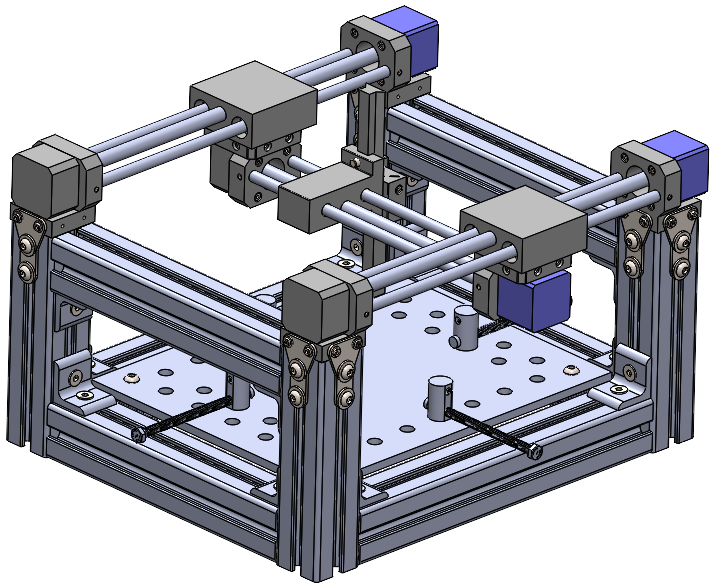
\includegraphics[width=.9\linewidth]{Sections/1 Indledning og Formalia/Media/Assembly.png}
\end{figure}
}

\begin{figure}[b]
    \centering
    
\includegraphics[width=.1\linewidth]{Sections/1 Indledning og Formalia/Media/logo.png}
\end{figure}


\thispagestyle{empty}
\begin{footnotesize}
\begin{minipage}[t]{0.48\textwidth}
\vspace*{-25pt}		

\includegraphics[height=4.0cm]{Sections/1 Indledning og Formalia/Media/aau_logo_da.pdf}
\end{minipage}
\hfill
\begin{minipage}[t]{0.48\textwidth}
{\small 
\flushright{ 
\textbf{\institute
} \\ Aalborg Universitet \\
}
}
\end{minipage}
\end{footnotesize}

\vspace*{20pt}

\begin{footnotesize}
\begin{minipage}[t]{0.48\textwidth}
\textbf{Titel:} \\
\thetitle \\
 
\textbf{ECTS:} \\
{\ectspoint} ECTS \\

\textbf{Semester:} \\
2. semester \\
%\textbf{Semestertema:} \\[0.5pt]\bigskip\hspace{2ex}%

\textbf{Projektperiode:} \\
{\periodfrom} til {\periodto} \\

\textbf{Projektgruppe:} \\
\groupname \\

\textbf{Gruppemedlemmer:} \\
\foreach \i in \theauthor{
    \i \\
}

\textbf{Vejleder:} \\
\suporvisor \\

\textbf{Rapport sideantal: \pageref{chap:endOfRapport}} \\
\textbf{Antal sider: \thelastpage}

\end{minipage}
\end{footnotesize}
\hfill
\linespread{1.15}\selectfont{
\begin{minipage}[t]{0.550\textwidth}
\textbf{Abstract:} \\[5pt]
\fbox{\parbox{8cm}{\smallskipThis project explores the mechanical design of a robot intended for the automated application of speckle patterns used in Digital Image Correlation (DIC). DIC is a non-contact optical measurement technique used to determine strain by measuring deformation in a given material by comparing images of a specimen before and after loading and deformation. A key requirement for accurate DIC measurements is the application of high-quality speckle patterns' random dot distributions with specific contrast, density, and dot size criteria. Current manual methods for applying such patterns, including airbrushing, stamping and marker-based techniques, are time-consuming and prone to unwanted variability in dot placement and size. This project aims to improve pattern consistency and reduce manual workload by developing a robot capable of reliably applying speckle patterns in macroscale on 2D surfaces. The report presents a detailed analysis of speckle pattern requirements, existing application methods, and relevant robotic design considerations. Based on this, a mechanical concept is developed that prioritizes precision, repeatability and adaptability to various object sizes and materials. 

\smallskip}}
\end{minipage}}

\begin{table}[b]
    \centering
    \begin{tabular}{m{\linewidth}}
         \textit{Indholdet af denne rapport er frit tilgængeligt, men udgivelse (med reference) af dette må kun gøres efter aftale med forfatterne}
    \end{tabular}
\end{table}

\thispagestyle{empty}
\chapter*{Forord}
Denne rapport er udarbejdet som en del af 2. semesterprojektet, svarende til 10 ECTS points, på bacheloruddannelsen i Mekanik og Produktion ved Aalborg Universitet. Projektet er gennemført i perioden 3. februar til 23. maj 2025 af projektgruppen 4.020A og har haft fokus på udviklingen af en robot til automatisk påføring af speckle patterns til brug ved Digital Image Correlation (DIC). 

Projektarbejdet har givet gruppen mulighed for at anvende og videreudvikle kompetencer inden for blandt andet mekanisk design, konceptudvikling og kravspecifikation, samt indhente viden om DIC-teknologi og relevante robotprincipper. Gennem arbejdet har gruppen opnået en dybere forståelse, for hvordan automatisering kan bidrage til øget præcision og ensarthed i eksperimentelle materialetest. 

Tak til vejleder, Niklas Kristian Kronborg Stagsted, for faglig sparring og konstruktiv feedback gennem hele projektforløbet. 

% Indsæt ai dekleration

\textbf{Large Language Models} er i denne rapport brugt til kodning af \LaTeX \, samt som sparringspartner under idegenerering.




\addcontentsline{toc}{chapter}{Forord}
\thispagestyle{Unifront}
\newpage
\chapter*{Symbolliste}

% der må ikke skrives i det her dokument, det skal gøres i "ordlisten"!!!


\begingroup
\setlength{\tabcolsep}{10pt} % Default value: 6pt
\renewcommand{\arraystretch}{1.5} % Default value: 1
\begin{table}[H]
    \centering
    \begin{tabular}{c c c}
         \textbf{Symbol} & \textbf{Betydning} & \textbf{Enhed} \\
         \hline
         \symbollist
    \end{tabular}
    \label{tab:symbolliste}
\end{table}
\endgroup

\chapter*{Forkortelser}

\renewcommand{\arraystretch}{1.5} % Default value: 1
\begin{longtable}{c c c}
\textbf{Forkortelse}  & \textbf{Forklaring} \\
\hline
\endhead
    DIC & Digital image correlation  \\
    DOF & Degrees of freedom\\
    FOV & Field of view \\
    HoQ & House of Quality \\
    IK & Inverse kinematic\\
    NEMA & National Electrical Manufacturers Association \\
    OR & Optimerings retning \\
    RV & Relative vigtighed \\
    2D & Todimensionel\\
    3D & Tredimensionel\\
   % 6082-T6 & Aluminiums legering DS-EN 573-3 \\
   % 6063-T5 & Aluminiums legering DS-EN 573-3 \\
   % 6560-T6 & Aluminiums legering ASTM B221-2 \\
\label{tab:forkortelser}
\end{longtable}

\thispagestyle{Unifront}
\newpage
\thispagestyle{Unifront}

\tableofcontents*

\thispagestyle{empty}
\newpage

\mainmatter
\pagestyle{Uni}
\setcounter{page}{1}

% ------  Kaptiler i rapporten -------
\newpage
\chapter{Indledning}
Digital Image Correlation (DIC) er en optisk målemetode, der anvendes til at vurdere spændinger i forhold til deformationer i materialer ved at analysere ændringer i digitale billeder af emner, før og efter belastning. DIC gør det muligt, at få målinger over større områder, hvor deformationer kan observeres og kvantificeres. Dette gør at DIC er en god metode til at undersøge komplicerede emner, i forhold til andre måleværktøjer som strain gauges og extensometre.

Et centralt element i DIC er brugen af speckle patterns, tilfældigt fordelte prikker, som påføres overfladen af testemnet. Den nuværende, manuelle påføring af speckle patterns, herunder airbrush, spraymaling eller tusch, er ofte tidskrævende og kan resultere i mønstre der ikke er optimale. Dette påvirker både målenøjagtigheden og genskabeligheden af DIC-analyser. Automatisering kan skabe et mere optimalt speckle pattern, samt åbne muligheden for genskabelige speckle patterns og dermed forbedre nøjagtigheden og pålideligheden af metoden.

Dette projekt fokuserer på mekaniske aspekter ved design af en robot til påføring af speckle patterns i makroskala på et 2D-plan. Gennem analysen af krav til DIC-metoden og speckle patterns, samt vurdering af eksisterende løsninger, udarbejdes et produkt, der har til formål at øge kvaliteten af DIC-metoden, samt reducerer arbejdsbyrden.




\plainbreak{2}
\section{Initierende problemstilling}
Projektet udarbejdes på baggrund af den følgende initierende problemstilling: \plainbreak{-0.1}
\begin{displayquote}  \centering 
\textit{Hvordan automatiseres påføringen af speckle patterns egnet til Digital Image Correlation ved brug af en robot.} %(til undersøgelse af materiale egenskaber).
\end{displayquote}


\begin{comment}
    Det kan evt, bruges i indledningen, at det har en præcision på 93%
    
    "The  suggested  measurement  method  has an  average  accuracy  of  more  than  93%  in estimating specimen displacements." https://www.researchgate.net/publication/374375688_Application_of_Digital_Image_Correlation_Method_in_Materials_-_Testing_And_Measurements_A_Review

    Digital Image Correlation (DIC) er en optisk målemetode, der anvendes til analyse af deformationer og spændinger i materialer, ved sammenligning af billeder fra en prøve før og efter belastning. Metoden er kendt for sin høje nøjagtighed, med en gennemsnitlig præcision på mere end 93\%, sammenlignet med strain gauge, og linear variable differential transformer (LVDT) \parencite{Zaya2023ApplicationReview}. 

Et godt speckle pattern opfylder en række af kriterier: det skal have en passende kontrast mellem de lyse og mørke områder i mønsteret, en tilfældig fordeling af prikker uden gentagelser samt en passende prikstørrelse i forhold til kameraets opløsning og overfladen på det testet materiale. Normalt påføres speckle patterns manuelt ved hjælp af en airbrush, spraymaling eller med en kuglepen, men denne manuelle proces kan føre til variationer i kvaliteten i mønsteret, hvilket kan påvirke både nøjagtigheden af målingerne og genskabeligheden af DIC-analysen.

For at imødekomme disse udfordringer kan automatisering med en robot være en løsning, der sikrer ensartede mønstre med præcist kontrollerede forhold. Dette kan forbedre nøjagtigheden af DIC-målinger og gøre processen mere effektiv og reproducerbar.

\textbf{\textit{Kommentare fra vejledermødet:\\}}
-Snakke om DIC og den kontekst det bruges i, og hvorfor det er vigtigt og hvorfor det er smart, at lave et helt projekt om en lille del af DIC. \\
-Gør det tydeligt, hvad motivationen for at lave en robot til speckle pattern er. 
-DIC er ikke kendt for høj nøjagtighed - 93\% er ikke højt. Det er brugt til at vurdere deformationer i hele objektet frem for observerbare dele. \\
-LVDT er formentlig et extensiometer. Der bruges primært strain gauges, LVDT og DIC. \\
- DIC er ikke præcis, men man kan få full field målinger, fremfor kun på enkelte punkter.  \\
- Forklar hvad et speckle pattern er i indledningen.  

\end{comment}

 

\chapter{Problemanalyse} \label{Problemanalyse}
Det følgende afsnit har til formål at afdække anvendelse og fremstilling af speckle patterns til brug ved DIC, herunder undersøgelse af hvilke parametre, der beskriver et optimalt speckle pattern. Derefter defineres og undersøges robotter for at opnå den nødvendige forståelse for deres mekanismer, så en løsning til fremstilling af speckle patterns kan udvikles.

% --- DIC ---
\section{Digital Image Correlation} \label{DIC afsnit}
DIC er en optisk metode, der anvender digitale billeder til at måle deformation, bevægelse og tøjning i materialer. DIC fungerer ved at sammenligne billeder taget før, under og efter deformation for at måle forskydninger og udregne tøjninger. Metoden gør det muligt at undersøge deformationer over hele emnet og omkring revner. (\cite{Zaya2023ApplicationReview})

\begin{figure}[H]
    \centering
    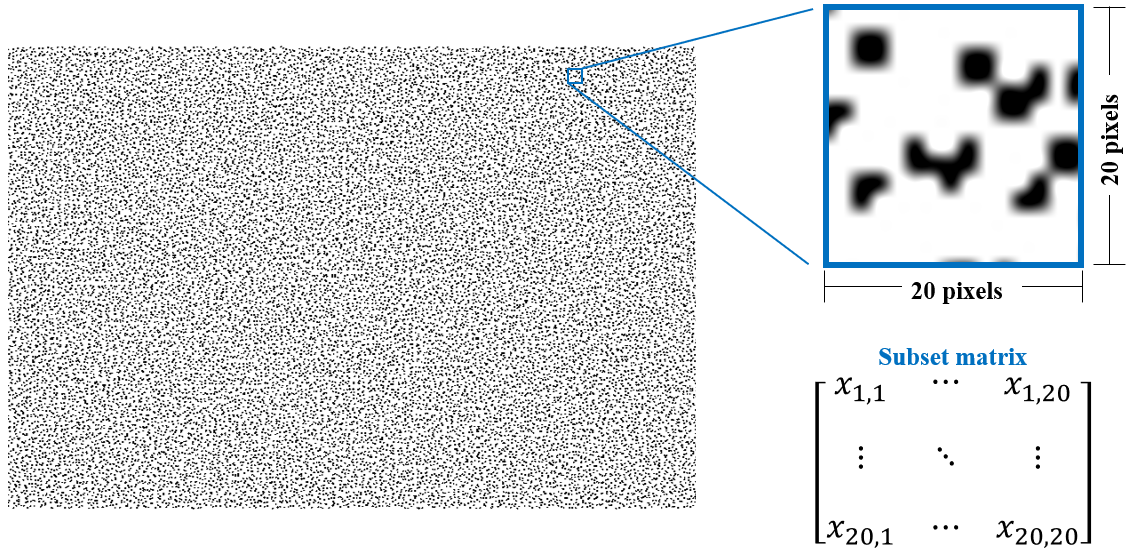
\includegraphics[width=0.85\linewidth]{Sections/2 Problemanalyse/Media/Speckle pattern subset matrix.png}
    \caption{Illustration af speckles pattern, i øverste højre hjørne ses et subset på $20 \times 20 \text{pixels}$ . Det er genereret med software fra Correlated Solutions (\cite{CorrelatedSolutions2025SpeckleInc.})}
    \label{fig:speckle pattern subset}
\end{figure} \plainbreak{-0.5}

DIC starter med et reference billede taget før deformation, eventuelt efterfulgt af billeder taget under deformationsprocessen, samt et billedet efter deformation. Computersoftware bruger forskellen mellem referencebilledet og de efterfølgende billeder, til at finde deformationer, som herefter udregnes til tøjninger i prøven. Softwaren gør dette ved at identificere subsets af pixels (se figur \ref{fig:speckle pattern subset}) i reference billedet, og derefter finder samme deformerede subset på billedet hvor emnet er deformeret. (\cite{Zaya2023ApplicationReview})

DIC benyttes både til undersøgelser af plane emner (2D), samt rumlige emner (3D). I 2D undersøgelser må materialet ikke deformere sig ud af planet, da denne bevægelse ikke kan blive set af kameraet. 3D DIC benytter sig af to eller flere kameraer, og er optimal i situationer, hvor et materiale bevæger sig fra planet til rummet (figur \ref{fig:2D og 3D DIC}).

\begin{figure}[H]
    \centering
    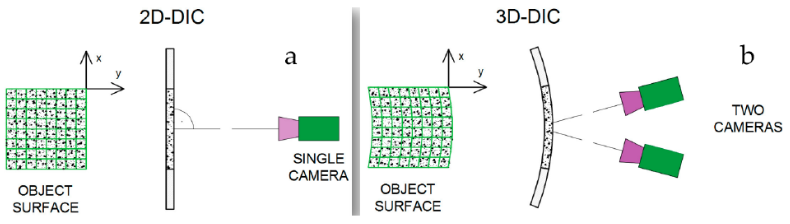
\includegraphics[width=0.9\linewidth]{Sections/2 Problemanalyse/Media/DIC 2D eller 3D.png}
    \caption{Opstilling af 2D og 3D digital image correlation (\cite{Wang2023FiberMonitoring})}
    \label{fig:2D og 3D DIC}
\end{figure} \plainbreak{-0.5}

Opstillingen med flere kameraer giver mulighed for, at tage flere billeder fra forskellige vinkler, og ved hjælp af stereo triangulering, danne en 3D model af objektet. (\cite{Byrne2020DigitalSoftware})


Speckle patterns opdeles i denne rapport i to dele, mikro- og makroskala. I denne rapport defineres mikroskala som den størrelse, der ikke kan opfanges med det blotte øje, og makroskala er den størrelse, der kan fanges med det blotte øje. Der vælges at arbejde i makroskala, med prikker ned til \SI{0,1}{mm} i diameter, fordi det vurderes, at være realistisk at lave speckle patterns i en størrelsesorden man kan se, og ikke mindre.


%Vinklen mellem to kameraer og objektet kaldes stereo vinklen. Denne vinkel kan justeres afhængig af ønsket resultat. Hvis man ønsker større undersøgelse rettet mod et plan, kan vinklen mindskes, og til en rumlig undersøgelse med bevægelse ud af planet, kan vinklen øges. Den optimale vinkel for 3D DIC er mellem 15\degree og 35\degree. (\cite{Bigger2018ACorrelation}) 



\subsection{Alternative målemetoder}
Alternativerne til DIC er primært strain gauges og ekstensometre. Generelt kan de betegnes som spotmålere, det vil sige de måler over et begrænset område, tilgengæld giver de mere nøjagtige målinger end DIC.

\begin{figure}[H]
    \centering
    \begin{subfigure}{0.48\textwidth}
        \centering
        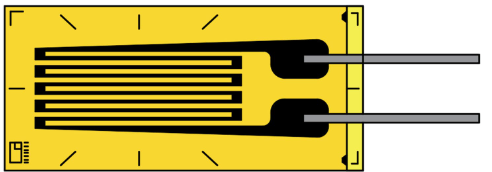
\includegraphics[width=0.8\linewidth]{Sections/2 Problemanalyse/Media/strain gauge.png}
        \caption{Lineær strain gauge der ikke er monteret \parencite{IndustrialQuickSearch2025PrinciplesGauges}}
        \label{fig:straingauge}
    \end{subfigure}
    \begin{subfigure}{0.48\textwidth}
        \centering
        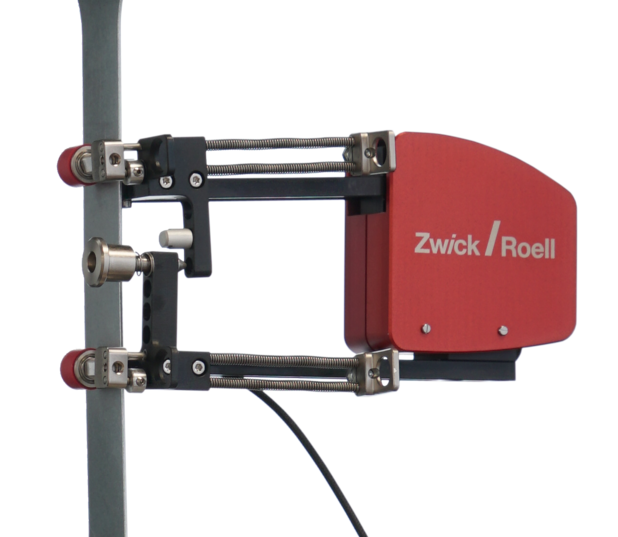
\includegraphics[width=0.7\linewidth]{Sections/2 Problemanalyse/Media/ekstensometer.png}
        \caption{Clip-On ekstensometer monteret \parencite{ZwickRoellExtensometers}}
        \label{fig:ekstensometer}
    \end{subfigure}
    \caption{}
    \label{alternativertildic}
\end{figure} \plainbreak{-0.5}

\textbf{Strain gauges} består af en tynd metalstribe, typisk i zigzaggede parallelle linjer (se figur \ref{fig:straingauge}), på et fleksibelt, isolerende materiale med en form for klistrende underside. Tøjningen findes ved måling af ændringen i modstand, jo mere den deformeres jo højere vil modstanden blive. 

\textbf{Ekstensometre} måler ændringen i afstanden mellem dens to arme, se figur \ref{fig:ekstensometer}. Ekstensiometre kommer i flere varianter der afhænger af,  hvordan armene påsættes emnet.


 

%Siden sin begyndelse i slut 1900-tallet, har DIC gennem årene udviklet sig, og blevet benyttet til en række af forskellige materialeundersøgelser og er blevet til en populær eksperimentel metode blandt andet grundet kosteffektivitet. Materialeundersøgelser som DIC har været igennem inkluderer metaller, polymerer, kompositter, samt biologiske materialer. Disse undersøgelser finder sted på både mikro- og makroskopisk skala, fra millimeter til flere meter. Herved har man også fundet materialer, som ikke er egnet til DIC grundet specifikke faktorer. Nogle af disse inkluderer: Gennemsigtige, bløde eller reflekterende materialer. Løsninger på disse lyder på overfladebelægning af gennemsigtig materiale, benytte speckles af matsort på reflekterende overflader. På bløde materialer er det mere besværligt, men et kamera med en høj rate af billeder i sekundet skal anvendes, grundet skrøbelighed og hurtig deformation. (\cite{Dong2017ACorrelation}; \cite{Bigger2018ACorrelation}) 


% --- Speckle patterns --- 
\plainbreak{2} \section{Speckle pattern} \label{Speckle pattern} 
Speckle patterns er betegnelsen for et billede eller område med prikker, der anvendes til måling af deformationer og tøjninger i materialer ved brug af DIC \parencite{Dong2017ACorrelation}. Prikkerne i et speckle pattern er ikke foruddefineret til at have én bestemt størrelse, form, kontrast, densitet og fordeling. Disse parametre afhænger af størrelsen på emnet der undersøges, kameraets opløsning samt påføringsmetoden. Eksempler på forskellige speckle patterns kan ses i figur \ref{fig:speckle pattern}.\\

\begin{figure}[H]
    \centering
    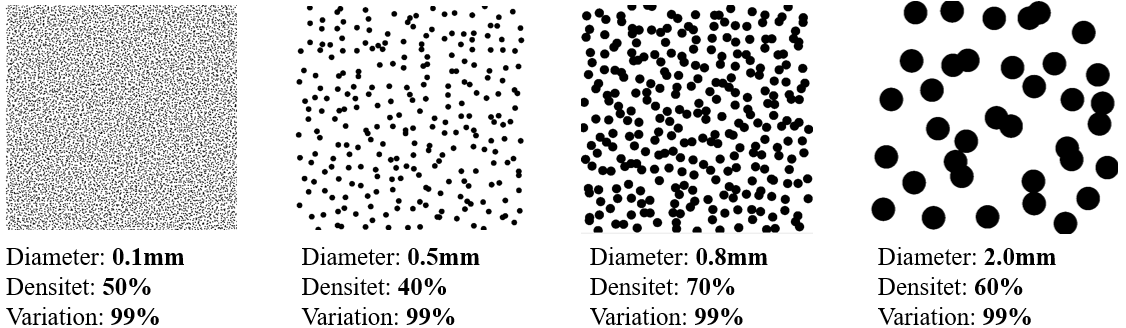
\includegraphics[width=\linewidth]{Sections/2 Problemanalyse/Media/speckle pattern forskellige.png}
    \caption{Eksempler på computergenereret speckle patterns med forskellig densitet og prikstørrelse. Speckle pattern er genereret med software fra Correlated Solutions (\cite{CorrelatedSolutions2025SpeckleInc.})}
    \label{fig:speckle pattern}
\end{figure} \plainbreak{-0.5}

Præcisionen af DIC afhænger blandt andet af det anvendte speckle patterns kvalitet, der kan vurderes ved brug af softwareprogrammer. Programmerne benytter forskellige metoder til kvalitetsvurdering, der vurderer parametre som størrelse, form og fordeling af prikkerne.  
\plainbreak{1} \subsection{Optimale speckle patterns} \label{Optimale speckle patterns}

Et godt speckle pattern er karakteriseret ved høj kontrast mellem prikker og baggrund, og et tilfældigt mønster, der er jævnt fordelt og udgør mellem 50\% og 70\% af billedet. Prikkerne skal have en ensartet radius, samt have en størrelse på mellem $3\times3$ og $5\times5$ pixels. Derudover skal prikkerne være indenfor kameraets field of view (FOV). I denne rapport referer FOV til længden af det område kameraet observerer, det er dermed en konsekvens af dets brændvidde og afstand til emnet. (\cite{Dong2017ACorrelation}; \cite{Su2022Glare:Pattern}; \cite{Gagnon2024ThePatterns}).  


%------
\subsubsection{Høj kontrast}\plainbreak{-0.4} 
DIC benytter gray-level til vurdering af prikkernes placering på overfladen. Gray-level er en grå-skala værdi fra 0\% til 100\%, der beskriver lysintensiteten i et enkelt pixel. Et gray-level på 100\% ses som hvid, hvor 0\% er helt sort, gray-level værdien angiver mængden af lys. Værdierne angives fra 0 til 255 for et 8-bit kamera. Det er nødvendigt med høj kontrast, så kameraet kan opfange forskellen mellem prikker og baggrund. Ofte bruges sorte prikker på hvid baggrund, eller hvide prikker på sort baggrund, idet disse har størst forskel mellem prikkerne og baggrundens gray-level. Forskellen mellem baggrund og prikker skal være på minimum 52 point, for at opnå en optimal værdi, skal denne forskel ligge på 130 point og derover (\cite{Reu2015AllContrast}; \cite{Bigger2018ACorrelation}).


%----- 
\newpage
\subsubsection{Størrelse på prikkerne} \plainbreak{-0.4}
Prikkernes størrelse har betydning for, hvordan prikkerne opfanges af kameraet, samt softwaren bearbejder dataen. For at opnå et optimalt resultat skal prikkerne være større end tre pixels, hvilket afhænger af kameraets opløsning og FOV. Den minimale diameter på prikkerne ($\diameter_{min}$), er derfor afhængig af FOV og antallet af pixels ($n_{pixels}$), som det fremgår af formel \ref{equ:prikstørrelse-Ø_min}. FOV definerer enten bredden eller højden på området, indenfor kameraets synsfelt, der er påført speckle pattern og måles i millimeter. Formlen bruges til at give et estimat, af den minimale diameter prikkerne må have, for at give et optimalt resultat ved DIC. $\diameter_{min}$ beregnes separat for henholdsvis bredden og højden af FOV. Hvis $\diameter_{min}$(bredden) $\neq \diameter_{min}$(højden), benyttes den største diameter (\cite{Reu2014AllAliasing}).
 \begin{equation} \label{equ:prikstørrelse-Ø_min}
     \diameter_{min} = \frac{FOV}{n_{pixels}} \cdot n_{min \ \vee \  max \ pixels} 
 \end{equation}
Prikker mindre end $3\times3$ pixels er vanskelige at bestemme centrum af, idet en prik på $1\times1$ pixels der ligger mellem to pixels vil give en slørret afbildning i gray-level, hvorved kontrasten mellem prik og baggrund mindskes, hvilket medfører en stigning i systematiske fejl. Yderligere øges præcisionen ved brug af prikker over $3\times3$ pixels, fordi det bliver tydeligere på gray-level, hvor prikken er lokaliseret, da den vil dække flere pixels, selvom prikken er placeret mellem to pixels, som det er illusreret på figur \ref{fig:gray-level}. (\cite{Reu2014AllAliasing}; \cite{Cui2024EffectError})

\begin{figure}[H]
    \centering
    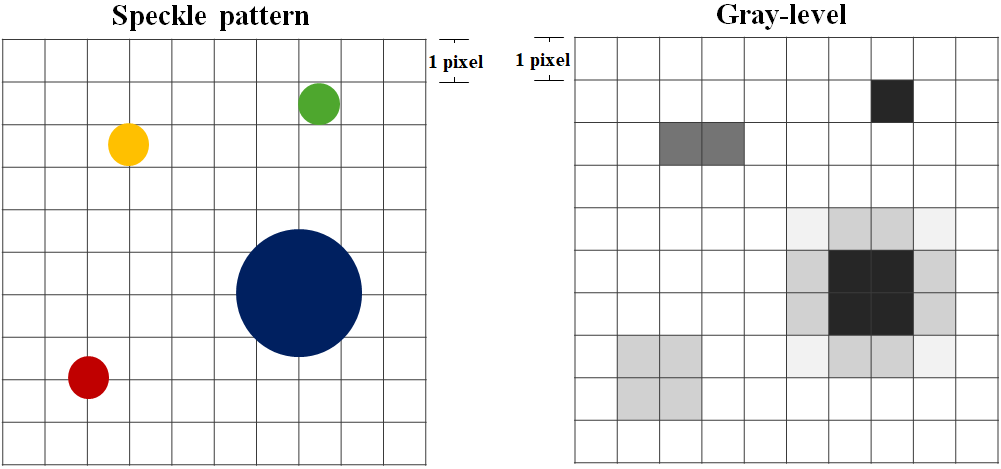
\includegraphics[width=0.8\linewidth]{Sections/2 Problemanalyse/Media/gray-level.png}
    \caption{Illustration af computersoftwares opfattelse af sepckel patterns. Gitteret illustreret et subset på $10\times10$ pixels. Den \textcolor{red}{røde}, \textcolor{greenB}{grønne} og \textcolor{gulny}{gule} prik er alle $1\times1$ pixels, placeret forskelligt i gitteret. Den \textcolor{blue}{blå} prik er $3\times3$ pixels.}
    \label{fig:gray-level}
\end{figure} \plainbreak{-.5}

Prikkerne kan ikke være uendeligt store, da de er begrænset af FOV, kameraets opløsning, det procentvise forhold prikkerne må dække af hele overfladen, samt størrelsen på overfladen der undersøges. Når prikker er større bliver softwaren nød til at gøre brug af tilsvarende større subsets for at garantere unikke subsets. Der skal altså findes et kompromis mellem størrelsen af subsets, dermed nøjagtighed, og systematiske fejl fra prikker placeret på kanten af pixels. Dette kompromis er en prikstørrelse på mellem $5 \times 5$ og $8 \times 8$ pixels. (\cite{Haddadi2008UseTechnique}; \cite{Crammond2013SpeckleCorrelation}; \cite{Dong2017ACorrelation};  \cite{Gagnon2024ThePatterns})


Ved forventning om store deformationer, hvor mindre deformationer er uvæsentlige at undersøge, kan større prikker bruges, uden det har betydning for det der ønskes undersøgt. Overfladens størrelse medvirker til den maksimale størrelse prikkerne kan have, idet store overflader, kan benytte prikker af en større størrelse til subsets, fordi FOV er større (se \ref{equ:prikstørrelse-Ø_min}). Prikkerne i det samme speckle pattern kan variere mellem tre pixels og otte pixels, men for optimal måling skal størrelsesforskellen på prikkerne i det samme speckle pattern holdes minimal(\cite{Crammond2013SpeckleCorrelation}; \cite{Gagnon2024ThePatterns}).  

%-----
\subsubsection{Tilfældigt og isotropt}\plainbreak{-0.4}
Identifikationen af et subset's bevægelse efter deformation af emnet, er kun mulig, hvis prikkerne er arrangeret i et mønster der ikke gentages. Hvis de ligger på linje er det ikke muligt at se hvis prikkerne er forskudt langs den linje (\cite{Zaya2023ApplicationReview}).

%----
\subsubsection{Fordeling af prikkerne}\plainbreak{-0.4}
Et godt speckle pattern har en 50\% til 70\% dækning af prikker. Prikkerne skal være jævnt fordelt med minimum tre pixels mellem alle prikkerne. Hvis prikkerne er for tætte på hinanden, kan softwaren have det vanskeligt med at identificere, om det er én stor prik eller flere små prikker, hvilket øger usikkerheden ved måling. (\cite{Reu2015AllDensity}; \cite{Caliskan2024InvestigationDIC})

\begin{figure}[H]
  \centering
    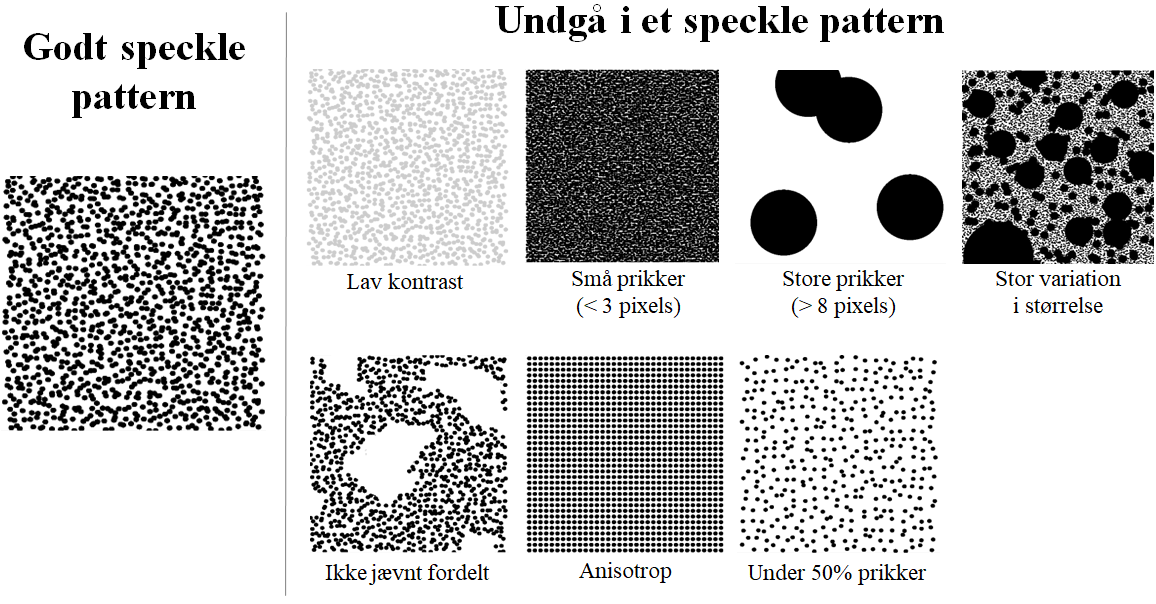
\includegraphics[width=0.9\textwidth]{Sections/2 Problemanalyse/Media/speckle pattern.png}
    \caption{Illustration af fejlkilder ved produktion af speckle pattern til DIC. Speckle pattern er genereret med software fra Correlated Solutions (\cite{CorrelatedSolutions2025SpeckleInc.})}
    \label{fig:godt speckle pattern}
\end{figure} \plainbreak{-0.4}

Figur \ref{fig:godt speckle pattern} illustrerer fejlkilder i speckle patterns, der mindsker præcisionen af DIC. Kriterierne for et godt speckle pattern er gældende for både 2D og 3D.


%-----
\subsubsection{Forblive på overfladen} \plainbreak{-0.4}
Det er nødvendigt, at prikkerne forbliver på og deformerer med overfladen af emnet der undersøges. Resultaterne af DIC er ikke retvisende, hvis prikkerne flytter sig uafhængigt af det undersøgte emne. Det er nødvendigt, at prikkerne flytter sig med emnet og ikke påvirker dets egenskaber. Derudover skal prikkerne ikke have tydelig ændring i gray-level eller geometri efter deformation.
(\cite{Dong2017ACorrelation} ; \cite{Zaya2023ApplicationReview}). \label{par:overfladen}



% --- Fremstilling ---
\plainbreak{2} \section{Fremstilling af speckle pattern} \label{Fremstilling af Speckle pattern}
Påføring af et speckle pattern i makroskala på en 2D flade, gøres på nuværende tidspunkt primært med enten spraydåse eller stempler. Det kan også gøres ved andre metoder såsom tusch eller midlertidige tatoveringer \parencite{Dong2017ACorrelation, Quino2021SpeckleEndurance}. Tidligere beskrevet i afsnit \ref{DIC afsnit}, afgrænses projektet til at skulle fremstille prikker i makroskala på $\geq \SI{0,1}{mm}$. Ved fremstilling af speckle pattern til DIC, ønskes det at parametrene er optimale, som beskrevet i afsnit \ref{Optimale speckle patterns}. 


\subsubsection{Spraydåser og Airbrush} \plainbreak{-.4}
Spraydåser og airbrushes producerer speckle patterns ved brug af trykluft til at blæse maling ud på en overflade. Spraymetoder er gode til at dække et område hurtigt og forholdsvist tilfældigt, idet malingens position kun kan bestemmes ved at ændre afstand til emnet, og retning som malingen udsendes i. Dette betyder, at malingen kan samles i større klumper, eller blive for sig selv i små pletter, der skaber unikke mønstrer, med stor variation i prikstørrelser. Dette kan være en udfordring, fordi der kan skabes for store mørke områder, eller kan ændre overfladetykkelsen. Derudover er airbrush og spraydåser begrænsede i, hvor store prikmønstrer de kan skabe. Dette overkommes ved at modificere på afstanden mellem emnet og dysen, dysens diameter, tryk i dysen og tykkelsen af væsken.\parencite{Dong2017ACorrelation, Quino2021SpeckleEndurance} 

Spraydåsen og airbrushen er ikke ens, og der er fordele ved, at bruge airbrush frem for spraydåser. Forskellen mellem airbrush og spraydåse kan ses på figur \ref{Spraymetode}, hvor de to billeder til venstre (a,b) er lavet med airbrush, og de to til højre (c,d) er udført med spraydåse. Her giver airbrushen et mere udspredt speckle pattern, og en større variation i prikstørrelse, som øger muligheden for unikke mønstre. Spraydåsen giver dog større risiko for afvigelse i prikstørrelserne, så der altid vil være prikker, der enten er for store eller for små til det ønskede speckle pattern. \parencite{Crammond2013SpeckleCorrelation}

\begin{figure}[H]
    \centering
    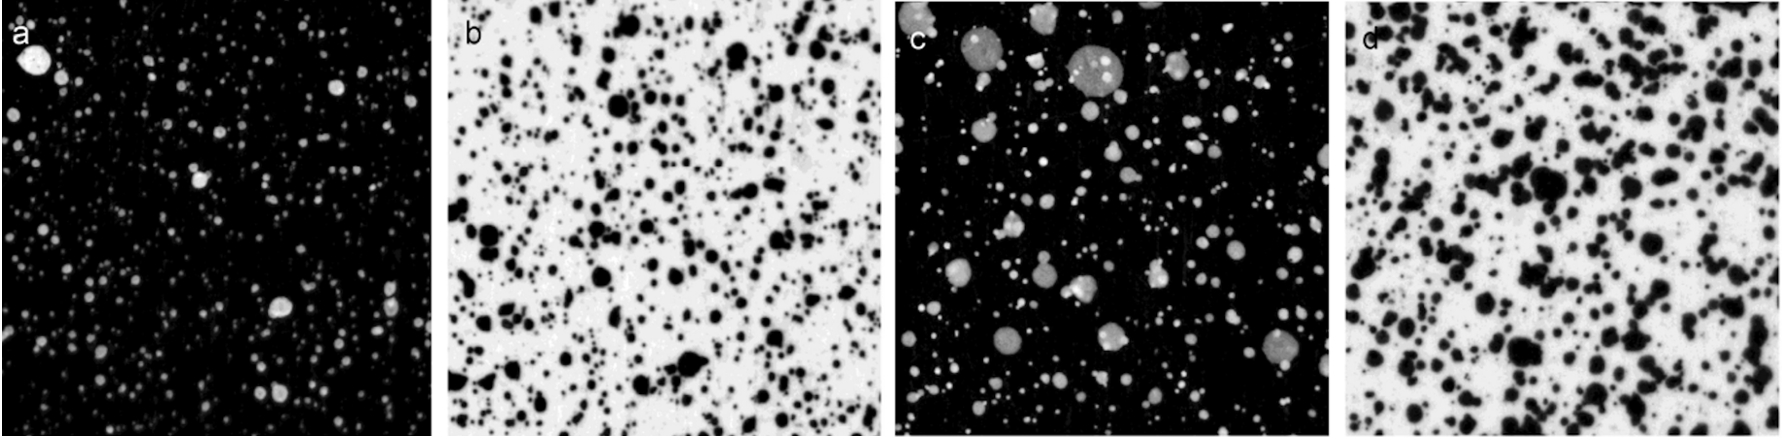
\includegraphics[width=1.0\linewidth]{Sections/2 Problemanalyse/Media/AirvsSprayinline.png}
    \caption{Speckle patterns med Airbrush og spraydåse. Her er a og b med Airbrush og c og d med Spraydåse \parencite{Crammond2013SpeckleCorrelation}}
    \label{Spraymetode}
\end{figure} \plainbreak{-0.5}


Spraydåsen er en priseffektiv metode til at påføre et  speckle pattern, hvor en spraydåse med 400 mL maling kan købes for 39,95kr. i Harald Nyborg (17.3.2025) \parencite{HaraldNyborg2025ColorWorksMat}. En airbrush har flere specialdele og kræver en kompressor for at virke, med det resultat, at den koster mere og anskaffe, modsat spraydåser \parencite{Dong2017ACorrelation}. Et airbrushsæt kan købes fra Amazon til omkring 600kr \parencite{TIMBERTECH2025Amazon.comAirbrush}.



\subsubsection{Stempel og stempelrulle} \plainbreak{-0.4}
Stemplet og stempelrullen er simple værktøjer til fremstilling af speckle pattern, da de ikke kræver andet end blæk at benytte. Anskaffelsesprisen er højere for stempelruller end airbrushes og spraydåser, hvor et sæt med 6 stempler, 6 ruller og noget blæk koster 2350\$ ($\simeq$ 16700 DKK, d. (25.2.2025)) hos Correlated Solutions. Eksempel på en stempelrulle kan ses i figur \ref{fig: Stempelrulle}. De størrelser der kommer i sættet fra Correlated Solutions, har stempelruller med prikdiametre fra $\SI{0,18}{mm}$ til $\SI{5,08}{mm}$, hvilket ved 1920:1080 opløsning, vil give en FOV fra $\SI{4,3}{cm}$ til $\SI{325}{cm}$. \parencite{CorrelatedSolutions2025VICCorrelation}

Stempler og rullerne virker ved, at blæk påføres deres overflade, som efterfølgende rulles over overfladen på emnet, hvor blækket overføres og efterlader et speckle pattern. Hvert stempel skaber mønstrer i en bestemt størrelse, hvilket begrænser antallet af forskellige emner og FOV'er det enkelt stempel kan bruges på, for at ramme 5-8 pixels pr. prik, som defineret i afsnit \ref{Speckle pattern}. \parencite{Dong2017ACorrelation}



\begin{figure}[H]
    \centering
    \begin{subfigure}{0.46\textwidth}
        \centering
        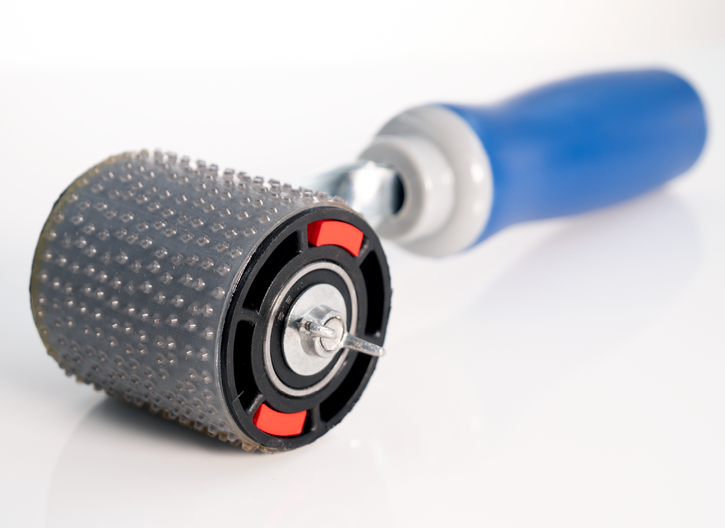
\includegraphics[width=.98\linewidth]{Sections/2 Problemanalyse/Media/Roller.png}
        \caption{Stempelrulle (\cite{CorrelatedSolutions2025VICCorrelation})}
        \label{fig: Stempelrulle}
    \end{subfigure}
    \begin{subfigure}{0.49\textwidth}
        \centering
         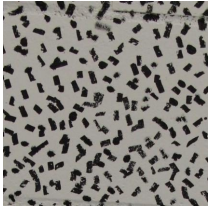
\includegraphics[width=0.7\linewidth]{Sections/2 Problemanalyse/Media/Tusch.png}
         \caption{Speckle pattern med overstregningstusch og lav densitet \parencite{HoseinSalmanpour2013PDFWalls}}
        \label{SpeckleTusch}
    \end{subfigure}
    \caption{}
    \label{fig:rulle og tush}
\end{figure} \plainbreak{-0.5}


\subsubsection{Tusch og andre skriveredskaber}  \plainbreak{-0.4}
En anden metode til påføring af speckle pattern, er tuscher og andre skriveredskaber, der sikre at prikkerne forbliver på overfladen af emnet under deformation. Et sæt med fire tuscher med en diameter på mellem \(\SI{0,1}{mm}\) og \(\SI{0,7}{mm}\) koster 13\$ ($\simeq$ 90 DKK, d. (6.3.2025)) \parencite{STAEDTLER2025Amazon.comTousch}. Metoden kræver, at prikkerne sættes manuelt én efter én på overfladen. Denne metode er tidskrævende, og kan være vanskeligt at opnå optimale parametre med, hvilket kan medføre fejlmålinger ved DIC, grundet mangel på nøjagtighed, som beskrevet i afsnit \ref{Speckle pattern}. Fordelen ved at prikkerne placeres manuelt er, at mønsteret ikke bliver isotropt. 
Det er et problem at prikkernes afstand mellem hinanden kan variere, da der kan skabes pletter, der er for store, eller områder med for lidt dækning af prikker, så der ikke kan observeres en deformation i de områder. Et eksempel på et speckle pattern tegnet med overstregningstusch kan ses i figur \ref{SpeckleTusch} \parencite{HoseinSalmanpour2013PDFWalls}. Usikkerheden ved metoden kan mindskes, hvis tiden der bruges på at sætte prikkerne øges. 





%Det er muligt at finde specielle tuscher eller kuglepenne, der er lavet med meget små spidser, så der kan laves prikker med en diameter på 100$\mu m$, som kan bruges i FOV'er helt ned til 2,2cm på langs (med en opløsning på 1920:1080).\parencite{Dong2017ACorrelation}.  her kan det blive et problem, da usikkerhederne kan medføre at der kommer klatter af ren farve eller andre fejl såsom mere farve end 70\% eller mindre end 50\%, som kan medføre fejlmålinger i DIC, grundet mangel på præcision (\ref{Speckle pattern}). Dette er muligt at undgå, hvis der bruges endnu længere tid på at gøre sine prikpositioner perfekte, som medfører mere tid brugt ved mindre skala.


\subsubsection{Midlertidig tatovering}  \plainbreak{-0.4}
En midlertidig tatovering, bruges til at overføre et bestemt mønster over på en flade. Dette fungerer ved, at der genereres et speckle pattern, som laserprintes ind på tatoveringspapiret. Herefter kan tatoveringen klistres på den ønskede overflade, hvorefter den vædes, så blækket overføres og forbliver på overfladen. Prisen på to A4 ark printbart papir til midlertidige tatoveringer koster 9.99\$ ($\simeq$ 69 DKK, d. 17.3.25) \parencite{SilhouetteAmerica2025TemporaryClearMEDIA-TATTOO-3T}. Det kræver en laserprinter, for at kunne printe en midlertidig tatovering, hvilket øger anskaffelsesprisen for denne metode.\parencite{Quino2021SpeckleEndurance}

\begin{comment}
    \begin{figure}[H]
    \centering
    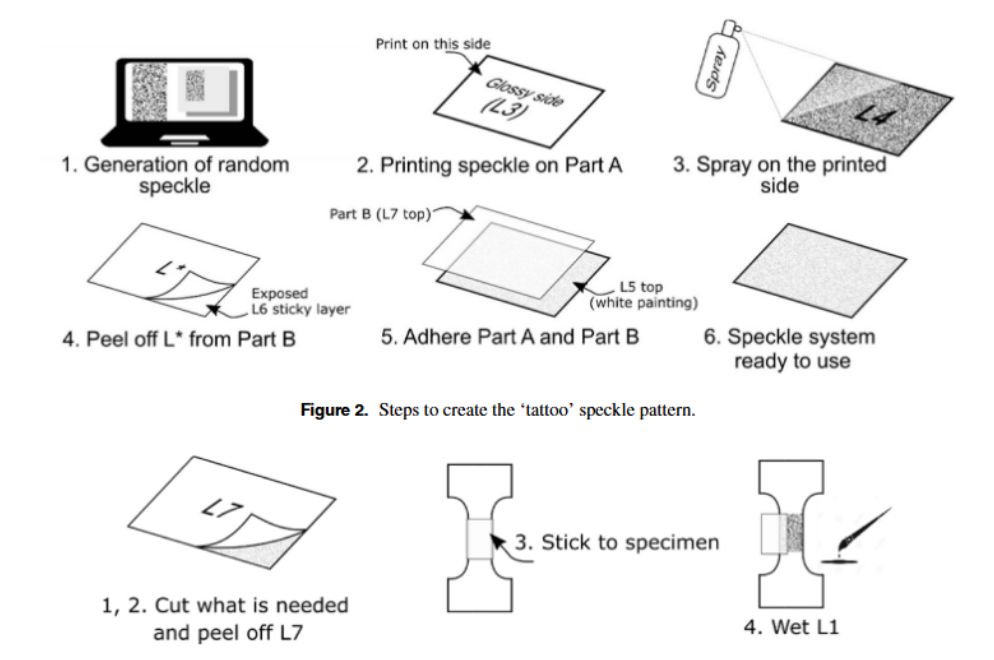
\includegraphics[width=0.8\linewidth]{Sections/2 Problemanalyse/Media/Temporary tattoo.png}
    \caption{Fremgangsmåde ved påføre af midlertidig tatovering med speckle pattern \parencite{Quino2021SpeckleEndurance}}
    \label{Midlertidigtatovering}
\end{figure}
\end{comment}



\subsection{Robotter til fremstilling af speckle pattern}  \label{Robotter til fremstilling af speckle pattern}
De nuværende produkter på markedet, der benyttes til fremstilling af speckle pattern, kræver manuelt arbejde og har varierende nøjagtighed i densitet og størrelse af prikker. På baggrund heraf vurderes det, at brugen af robotter til fremstilling af speckle patterns kan automatisere processen og har potentiale for at øge genskabeligheden. Sådan en løsning muliggør altå at der kan laves mere ensartetede prøver af flere af samme emnetype og dermed øges nøjagtigheden af DIC.


%Den mest brugte metode er spraydåsen, altså spraydåser og airbrush \parencite{Dong2017ACorrelation, Quino2021SpeckleEndurance}. Det vil altså være optimalt at kunne lave en løsning, der er mere effektiv end denne løsning. Spraymetoden er optimeret i forhold til pris og påføringshastighed, hvor spraydåser er engangsforbrug, og airbrush kan genbruges, men kræver en kompressor og maling. Det er derfor svært at slå disse to i pris og påføringshastighed, og det er derfor et ønske at lave et bedre produkt, som er bedre til at danne speckle patterns end spraymetoden er.

%En af de ting som spraymetoden ikke er god til, er at den er lidt for tilfældig, og store mængder maling kan samle sig på samme sted. Det vil derfor være et ønske, at løsningen skal kunne skabe et præcist mønster pålideligt, hvilket indebærer at der ikke skabes prikker mindre end 3 og større end 7 pixels (\ref{Speckle pattern}).

 

% --- Robotter --- 
\plainbreak{2} \section{Robotter} \label{Robotter}

Robotter er et mekanisk eller mekatronisk system, der selvstændigt eller delvist selvstændigt kan udføre én eller flere handlinger. Systemet styres typisk af en programmerbar styreenhed, der enten kan følge forudbestemte instruktioner eller tilpasse sin adfærd baseret på sensorinput. Robotter anvendes ofte til at automatisere opgaver, hvor der er krav om gentagelse, præcision eller effektivitet, og hvor manuel udførelse kan være forbundet med variation eller upræcise resultater. En robot består grundlæggende af flere integrerede systemer, der sammen muliggør kontrol over bevægelser og handlinger. Det mekaniske system danner grundstrukturen og kan være enten stationært eller bevægeligt, afhængigt af hvordan det skal interagere med emnet. \parencite{TextbookofRobotics}

%På baggrund af afsnit \ref{Fremstilling af Speckle pattern}, vurderes det, at robotter med fordel kan anvendes til fremstilling af speckle patterns. Manuelle metoder til at påføre speckle patterns, som for eksempel brug af airbrush eller tusch, kan føre til variationer i kvaliteten af mønstret. Disse variationer kan have en negativ indvirkning på nøjagtigheden og reproducerbarheden af målinger i DIC. Ved at anvende en robot forventes det, at påføringsprocessen kan standardiseres, hvilket sikrer en mere ensartet kvalitet og dermed mere pålidelige måleresultater.

%En vigtig del af robotten er påføringsmekanismen, som kan variere alt efter metode. Den kan for eksempel være baseret på sprøjteteknikker som airbrush, trykbaserede metoder som stempling eller andre teknologier, der overfører et prædefineret mønster, eksempelvis via print eller midlertidige tatoveringer. \parencite{TextbookofRobotics}

For at opnå nøjagtige bevægelser indgår der typisk sensorer i robotløsninger, der kontroller, at den teoretiske bevægelse også er udført i virkeligheden. Disse sensorer kan være kameraer, afstandsmålere eller kraftmålere, som giver systemet mulighed for at opdage afvigelser. Sensorerne sender data tilbage til styreenheden, som kan være en mikrocontroller eller computer, der i realtid kan behandle dataen og foretager de nødvendige justeringer. Dette samarbejde mellem sensorer, styreenhed og mekaniske komponenter er afgørende for, at kunne udføre de ønskede bevægelser og handlinger med nøjagtighed. \parencite{BasicsofRobotics}

Hvilken type robot, der kan være velegnet til opgaven, afhænger af en række forskellige faktorer. Eksempelvis kan størrelsen og geometrien på de testemner, der arbejdes med, have indflydelse på, hvordan systemet bør være udformet og bevæge sig i forhold til emnet. Desuden kan der være forskelle i, hvordan forskellige løsninger håndterer bevægelse, positionering og interaktion med omgivelserne. Derfor er det relevant at undersøge, hvilke forskellige typer af robotter der findes, og hvordan de adskiller sig fra hinanden.
\plainbreak{1}\subsection{Robottyper} \label{Robottyper}
Robotter kan klassificeres på forskellige måder afhængigt af den opgave de udfører, miljøet de gør det i, design og autonominiveau. Af de kategorier der er beskrevet i ISO 8373:2021 \parencite{ISO2021ISOVocabulary} og \cite{IFR2023World2023} er der to relevante kategorier for projektet. Desuden er printere og 3D FDM printere også inkluderet, da de udfører lignende opgaver.

\textbf{Industrirobotter} er automatiserede og programmerbare maskiner, der bruges i industrielle miljøer til opgaver såsom samling, svejsning og malerarbejde \parencite{IFR2023World2023}. Industrielle robotter kommer i alle størrelser, men kræver, til forskel fra de andre kategorier, særlig infrastruktur omkring dem. Det kan fx være indhegninger for robot arme, som vist på figur \ref{fig:irb7710pic}. De skal dermed ikke tage højde for mennesker, og bruges ofte til at udføre opgaver, hvor det er for dyrt eller farligt at ansætte folk \parencite{ABB2023IRBSeries, ISO2021ISOVocabulary}. 

\begin{figure}[H]
    \centering
    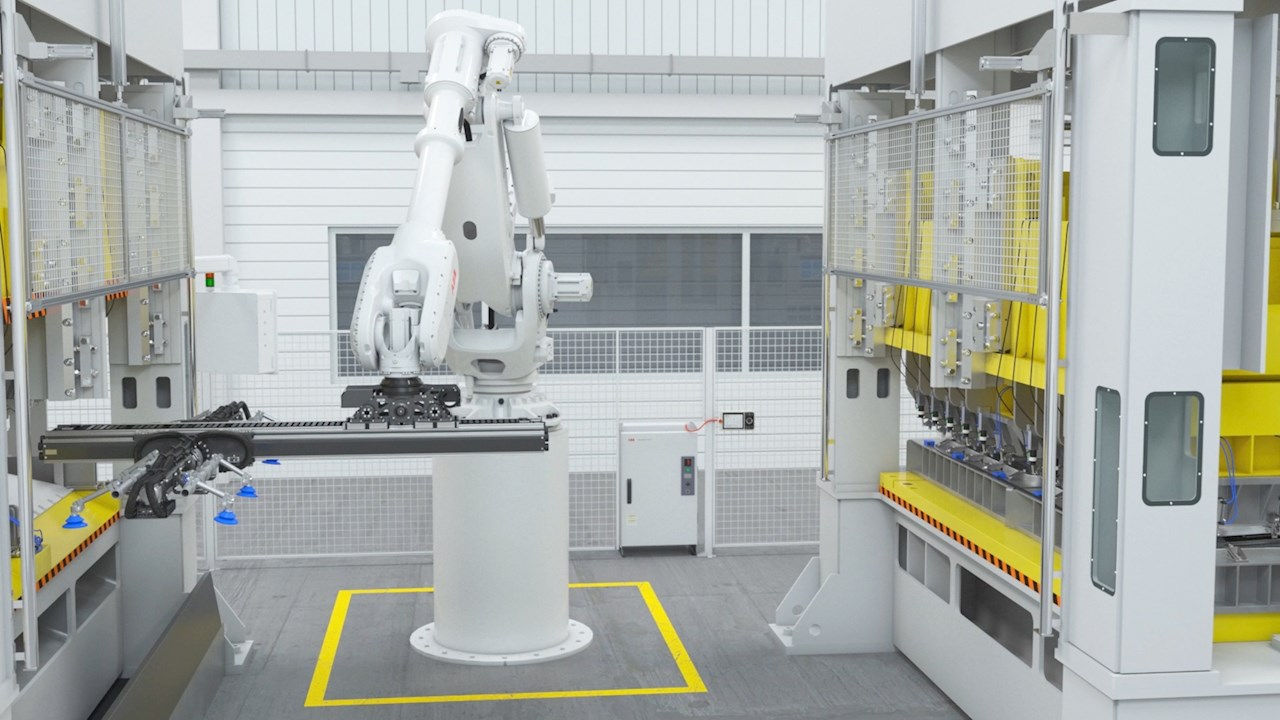
\includegraphics[width=0.6
    \textwidth]{Sections/2 Problemanalyse/Media/irb7710.jpg}
    \caption{IRB-7710 robotarm fra ABB \parencite{ABB2023IRBSeries}}
    \label{fig:irb7710pic}
\end{figure} \plainbreak{-0.5}
\textit{Eksempel:} ABB's IRB-robotter, serien indeholder mange forskellige størrelser af robotter. På figur \ref{fig:irb7710pic} ses model 7710, som er i den store ende og har en løftekapacitet på op til \SI{500}{kg}. På figuren er den sat op til at flytte store plader fra en stor maskine til en anden, robotten er praktisk her, da den kan løfte pladen fra midten af den ene maskine, og placere den i midten af den anden.
    
\textbf{Collaborative Robots (Cobots)} er designet til at arbejde sikkert sammen med mennesker i fælles arbejdsområder. De er ofte udstyret med sensorer og avancerede kontrolsystemer for at sikre at de kan koeksistere sikkert med mennesker \parencite{IFR2023World2023}. Her er sikkerhed altså en meget høj prioritet. Til forskel fra Servicerobotter er denne type ofte mere generaliserede og designet til at kunne arbejde sammen med mennesker, ikke blot i samme miljø.

\begin{figure}[H]
    \centering
    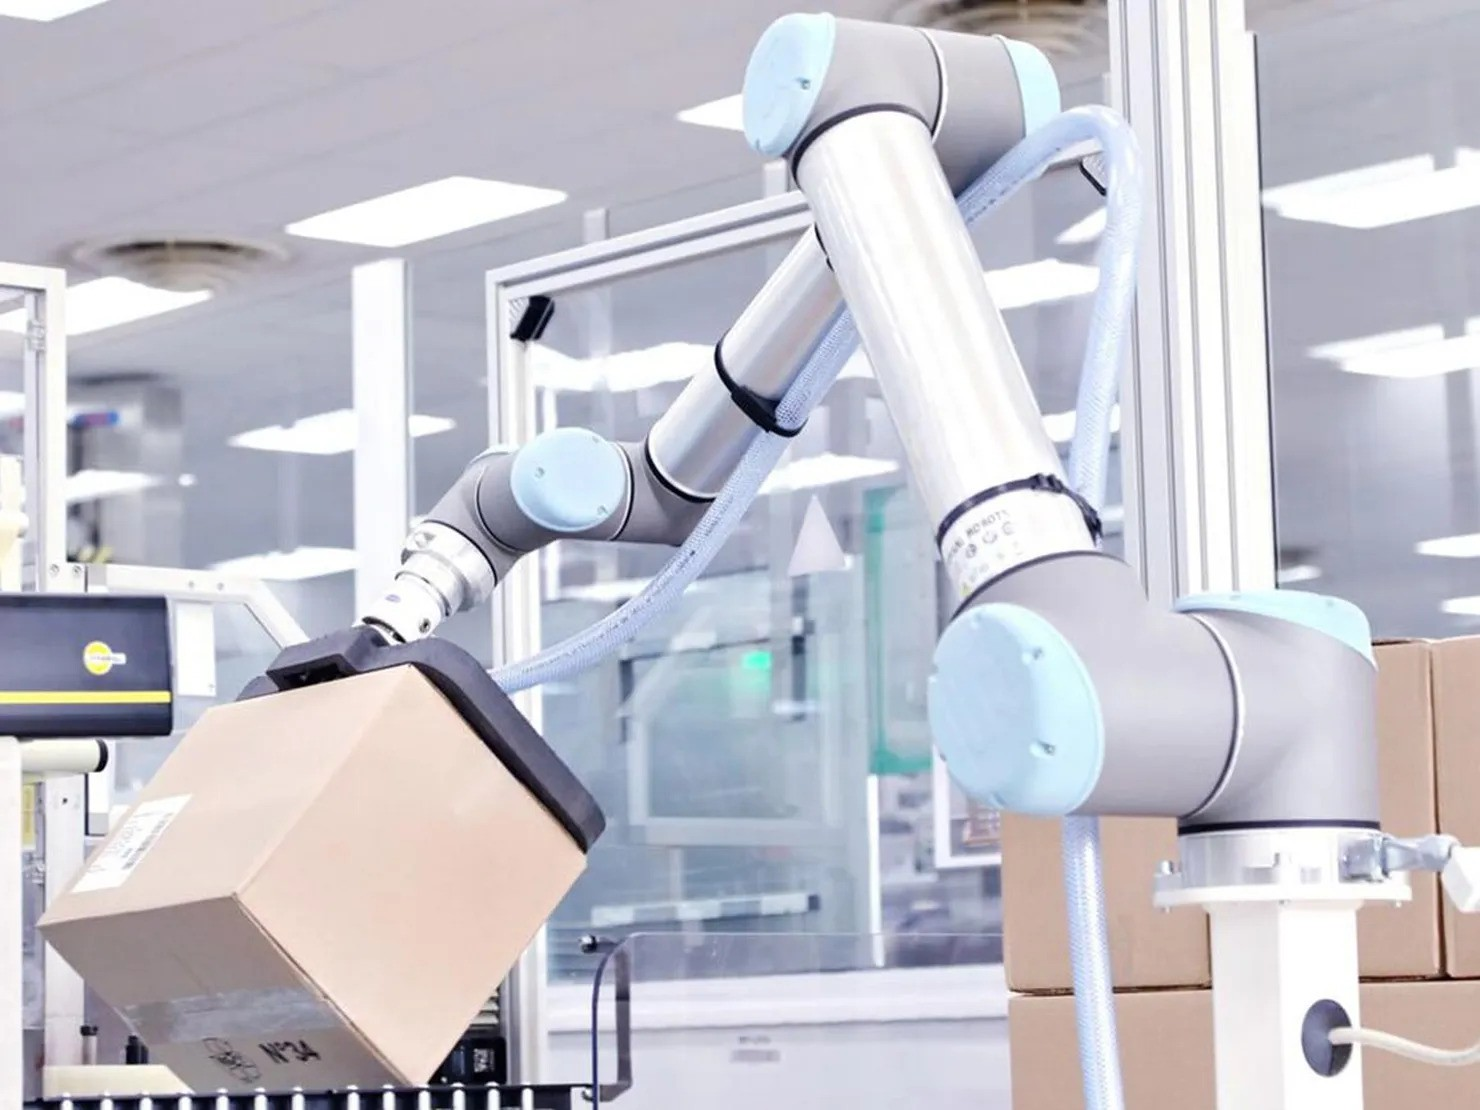
\includegraphics[width=0.5\linewidth]{Sections/2 Problemanalyse/Media/URrobot.jpg}
    \caption{UR5, et letvægt Cobot lavet i Danmark \parencite{2023URSeries}}
    \label{fig:ur5pic}
\end{figure} \plainbreak{-0.5}

\textit{Eksempel:} Universal Robots' UR-serie \parencite{2023URSeries}. Designet til at være flexible, billig og let. Primært tænkt til at samle op, flytte og placere. Fx kan den placere en del foran et mennesker, der kan udføre noget arbejde, hvorefter UR5 kan flytte den væk igen. Cobots bruges altså til at automatisere simple handlinger hvorimod mennesker stadig udføre mere kompliceret arbejde.

\textbf{Printere} er en type maskine, hvor et printhoved bevæger sig hen over en overflade for at afsætte små dråber væske i et præcist mønster. Systemet består typisk af en mekanisk struktur, der styrer printhovedets bevægelser i én retning, mens underlaget enten er stationært eller bevæges i en vinkelret retning. Bevægelsen kontrolleres af motorer, som sikrer en jævn og præcis føring, hvilket gør det muligt at opnå en ensartet fordeling af materialet på overfladen. Afhængigt af konstruktionen kan nogle systemer også bevæge printhovedet i begge retninger og på den måde optimere hastigheden og effektiviteten.\parencite{Delaney2009InkjetProteins} 

\begin{figure}[H]
    \centering
    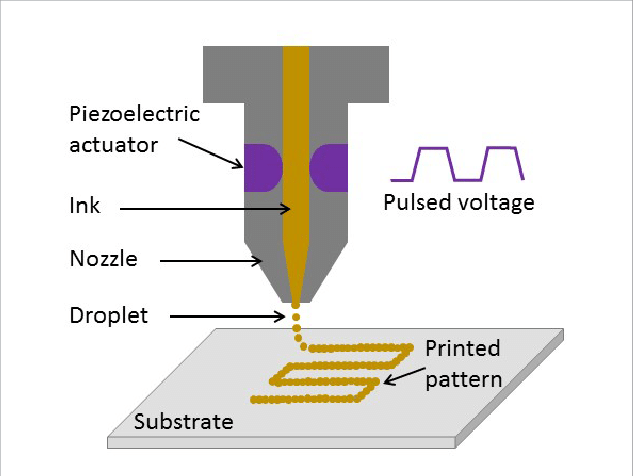
\includegraphics[width=0.5\linewidth]{Sections/2 Problemanalyse/Media/inkjet.png}
    \caption{Illustration af hvordan en Inkjet printer fungere \parencite{Long2025AOptimizations}}
    \label{fig: Inkjet}
\end{figure} \plainbreak{-0.5}

Inkjet-printere anvender dyser, der sprøjter væske ud som små dråber. Størrelsen på disse dråber og afstanden mellem dem bestemmes af både dysens udformning og systemets præstationsniveau, se figur \ref{fig: Inkjet}. Printhovedet kan tilpasses til at håndtere forskellige væsketyper, hvilket gør teknologien fleksibel i forhold til materialevalg. Systemet er primært designet til at arbejde på plane eller næsten plane overflader, da det kræver en ensartet afstand mellem printhovedet og emnet for at sikre korrekt afsætning af materialet.\parencite{Delaney2009InkjetProteins} 

Inkjet-printers bevægelsessystemer er karakteriseret ved høj nøjagtighed og genskabelighed, hvilket gør dem velegnede til opgaver, hvor præcis materialepositionering er nødvendigt. Systemet er ofte simpelt opbygget og kan tilpasse forskellige størrelser afhængigt af anvendelsen. Selvom inkjet-printere ofte anvendes til at printe tekst eller billeder på papir, kan teknologien også tilpasses andre formål, hvor præcis placering af små dråber eller partikler er nødvendigt.

%De andre printerteknologier, laser og termisk, kan allerede nu kasseres da laserprintere vil varme emnet op, og dermed kan ændre emnets egenskaber og termiske printer kun virker da papiret er varmereaktivt. De er derfor ikke relevante.

\textbf{FDM 3D Printere} bruges ofte med et standard kartesisk bevægelsessystem.  Det kartesiske bevægelsessystem for 3D-printeren er kendetegnet ved, at elmotorer kontrollerer bevægelse langs tre akser, x-, y- og z aksen, se figur \ref{fig:3D printer}.

\begin{figure} [H]
    \centering
    \includegraphics[width=0.5\linewidth]{Sections/2 Problemanalyse/Media/3D printer bevægelse.png}
    \caption{3D printer illustration. \parencite{Mueller20203DDraft}. }
    \label{fig:3D printer}
\end{figure}\plainbreak{-0.5}

 De er ofte lavet med bælter eller med en ledeskrue der kan føre printerhovedet i de tre retninger. Dette vil også være en mulig måde at lave en robotbevægelse, til påføring af speckle patterns, på en 2D overflade. \parencite{Billington20243DOverview}
\plainbreak{1} \input{Sections/2 Problemanalyse/4.2 Robotbevægelser}


\chapter{Problemformulering}
Speckle patterns er essentielle ved brugen af DIC til måling af materialeegenskaber. Tilgængelige metoder til påføring af speckle patterns på overflader er enten manuelle og tidskrævende, eller laver prikker der ikke er optimale til DIC. Robotter anvendes blandt andet til automatisering og effektivisering i fremstillingsindustrien, hvor de indgår som led i produktionen. På baggrund heraf er følgende problemformulering udformet:


\begin{displayquote} 
\large
\centering
    \textit{Hvordan designes en robot til påføring af speckle patterns i makroskala, på et plan i 2D, der kan anvendes ved Digital Image Correlation?}
\end{displayquote}


\section{Afgrænsning} \label{Afgrænsning}
Projektet afgrænses ud fra et ønske om at fokusere på studierelavanter afspekter af løsningsudviklingen. Det er valgt, at udelade design og udvikling af elektriske kredsløb og styringssystemer, samt programmering af robotten fra projektets omfang. Selvom der afgrænses fra udviklingen af de elektroniske aspekter af løsningen tages der stadig højde for, at de skal være inkluderet. Eksempelvis placering af styringsenheden. 

Det er bekendt, at farvemidlet til påføring af speckle patterns påvirker materialer på forskellige måder. Farvemidlers kemiske opbygning og fremstilling er udenfor studiets fagområde, og undersøges ikke i dette projekt.
%Dette valg sikrer, at fokusset udelukkende ligger på de mekaniske komponenter og de udfordringer, der er forbundet med deres design og funktion.

%Ved at holde projektet fokuseret på de mekaniske dele bliver omfanget både klart defineret og håndterbart. Denne afgrænsning giver mulighed for at foretage en dybdegående analyse og udvikling af de mekaniske systemer, uden at blive hindret af de elektriske og kemiske aspekter. Resultatet er en mere målrettet indsats, hvor der kan optimeres de mekaniske løsninger med den nødvendige præcision og kvalitet.

I dette projekt forstås 2D planer som kontinuerlige planer uden krumning.

\chapter{Kravspecifikation} \label{Kravspecifikation}

Kapitlet har til formål, at identificere potentielle kunders ønsker og krav, til en løsning der kan påføre speckle patterns i makroskala, til brug ved DIC. Der differentieres mellem ufravigelige krav og præstationskrav. Løsningen skal overholde de ufravigelige krav, for at den er brugbar. Fra problemformuleringen bliver følgende ufravigelige krav opstillet:
\begin{itemize}
    \item Materialets egenskaber må ikke ændres mere end 1\% efter tilføjelse af speckle pattern (\ref{Optimale speckle patterns}).
    \item Prikker skal deformerer med test-emnet (\ref{Optimale speckle patterns}).
    \item Løsningen skal producere et speckle pattern, der kan anvendes til DIC (\ref{Speckle pattern}).
    \item Løsningen skal kunne placere prikker på en 2D plan overflade (\ref{Afgrænsning}). 
    \item Løsningen skal være en robot (\ref{Robotter}).
\end{itemize}

Præstationskrav har en optimeringsretning, og behøver ikke at være opfyldt for løsningen er funktionel. Løsningen ønskes at have flere eller alle præstationskrav opfyldt, idet præstationskrav baseres på kunders ønsker, øger konkurrencedygtigheden af den endelige løsning. Præstationskravene udarbejdes gennem House of Quality (HoQ).

%Præstationskravene er krav, som ikke er strengt nødvendige for at produktet virker, men derimod konkurrence punkter.
\plainbreak{2}
\section{House of Quality} \label{House of Quality}
HoQ er et værktøj der benyttes i produktudvikling, til at identificere kunders ønsker og krav til den færdige løsning \parencite{Ullman2018TheProcess}. Det skal sikre, at centrale krav identificeres tidligt i processen og omsættes til målbare tekniske parametre, der kan danne grundlag for en struktureret og velbegrundet udviklingsproces. HoQ er opbygget af 8 trin der er illustreret i figur \ref{fig: HOQ illustration}.  

Udarbejdelsen af et HoQ begynder med trin 1, og fortsætter trin for trin. Udover at identificere kundens ønsker og dertilhørende designspecifikationer, skabes der i trin 6 og 8 indsigt i deres indbyrdes sammenhænge og relationer. Dette tydeliggør de designspecifikationer der er vigtigst at fokusere på, samt eventuelle konflikter eller afhængigheder i designet. Det betyder, at ændringen af én designspecifikation kan have indvirkning på en anden designspecifikation. 

\begin{figure}[H]
    \centering
    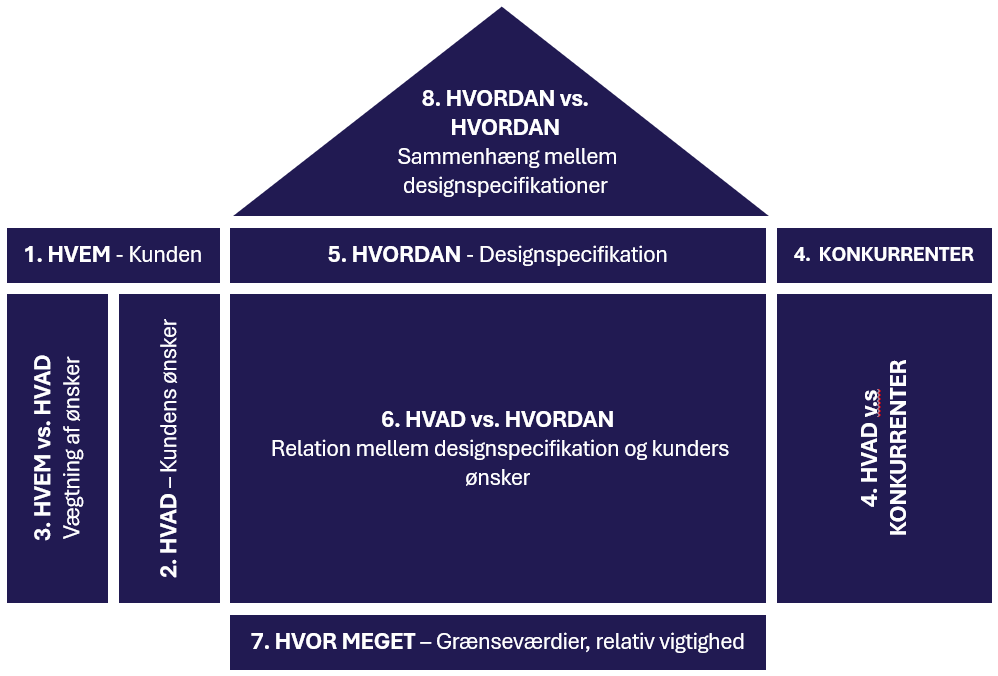
\includegraphics[width=1\linewidth]{Sections/4 Kravspecifikation/Media/HOQ1.png}
    \caption{Illustration af et House of Quality}
    \label{fig: HOQ illustration}
\end{figure} \plainbreak{-0.5}

En væsentlig fordel ved anvendelsen af HoQ er, at metoden bidrager til struktur og systematik i komplekse udviklingsforløb, hvor flere krav og tekniske hensyn skal afvejes. Metoden sikrer desuden en høj grad af klarhed i forhold til, hvordan de opstillede krav afspejles i de valgte designløsninger.



\begin{comment}
\begin{enumerate} 
    \item \textbf{Hvem} - Identifikation af kunder. \\
    \vspace{-0.4cm} \item \textbf{Hvad} - Identifikation af kunders ønsker. \\
    \vspace{-0.4cm} \item \textbf{Hvem vs. hvad} - Vægtning af kundernes ønsker.\\
    \vspace{-0.4cm} \item \textbf{Konkurrenter} - Undersøgelse og evaluering af konkurrenter. \\
    \vspace{-0.4cm} \item \textbf{Hvordan} - Udarbejdelse af designspecifikationer.\\
    \vspace{-0.4cm} \item \textbf{Hvad vs. hvordan} - Relationer mellem designspecifikationer og kundernes ønsker. \\
   \vspace{-0.4cm} \item \textbf{Hvor meget} - Udarbejdelse af grænseværdier for designspecifikationer.\\
\vspace{-0.4cm} \item \textbf{Hvordan vs. hvordan} - Identifikation af designspecifikationernes gensidige afhængighed. \\
\end{enumerate}
\end{comment}

%Processen indledes typisk med en systematisk identifikation af de krav, der vurderes at være væsentlige for det pågældende projekt. Disse krav kan eksempelvis omfatte funktionelle egenskaber, krav til præcision, ydeevne eller andre tekniske specifikationer, der har afgørende betydning for systemets eller produktets samlede funktionalitet. Efterfølgende prioriteres kravene på baggrund af deres betydning, hvorefter de oversættes til konkrete designparametre, som skal sikre opfyldelsen af de ønskede egenskaber.

%HoQ giver et struktureret og visuelt overblik i form af en matrix, hvor relationerne mellem krav og tekniske løsninger tydeliggøres og analyseres. Yderligere skabes der indsigt i, hvordan de tekniske løsninger påvirker hinanden indbyrdes, hvilket muliggør en tidlig identifikation af eventuelle konflikter eller afhængigheder i designet. Herved styrkes beslutningsgrundlaget for udviklingsteamet, som kan foretage prioriteringer med udgangspunkt i en helhedsorienteret vurdering af projektets krav og mål.

%Sammenfattende er HoQ et redskab til at strukturere og kvalificere beslutningsprocesser i projekter, hvor der stilles krav om høj funktionalitet, kvalitet og ydeevne. Metoden giver et solidt fundament for at sikre, at centrale krav bliver integreret i designet, og at de tekniske løsninger udvælges på et velunderbygget grundlag.


\plainbreak{2}
\subsection{Trin 1, 2, 3 og 4 - Identifikation af kunder, ønsker, vægtning og konkurrenter} \label{Trin 1-4}

\textbf{Trin 1} har til formål, at identificerer kunder og interessenter. I dette projekt, er der ingen konkret kunde, så i de følgende trin er kunders ønsker og vægtninger baseret på kapitel \ref{Problemanalyse} Problemanalyse. 
 
\textbf{Trin 2} identificerer kunders ønsker på baggrund af problemanalysen, ved vurdering af, hvad potentielle kunder vægter relevant for en speckle pattern robot. De identificerede ønsker kan ses i tabel \ref{tab: trin 1 til 4} sammen med vægtningen af de enkelte ønsker, som kommer fra trin 3. 

\textbf{Trin 3} vurderer kundens ønsker i forhold til, hvor vigtigt de antages at være baseret på problemanalysen (\ref{Problemanalyse}). Vægtningerne er lavet ved at fordele 100 point mellem de ti ønsker, hvor vigtigere ønsker får tildelt flere point, og mindre vigtige ønsker får tildelt færre point. At begrænse vægtningen til et total på 100 point tvinger en prioritering af ønskerne. 

\renewcommand{\arraystretch}{1.4}
\begin{table}[H]
    \caption{Vægtning af ønsker ved fordeling af 100 point. Vurdering af hvor godt konkurrenter opfylder kundernes ønsker fra fra 0 til 5. 0 = Opfylder overhovedt ikke ønsket, 1 = Minimal opfyldelse af ønsket, 2 = Lille opfyldelse af ønsket, 3 = Tildels opfyldelse af ønsket, 4 = Stor opfyldelse af ønsket og 5 = Fuldstændig opfyldelse af ønsket.}
    \centering
    \begin{tabular}{|l|c||c|c|c|c|} \cline{3-6}\cline{3-6}
    %Konkurrenter
        \multicolumn{2}{c|}{} & \rotatebox{90}{\hspace{-.3cm} \cellcolor{lightgray!20} \textbf{Stempel ruller}} & \rotatebox{90}{\hspace{-.3cm} \cellcolor{lightgray!20} \textbf{Tusch / tegneredskab}}  & \rotatebox{90}{\hspace{-.2cm} \cellcolor{lightgray!20}\textbf{Spraymaling}} & \rotatebox{90}{\hspace{-.3cm} \cellcolor{lightgray!20} \textbf{Midlertidig tatovering} \hspace{.2cm}}\\ 
         
    % Header med Ønsker og vægtning
      \multicolumn{1}{|c}{\cellcolor{aaublue} \textcolor{white}{\textbf{Ønsker}}} & \multicolumn{1}{|c}{\cellcolor{aaublue} \textcolor{white}{\textbf{Vægtning}}} & \multicolumn{4}{|c|}{\cellcolor{aaublue} \textcolor{white}{\textbf{Konkurrenter}}} \\ \specialrule{0pt}{0.5pt}{0pt} \hline 

    %værdier
        1. Producere et godt speckle pattern & 20 & 4 & 3 & 2 & 4\\ \hline
        2. Genskabelighed & 11 & 3 & 0 & 0 & 4 \\ \hline
        3. Håndtere forskellige emnestørrelser og former & 14 & 4 & 5 & 4 & 4 \\ \hline
        4. Håndtere forskellige materialer & 12 & 4 & 4 & 4 & 4 \\ \hline
        5. Hurtig fremstilling af speckle pattern & 10 & 4 & 1 & 5 & 3\\ \hline
        6. Brugervenlighed & 8 & 4 & 5 &3 & 3\\ \hline
        7. Lang levetid & 4 & 4 &1 & 1 & 0\\ \hline
        8. Lav arbejdsbyrde & 14 & 3 & 0 & 3 & 3\\ \hline
        9. Lav førstegangspris & 3 & 1 & 5 & 4 & 2\\ \hline
        10. Lav brugspris & 4 & 3 & 4 & 4 & 3 \\ \hline \specialrule{0pt}{0.8pt}{0pt} \cline{2-6}
        \multicolumn{1}{r|}{\textbf{SUM}} & 100 & 34 & 28 & 30 & 29 \\ \cline{2-6}
    \end{tabular}
    \label{tab: trin 1 til 4}
\end{table} \plainbreak{-0.5}

Det vurderes, at det vigtigste ønske, er ønske 1, om at producere et godt speckle pattern, fordi nøjagtigheden af DIC afhænger af kvaliteten af det anvendte speckle pattern, som det fremgår af afsnit \ref{Speckle pattern}. 

Ønske 3 om håndtering af forskellige emnestørrelse og former, samt ønske 8 om lav arbejdsbyrde tildeles begge 14 point, og er de næstvigtigste ønsker, fordi nuværende metoder til fremstilling af speckle pattern i makroskala, kræver at en person er manuelt involveret under det meste af processen. Det ses derfor som et konkurrencepunkt hvis arbejdsbyrden og tiden kan nedsættes ved automatisering af en robot. På baggrund af afsnit \ref{Fremstilling af Speckle pattern} har ønske 4 om at håndtere forksellige materialer fået 12 point. Dette er grundet DIC i dag anvendes på mange forskellige emnestørrelser og materialer, så det er fordelagtigt, hvis løsningen ikke er begrænset til en enkelt emnestørrelse eller materiale. 

De sidste ønsker, som ikke er nævnt, har en mindre vægtning. De er derfor ikke lige så relevante som de nævnte ønsker, og deres vægtning bliver dermed ikke forklaret yderligere. Alle vægtningerne kan ses i figur \ref{tab: trin 1 til 4}.


\textbf{Trin 4} ses til højre i tabel \ref{tab: trin 1 til 4}, hvor konkurrenterne vurderes på baggrund af ønskerne. Vurderingen af konkurrenter sker, for at identificerer ønsker, hvor der er mulighed for at skabe konkurrencepunkter. Fra afsnit \ref{Fremstilling af Speckle pattern} er stempel ruller, tusch/tegneredskab, spraymaling og midlertidig tatovering valgt som konkurrenter. Disse vægtes på en skala fra 0 til 5: %, disse kan ses i tabel \ref{...}:


\newcommand{\myhash}{\raisebox{\depth}{\#}}
\begin{enumerate}[font=\bfseries]\addtocounter{enumi}{-1}
    \item Opfylder overhovedet ikke ønsket 
    \item Minimal opfyldelse af ønsket 
    \item Lille opfyldelse af ønsket 
    \item Tildels opfyldelse af ønsket 
    \item Stor opfyldelse af ønsket 
    \item Fuldstændig opfyldelse af ønsket 
\end{enumerate}


Vurdering af konkurrenterne sker på baggrund af afsnit \ref{Fremstilling af Speckle pattern} i problemanalysen. Stempelruller og midlertidig tatoveringer får begge 4 point i ønske 1, hvor de øvrige får mindre. Dette betyder, at en endelig løsning helst skal have $\geq 4$, medmindre løsningen excellerer på andre områder, fordi ønsket har fået 20 point. Konkurrenterne får henholdsvis 3, 0, 3 og 3 point i ønske 8 om lav arbejdsbyrde, som er det ønske der vægtes anden højest. Det vurderes derfor, at lav arbejdsbyrde er et af de områder, som en løsningen kan differentiere sig fra konkurrenterne på. Det forventes at førstegangsprisen og brugsprisen af en robot som løsning, overstiger både tuscher og spraymaling. Løsningen vil stadig have markedspotentiale, da disse ønsker er vurderet lavest. 

 



\begin{comment}
Tidligere tabeller:

  \begin{table}[H]
    \caption{Vægtede ønsker}
    \centering
    \begin{tabular}{|l|c|}\hline
     \multicolumn{1}{|c}{\cellcolor{aaublue} \textcolor{white}{\textbf{Ønsker}}} &  \multicolumn{1}{|c}{\cellcolor{aaublue} \textcolor{white}{\textbf{Vægtning (ud af 100)}}} \\ \specialrule{0pt}{0.5pt}{0pt} \hline 
        1. Producere et godt speckle pattern & 20 \\ \hline
        2. Genskabelighed & 11\\ \hline
        3. Håndtere forskellige emnerstørrelser og former & 13 \\ \hline
        4. Håndtere forskellige materialer & 13 \\ \hline
        5. Hurtig fremstilling af speckle pattern & 10\\ \hline
        6. Brugervenlighed & 8\\ \hline
        7. Lang levetid & 4\\ \hline
        8. Lav arbejdsbyrde & 14 \\ \hline
        9. Lav førstegangspris & 3\\ \hline
        10. Lav brugspris & 4\\ \hline
    \end{tabular}
    \label{tab:vægønsker}
\end{table} 



\begin{table}[H]
    \centering
    \caption{Kundens vurdering af konkurrenternes produkter}
    \renewcommand{\arraystretch}{1.3} 
    \setlength{\tabcolsep}{8pt} 
    \begin{tabular}{|l|c|c|c|c|c|c|c|c|c|c||c|}
        \hline
        \rowcolor{lightgray!20} \cellcolor{aaublue}\textcolor{white}{ \textbf{ Ønske nr.}} & \textbf{1} & \textbf{2} & \textbf{3} & \textbf{4} & \textbf{5} & \textbf{6} & \textbf{7} & \textbf{8} & \textbf{9} & \textbf{10} & \textbf{sum} \\ \hline 
        \specialrule{0pt}{0.5pt}{0pt} \hline 
        
        \multicolumn{1}{|l|}{\cellcolor{aaublue} \textcolor{white}{\textbf{Stempel ruller}}} & 4 & 3 & 4 & 4 & 4 & 4 & 4 & 3 & 1 & 3 & 34 \\ 
        \hline
         \multicolumn{1}{|l|}{\cellcolor{aaublue} \textcolor{white}{\textbf{tusch / tegneredskab}}} & 3 & 0 & 5 & 4 & 1 & 5 & 1 & 0 & 5 & 4 & 28 \\ 
        \hline
        \multicolumn{1}{|l|}{\cellcolor{aaublue} \textcolor{white}{\textbf{Spraymaling}}} & 2 & 0 & 4 & 4 & 5 & 3 & 1 & 3 & 4 & 4 & 30 \\ 
        \hline
        \multicolumn{1}{|l|}{\cellcolor{aaublue} \textcolor{white}{\textbf{Midlertidig tatovering}}}  & 4 & 4 & 4 & 4 & 3 & 3 & 0 & 3 & 1 & 3 & 29 \\ 
        \hline
    \end{tabular}
    \label{Tab: Kunde vs. konk.}
\end{table}


\begin{table}[H]
    \caption{Vægtede ønsker fra 0 til 100}
    \centering
    \begin{tabular}{|l|c | p{.1pt}|c|c|c|c|} \cline{4-6}\cline{4-7}
    %Konkurrenter
        \multicolumn{3}{c|}{}  & \rotatebox{90}{\hspace{-.3cm} \cellcolor{lightgray!20} \textbf{Stempel ruller}} & \rotatebox{90}{\hspace{-.3cm} \cellcolor{lightgray!20} \textbf{tusch / tegneredskab}}  & \rotatebox{90}{\hspace{-.2cm} \cellcolor{lightgray!20}\textbf{Spraymaling}} & \rotatebox{90}{\hspace{-.2cm} \cellcolor{lightgray!20}\textbf{Midlertidig tatovering}}\\ 
         
    % Header med Ønsker og vægtning
      \multicolumn{1}{|c}{\cellcolor{aaublue} \textcolor{white}{\textbf{Ønsker}}} & \multicolumn{1}{|c}{\cellcolor{aaublue} \textcolor{white}{\textbf{Vægtning}}} & ~ & \multicolumn{4}{|c|}{\cellcolor{aaublue} \textcolor{white}{\textbf{Konkurrenter}}} \\ \specialrule{0pt}{0.5pt}{0pt} \cline{1-2} \cline{4-7}

    %værdier
        1. Producere et godt speckle pattern & 20 & ~ &  4 & 3 & 2 & 4\\ \cline{1-2} \cline{4-7}
        2. Genskabelighed & 11 & ~ & 3 & 0 & 0 & 4 \\ \cline{1-2} \cline{4-7}
        3. Håndtere forskellige emnerstørrelser og former & 13 & ~ & 4 & 5 & 4 & 4 \\ \cline{1-2} \cline{4-7}
        4. Håndtere forskellige materialer & 13 &  ~& 4 & 4 & 4 & 4 \\ \cline{1-2} \cline{4-7}
        5. Hurtig fremstilling af speckle pattern & 10 &  ~& 4 & 1 & 5 & 3\\ \cline{1-2} \cline{4-7}
        6. Brugervenlighed & 8 &  ~& 4 & 5 &3 & 3\\ \cline{1-2} \cline{4-7}
        7. Lang levetid & 4 & ~ & 4 &1 & 1 & 0\\ \cline{1-2} \cline{4-7}
        8. Lav arbejdsbyrde & 14 &  ~&3 & 0 & 3 & 3\\ \cline{1-2} \cline{4-7}
        9. Lav førstegangspris & 3 & ~ & 1 & 5 & 4 & 2\\ \cline{1-2} \cline{4-7}
        10. Lav brugspris & 4 & ~ & 3 & 4 & 4 & 3 \\ \cline{1-2} \cline{4-7} \specialrule{0pt}{0.8pt}{0pt} \cline{4-7}
        \multicolumn{3}{r|}{\textbf{SUM}}  & 34 & 28 & 30 & 29 \\ \cline{4-7}
    \end{tabular}
    \label{tab: trin 1 til 4}
\end{table}
\end{comment} \plainbreak{2}
\subsection{Trin 5 - Udarbejdelse af designspecifikationer} \label{Trin 5}
Det femte trin har til formål, at omsætte ønsker til målbare designspecifikationer, der muligører konkrete og målbare test af den endelige løsning. Designspecifikationerne beskrives i dette afsnit og kan ses i tabel \ref{tab:krav}.

\renewcommand{\arraystretch}{1.2}
\begin{table}[H]
    \centering
     \caption{Design specifikationer.For optimerings retningen (OR) betyder \textbf{--} en fastlagt værdi, \protect$\btdown$ betyder specifikationen forbedres når værdien mindskes og $\blacktriangle$ betyder specifikationen forbedres når værdien øges}
    \begin{tabular}{|l|c|c|} \hline
     \multicolumn{1}{|c}{\cellcolor{aaublue} \textcolor{white}{\textbf{Designspecifikation}}} &  \multicolumn{1}{|c}{\cellcolor{aaublue} \textcolor{white}{\textbf{Enhed}}} &  \multicolumn{1}{|c}{\cellcolor{aaublue} \textcolor{white}{\textbf{OR}}} \\ \specialrule{0pt}{0.5pt}{0pt} \hline 
        1. Prikstørrelse& mm & \textbf{--} \\ \hline
        2. Variation på prikstørrelser & mm & $\btdown$ \\ \hline
        3. Variation på prikplacering & mm & $\btdown$ \\ \hline
        4. Størrelse af arbejdsområdet & mm & $\blacktriangle$\\ \hline
        5. Flytning af emnet under fremstilling af speckle pattern & mm & $\btdown$\\ \hline
        6. Antal forskellige farvemidler til speckle pattern & Farvemidler & $\blacktriangle$ \\ \hline
        7. Kontrast mellem prik og baggrund	& -- & $\blacktriangle$ \\ \hline
        8. Tidsforbrug på prikplacering & $\SI{}{s/cm^2}$ & $\btdown$ \\ \hline
        9. Brugerinvolvering under process & min & $\btdown$\\ \hline
        10. Tid brugt på opsætning  & min & $\btdown$\\ \hline
        11. Antal værktøj til at samle hele produktet & Værktøj & $\btdown$ \\ \hline
        12. Antal specialværktøj til at samle hele produktet & Værktøj & $\btdown$\\ \hline
    \end{tabular}
    \label{tab:krav}
\end{table}

\textbf{1. Prikstørrelse} er valgt på baggrund af ønske 3 om forskellige emnestørrelser og former. Denne designspecifikation beskriver det spænd af prikstørrelser løsningen kan producere. 

\textbf{2. Variation på prikstørrelser} beskriver den acceptable afvigelse fra den valgte prikstørrelse. For at kunne producere et godt speckle pattern skal denne variation minimeres.

\textbf{3. Variation af prikplacering} beskriver den acceptable afvigelse fra den teoretiske placering og den virkelige placering. Dette er valgt på baggrund af den høje vægtning tildelt ønske 2 om genskabelighed. 

\textbf{4. Størrelse af arbejdsområdet} sættes som designspecifikation, fordi det skal være muligt, at sætte prikker på forskellige størrelser emner, som det fremgår af ønske 3. 

\textbf{5. Fastholdelse af emnet} sikrer et godt speckle pattern som der vægtes i ønske 1. Det er en nødvendighed, at emnet ikke bevæger sig under påføring, således robotten kan overføre det ønskede speckle pattern så præcist som muligt.

\textbf{6. Antal forskellige farvemidler til speckle pattern} skal sikre, at produktet kan skabe speckle patterns på alle emnematerialer ved at inkludere flere forskellige farvemidler, så farver og materialer altid fungere optimalt i forhold til det enkelte emne.

\textbf{7. Kontrast mellem prik og baggrund} er en nødvendighed for at have et godt speckle pattern, som der ønskes i ønske 1. Det beskriver forholdet i lysstyrke mellem prik og emnet.

\textbf{8. Tidsforbrug på prikplacering} kommer direkte fra ønske 5 om hurtig fremstilling af speckle patterns. 

\textbf{9. Brugerinvolvering under proces} specificeres som den mængde tid, brugeren skal bruge efter de har sat processen i gang. Dette skal minimeres for at opfylde ønske 6 samt 8. En løsning der kræver at brugeren observerer den under processen er ikke brugervenlig.
  
\textbf{10. Tid brugt på opsætning} er en faktor i ønske 6 og 8. Dette beskriver tiden brugt på at sætte processen i gang.

\textbf{11. Antal værktøj til at samle hele produktet} har en effekt på hvor intuitiv løsningen er at samle. For at lave produktet brugervenligt, ønskes antallet derved så lavt som muligt.

\textbf{12. Antal specialværktøj til at samle hele produktet} er til for at holde løsningen brugervenlig som mulig, da løsningen ikke skal blive unødvendigt krævende at sammensætte. Derfor fremsættes en øvre grænse for, hvor mange forskellige stykker specialværktøj, der må påkræves for at samle produktet.

\plainbreak{2}
\subsection{Trin 6 - Relationer mellem designspecifikationer og kundernes ønsker} \label{Trin 6}
I det 6. trin beskrives relationen mellem kundens ønsker og de udarbejdede designspecifikationer. Her er der givet henholdsvis 1 point for en lav relation $(\bigtriangledown)$, 3 point for en middel relation $(\bigcirc)$ og 9 point for en stærk relation $(\blackbigcirc)$.  Det efterstræbes at alle ønsker som minimum har én stærk relation til 2 designspecifikationer, som det ses i tabel 4.3 i trin 6. Herved sikres, at ønskerne er ligeligt repræsenteret i designspecifikationerne.

\begin{table}[H]
\centering
\caption{ Relation mellem ønsker og designspecifikationer. $\protect\blackbigcirc$ = stærk relation, $\bigcirc$ = moderat relation og $\bigtriangledown$ = svag relation.}
\label{fig: HOQ trin 6} 
\footnotesize
\def\arraystretch{2}
\begin{tabular}{|p{4.cm}|c|c|c|c|c|c|c|c|c|c|c|c|}
    \hline
    \cellcolor{aaublue} \textcolor{white}{\diagbox[height=6cm, width=4.4cm]{\raisebox{0.9\height}{\enspace \textbf{\large Ønsker}}}{\raisebox{-0.9\height}{\enspace \makecell{\textbf{\normalsize Design-} \\ \textbf{\normalsize Specifikationer}}}}} & \cellcolor{lightgray!20} \rotatebox{90}{\hspace{-2.9cm} 1. Prikstørrelse} & \cellcolor{lightgray!20} \rotatebox{90}{\hspace{-2.9cm} 2. Variation på prikstørrelse} & \cellcolor{lightgray!20} \rotatebox{90}{\hspace{-2.9cm} 3. Variation på prikplacering} & \cellcolor{lightgray!20} \rotatebox{90}{\hspace{-2.9cm} 4. Størrelse af arbejdsområde} & \cellcolor{lightgray!20} \rotatebox{90}{\hspace{-2.9cm} \makecell[l]{\addlinespace[-3pt] 5. FLytning af emnet under fremstilling \\ \quad af speckle pattern \vspace{-3pt} }} & \cellcolor{lightgray!20} \rotatebox{90}{\hspace{-2.9cm} \makecell[l]{\addlinespace[-3pt] 6. Antal forskellige farvemidler til \\ \quad speckle pattern \vspace{-3pt}}} & \cellcolor{lightgray!20} \rotatebox{90}{\hspace{-2.9cm} \makecell[l]{\addlinespace[-3pt] 7. Kontrast mellem prik og baggrund \vspace{-3pt} }} & \cellcolor{lightgray!20} \rotatebox{90}{\hspace{-2.9cm} 8. Tidsforbrug på prikplacering} &\cellcolor{lightgray!20} \rotatebox{90}{\hspace{-2.9cm} 9. Brugerinvolvering under process} & \cellcolor{lightgray!20} \rotatebox{90}{\hspace{-2.9cm} 10. Tid brugt på opsætning} & \cellcolor{lightgray!20} \rotatebox{90}{\hspace{-2.9cm} \makecell[l]{\addlinespace[-3pt] 11. Antal værktøj til at samle hele \\ \quad produktet }} & \cellcolor{lightgray!20} \rotatebox{90}{\hspace{-2.9cm} \makecell[l]{\addlinespace[-3pt] 12. Antal specialværktøj til at samle \\ \quad hele produktet \vspace{-3pt} }}  \\
    \hline
     \cellcolor{lightgray!20} \makecell[l]{\addlinespace[0pt] 1. Producere et godt \\ \quad speckle pattern \vspace{0pt}} & $\bigcirc$ & $\blackbigcirc$ & $\blackbigcirc$ & & $\blackbigcirc$  &  & $\bigcirc$ &  & & & & \\
    \hline
    \cellcolor{lightgray!20} 2. Genskabelighed & $\bigtriangledown$& $\blackbigcirc$ & $\blackbigcirc$ & & $\blackbigcirc$& & & & & &&\\
    \hline
    \cellcolor{lightgray!20} \makecell[l]{\addlinespace[0pt] 3. Håndtere forskellige \\ \quad objekt størrelser og former} \vspace{-10pt}  & $\blackbigcirc$& & & $\blackbigcirc$ &$\bigcirc$& & &$\bigcirc$& & & &\\
    \hline
    \cellcolor{lightgray!20} \makecell[l]{\addlinespace[0pt] 4. Håndtere forskellige \\ \quad materialer} \vspace{0pt} & & & & & $\bigcirc$ & $\blackbigcirc$& $\blackbigcirc$ & & & & & \\
    \hline
    \cellcolor{lightgray!20} \makecell[l]{\addlinespace[0pt]  5. Hurtig fremstilling af \\ \quad speckle pattern} \vspace{0pt} & $\bigcirc$& $\bigtriangledown$&$\bigtriangledown$& $\bigcirc$ & & &  & $\blackbigcirc$ & $\bigcirc$ & $\blackbigcirc$& & \\
    \hline
    \cellcolor{lightgray!20} 6. Brugervenlighed && & & & & & & & $\bigtriangledown$& $\bigcirc$ & $\blackbigcirc$ & $\blackbigcirc$ \\
    \hline
    \cellcolor{lightgray!20} 7. Lang levetid & & & & & & $\bigcirc$ & & $\bigtriangledown$& & &$\blackbigcirc$& $\bigcirc$ \\
    \hline
    \cellcolor{lightgray!20} 8. Lav arbejdsbyrde & & & & & & & & & $\blackbigcirc$ & $\blackbigcirc$ & $\bigcirc$& $\bigcirc$\\
    \hline
    \cellcolor{lightgray!20}  9. Lav førstegangspris&$\bigcirc$& $\bigcirc$& $\bigcirc$& $\bigcirc$& &$\bigcirc$ & & $\blackbigcirc$& & & & $\blackbigcirc$ \\
    \hline
    \cellcolor{lightgray!20} 10. Lav brugspris& & & & & & $\blackbigcirc$ & & & $\bigcirc$& $\blackbigcirc$& &  \\
    \hline
\end{tabular}
\end{table} \plainbreak{-0.5}

Relationer mellem ønsker og designspecifkationer kan være positive, såvel som negative. Design specifikation 2 og 3 for eksempel har en positiv relation med ønsket om genskabelighed, men en negativ relation med ønsket om lav førstegangspris. For at skabe en høj genskabelighed skal produktet have en høj nøjagtighed. En forøgelse af nøjagtighed (og dermed lavere tolerancer) kommer ofte også med en højere pris. Dermed modstrider disse ønsker hinanden. Dette uddybes i afsnit \ref{Trin 8}.
\plainbreak{2}
\subsection{Trin 7 - Udarbejdelse af grænseværdier for designspecifikationer} \label{Trin 7} 

Designspecifikationer er målbare krav, med en optimerings retning og en grænseværdi. Grænseværdierne opstilles for designspecifikationerne fra tabel \ref{tab:krav}, på baggrund af problemanalysen i kapitel \ref{Problemanalyse}. Løsninger der ligger udenfor én eller flere af grænseværdierne, er ikke konkurrencedygtige på de punkter, men er stadig funktionelle løsninger.

Designspecifikation 1 har ingen optimeringsretning, fordi den har en øvre og en nedre grænse. Den nedre grænse er en hård grænse da løsningen vil bevæge sig ind i mikroskala-området hvis den kommer under. Den beskrives som en designspecifikation, da en løsning der kun kan producere prikker mellem \(\SI{0,1}{mm}\) og \(\SI{0,5}{mm}\) stadig er en funktionel løsning, men den mister konkurrencedygtighed. Herunder sættes værdier og enheder på designspecifikationerne.

%Designspecifikation 1 er unik i forhold til de andre da den ingen optimeringsretning har, og reelt består af 2 forskellige værdier, en øvre og nedre grænse. 

%For designspecifikation 1 er den ønskede specifikation angivet til mellem 0,1 og 1. Der er ingen optimeringsretning, idet prikstørrelsen skal være valgbar indenfor det ønskede interval. Der er afgrænset til makroskala, hvorfra grænseværdien er $\leq 0.1$ mm, som angiver grænsen mellem mikro- og makroskala. Et produkt der producerer prikker på mikroskala opfylder ikke kravet om makroskala, og kan derfor ikke anvendes til det ønskede formål. Der opstilles ønskede specifikationer for alle designspecifikationer, som ses i tabel \ref{tab:trin 7 designspec}.  


\begin{table}[H]
    \centering
     \caption{Design specifikationer. For optimerings retningen (OR) betyder \textbf{--} en fastlagt værdi, \protect$\btdown$ betyder specifikationen forbedres når værdien mindskes og $\blacktriangle$ betyder specifikationen forbedres når værdien øges. Relativ vigtighed ($\Omega$)}
      \begin{tabular}{|l|c|c|c|c|} \hline
     \multicolumn{1}{|c}{\cellcolor{aaublue} \textcolor{white}{\textbf{Designspecifikation}}} & \multicolumn{1}{|c}{\cellcolor{aaublue} \textcolor{white}{\textbf{OR}}} &\multicolumn{1}{|c}{\cellcolor{aaublue} \textcolor{white}{\textbf{Grænseværdi}}} & \multicolumn{1}{|c}{\cellcolor{aaublue} \textcolor{white}{\textbf{Enhed}}} & \multicolumn{1}{|c|}{\cellcolor{aaublue} \textcolor{white}{$\Omega$}} \\ \specialrule{0pt} {0.5pt}{0pt} \hline
        1. Prikstørrelse & \textbf{--} & 0,1 og 1,0 & mm & 9\% \\ \hline
        2. Variation på prikstørrelser & $\btdown$ & $\pm0,05$& mm & 11\% \\ \hline
         3. Variation på prikplacering & $\btdown$ & $\pm0,1$ & mm & 11\% \\ \hline
        \makecell[l]{4. Størrelse af arbejdsområde \\ \quad  speckle pattern} & $\blacktriangle$ & $200 \times 150 \times 50 $ & mm & 6\% \\ \hline
        \makecell[l]{5. Flytning af emnet under fremstilling \\ \quad  af speckle pattern}  & $\btdown$ & 0,01 & mm & 13\% \\ \hline
        \makecell[l]{6. Antal forskellige farvemidler til \\ \quad  spceckle pattern} & $\blacktriangle$ & 2 & \small Farvemidler & 6\% \\ \hline
        \makecell[l]{7. Kontrast mellem prik og baggrund} & $\blacktriangle$ & 100 & - & 7\% \\ \hline
        8. Tidsforbrug på prikplacering & $\btdown$ & 30 & $\SI{}{s/cm^2}$ & 6\%\\ \hline
        \makecell[l]{9. Brugerinvolvering under process} & $\btdown$ & 1 & min & 9\% \\ \hline
        10. Tid brugt på opsætning  & $\btdown$  & 10 & min & 10\% \\ \hline
        \makecell[l]{ 11. Antal værktøj til at samle hele  \\ \quad \,produktet} & $\btdown$ & 5 & \small Værktøj & 6\%\\ \hline
        \makecell[l]{12. Antal specialværktøj til at samle \\ \quad \, hele produktet} & $\btdown$ & 1 & \small Værktøj & 6\%\\ \hline
    \end{tabular}
    \label{tab:trin 7 designspec}
\end{table} \plainbreak{-0.8}

Sidste kolonne i tabel \ref{tab:trin 7 designspec} angiver designspecifikationens relative vigtighed ($\Omega$) i forhold til de øvrige designspecifikationer. Den relative vigtighed beregnes ved først at gange sammenhængen mellem ønsker og den enkelte designspecifikation (kolonnerne i tabel \ref{fig: HOQ trin 6}) med vægtningen af hvert ønske i trin 3. Den relative vigtighed beregnes ved formel \ref{formel: relativ vigtighed}, hvor point fra en enkelt designspecifikations relation til alle ønsker noteres med det græske tegn $\beta$. $\beta$ er summen af vægtninger ($\nu$) ganget med relationens værdi ($\psi$).
\begin{equation} \label{formel: relativ vigtighed}
    \Omega = \frac{\sum(\nu\cdot \psi)}{\sum(\sum(\nu\cdot \psi)} = \frac{\beta}{\sum\beta}
\end{equation}

Fra afsnit \ref{Trin 6} er det opgivet, at en stærk relation ($\blackbigcirc$) = 9 point, moderat relation ($\bigcirc$) = 3 point og en svag relation ($\bigtriangledown$) = 1 point. For hver designspecifikation ganges værdien fra relationen med det relaterede ønskes vægtning. 



\begin{comment}
Dette giver point for relationen per designspecifiktation ($\textnormal{Point}_\textnormal{{Rpd}}$)  Dette er beskrevet i formel \ref{formel: Point fra relation}, hvor 

\begin{equation} \label{formel: Point fra relation}
    \textnormal{Point}_\textnormal{{Rpd}}= \sum \textnormal{vægtning} \cdot\ \textnormal{relations værdi}
\end{equation}

Den relative vigtighed af hver design specifikation er procenten den udgør af den summen af alle $\textnormal{Point}_\textnormal{{Rpd}}$, som det ses i formel \ref{formel: Relativ vigtighed}:

\begin{equation} \label{formel: Relativ vigtighed}
    \textnormal{Relativ vigtighed} = \frac{\textnormal{Point}_{\textnormal{Rpd}}}{\sum \textnormal{Point}_{\textnormal{Rpd}}}
\end{equation}


Gamle tabel:
\begin{table}[H]
    \centering
     \caption{Design specifikationer. For optimerings retningen (OR) betyder \textbf{--} en fastlagt værdi, $\btdown$ betyder specifikationen forbedres når værdien mindskes og $\blacktriangle$ betyder specifikationen forbedres når værdien øges. Relativ vigtighed ($\Omega$)}
      \begin{tabular}{|l|c|c|c|c|c|} \hline
     \multicolumn{1}{|c}{\cellcolor{aaublue} \textcolor{white}{\textbf{Designspecifikation}}} & \multicolumn{1}{|c}{\cellcolor{aaublue} \textcolor{white}{\textbf{OR}}} & \multicolumn{1}{|c}{\cellcolor{aaublue} \textcolor{white}{\textbf{Ønsket spec.}}} &\multicolumn{1}{|c}{\cellcolor{aaublue} \textcolor{white}{\textbf{Grænseværdi}}} & \multicolumn{1}{|c}{\cellcolor{aaublue} \textcolor{white}{\textbf{Enhed}}} & \multicolumn{1}{|c|}{\cellcolor{aaublue} \textcolor{white}{$\Omega$}} \\ \specialrule{0pt} {0.5pt}{0pt} \hline
        \makecell[l]{1. Prikstørrelse } & \textbf{--} & 0,1 - 1 & 1,2 & mm & 9\% \\ \hline
        2. Variation på prikstørrelser & $\btdown$ & 0 & 0,05& mm & 11\% \\ \hline
        3. Variation på prikplacering & $\btdown$ & 0 & 0,1 & mm & 11\% \\ \hline
        \makecell[l]{4. Størrelse af arbejdsområde \\ \quad  speckle pattern} & $\blacktriangle$ & $200 \times 150 \times 50 $ & $ \geq 150 \times 100 \times 20 $ &mm & 6\% \\ \hline
        \makecell[l]{5. Flytning af emnet under \\ \quad  fremstilling af speckle pattern}  & $\btdown$ & 0 & 0,01 & mm & 13\% \\ \hline
        \makecell[l]{6. Antal forskellige farvemidler \\ \quad til spceckle pattern} & $\blacktriangle$ & 3 &  $ \geq 1$& - & 6\% \\ \hline
        \makecell[l]{7. Kontrast mellem prik og \\ \quad  baggrund}	& $\blacktriangle$ & $< 130$ & 100 & - & 7\% \\ \hline
        \makecell[l]{8. Tidsforbrug på prikplacering } & $\btdown$ & 25 & 30 & $s/cm^2$ & 6\%\\ \hline
        \makecell[l]{9. Brugerinvolvering under \\ \quad  process} & $\btdown$ & 0 & 1 & min & 9\% \\ \hline
        10. Tid brugt på opsætning  & $\btdown$  & 2 & 10 & min & 10\% \\ \hline
       \makecell[l]{ 11. Antal værktøj til at samle \\ \quad \,  hele produktet} & $\btdown$ & 5 & 7 & - & 6\%\\ \hline
        \makecell[l]{12. Antal specialværktøj til \\ \quad \, at samle hele  produktet}  & $\btdown$ & 0 & 1 & - & 6\%\\ \hline
    
    \end{tabular}
    \label{tab:trin 7 designspec}
\end{table}
\end{comment}








\plainbreak{2}
\subsection{Trin 8 - Designspecifikationernes gensidige afhængighed} \label{Trin 8}

%- Vurderingen af hvordan optimering af en designspecifikation påvirker optimeringen af en anden designspecifikation. Derfor kan alle designspecifikation der ikke har en optimeringsretningen ikke vurderes mellem hinanden. 

\begin{comment}
  \begin{figure} [H]
    \centering
    \includegraphics[width=0.65\linewidth]{Sections/4 Kravspecifikation/Media/Tag til HoQ.jpg}
    \caption{Tag til HOQ}
    \label{fig:Tag til HOQ}
\end{figure}  
\end{comment}

Taget i et HoQ, som der kan se i figur \ref{Table: HOQ tag ny}, viser hvordan de forskellige designspecifikationer påvirker hinanden. Her markeres der, om en forbedring af en designspecifikation, også gavner et andet (\textcolor{ForestGreen}{$+$}), eller om det kan skabe en konflikt (\textcolor{red}{$-$}). For eksempel kan det ses, at høj hastighed gør det sværere at sikre høj præcision, og det bliver vist med et minus i taget. På den måde hjælper taget med at give overblik over, hvor der skal være fokus, når der træffes designbeslutninger. Det gør det lettere at finde de bedste løsninger, uden at skabe nye problemer andre steder.


\begin{figure}[H]
\centering
\begin{tikzpicture}[font=\small, myfit/.style={fill=white,draw,line width=\mylinewidth,
 inner sep=-0.5*\mylinewidth,fit=#1}, 
 ]
 \def\mylinewidth{1pt}
 \matrix[matrix of nodes, nodes={draw,line width=\mylinewidth,minimum width=1.6em,
 minimum height=1.4em, anchor=center}, column sep=-\mylinewidth,
 ,row sep=-\mylinewidth,%nodes in empty cells,
 column 1/.style={nodes={minimum width=9.4cm,minimum height=0.8cm}},
 column 2/.style={nodes={minimum width=0.8cm,minimum height=0.8cm}}]  (mat)
 { \hspace{-2.9cm} 1. Justering af prikstørrelse i makroskala  & $\textbf{--}$  &\\
 \hspace{-4.75cm} 2. Variation på prikstørrelse &  $\btdown$ &\\
     \hspace{-4.65cm} 3. Variation på prikplacering & $\btdown$ & \\
     \hspace{-4.65cm} 4. Størrelse af arbejdsområde  & $\blacktriangle$ & \\
     \hspace{-.25cm} 5. Flytning af emnet under fremstilling af speckle pattern &  $\btdown$ &\\
     \hspace{-1.4cm} 6. Antal forskellige farvemidler til speckle pattern & $\btdown$  & \\
     \hspace{-3.45cm} 7. Kontrast mellem prik og baggrund & $\blacktriangle$ & \\
     \hspace{-4.4cm} 8. Tidsforbrug på prikplacering &  $\blacktriangle$ &\\
     \hspace{-3.8cm} 9. Bruger involvering under proces & $\btdown$ &\\
     \hspace{-4.9cm} 10. Tid brugt på opsætning  & $\btdown$ & \\
     \hspace{-2.25cm} 11. Antal værktøj til at samle hele produktet &  $\btdown$ &\\
     \hspace{-1.1cm} 12. Antal specialværktøj til at samle hele produktet & $\btdown$ & \\
 };


\draw[line width=\mylinewidth] (13.35em,12.57em) -- (26em,0em);
\draw[line width=\mylinewidth] (13.35em,10.5em) -- (25em,-1.1em);
\draw[line width=\mylinewidth] (13.35em,8.4em) -- (24em,-2em);
\draw[line width=\mylinewidth] (13.35em,6.3em) -- (22.9em,-3.1em);
\draw[line width=\mylinewidth] (13.35em,4.2em) -- (21.8em,-4.2em);
\draw[line width=\mylinewidth] (13.35em,2.1em) -- (20.7em,-5.2em);
\draw[line width=\mylinewidth] (13.35em,0.em) -- (19.6em,-6.3em);
\draw[line width=\mylinewidth] (13.35em,-2.em) -- (18.59em,-7.3em);
\draw[line width=\mylinewidth] (13.35em,-4.2em) -- (17.57em,-8.3em);
\draw[line width=\mylinewidth] (13.35em,-6.3em) -- (16.56em,-9.35em);
\draw[line width=\mylinewidth] (13.35em,-8.3em) -- (15.55em,-10.4em);
\draw[line width=\mylinewidth] (13.35em,-10.4em) -- (14.5em,-11.5em);


\draw[line width=\mylinewidth] (13.35em,10.4em) -- (14.5em,11.5em);
\draw[line width=\mylinewidth] (13.35em,8.3em) -- (15.55em,10.4em);
\draw[line width=\mylinewidth] (13.35em,6.3em) -- (16.56em,9.35em);
\draw[line width=\mylinewidth] (13.35em,4.2em) -- (17.57em,8.3em);
\draw[line width=\mylinewidth] (13.35em,2.em) -- (18.59em,7.3em);
\draw[line width=\mylinewidth] (13.35em,0.em) -- (19.6em,6.3em);
\draw[line width=\mylinewidth] (13.35em,-2.em) -- (20.7em,5.2em);
\draw[line width=\mylinewidth] (13.35em,-4.2em) -- (21.8em,4.2em);
\draw[line width=\mylinewidth] (13.35em,-6.3em) -- (22.9em,3.1em);
\draw[line width=\mylinewidth] (13.35em,-8.4em) -- (24em,2em);
\draw[line width=\mylinewidth] (13.35em,-10.5em) -- (25em,1.1em);
\draw[line width=\mylinewidth] (13.35em,-12.57em) -- (26em,0em);


\begin{scope}
  \foreach \Coord in {(14.45em, 10.45em), (15.5em, 5.25em), (15.45em, 1.1em), (16.55em, 6.25em),(17.6em, 3.18em),(18.61em, 4.25em)}
  {\node[fill=ForestGreen, inner sep=7pt,rotate=45] at \Coord {};}
 \end{scope} 

\begin{scope}
  \foreach \Coord in {(14.45em, 10.45em), (15.5em, 5.25em), (15.5em, 1.1em), (16.57em, 6.25em),(17.65em, 3.15em),(18.72em, 4.15em)}
  {\node at \Coord {\color{black}\textbf{+}};}
 \end{scope} 

 \begin{scope}
  \foreach \Coord in {(14.45em, -10.45em), (17.6em, 1.1em), (18.65em, -2.15em) , (18.63em, 2.12em), (19.7em, 3.2em), (22.91em, 2.05em)}
  {\node[fill=red, inner sep=7pt,rotate=45] at \Coord {};}
 \end{scope} 
 
 \begin{scope}
  \foreach \Coord in {(14.45em, -10.45em), (17.65em, 1.1em), (18.65em, -2.15em) , (18.7em, 2.1em), (19.7em, 3.1em), (22.91em, 2.05em)}
  {\node at \Coord {\textbf{\color{black}\Large{--}}};}
 \end{scope} 

\end{tikzpicture}
\caption{Relation mellem designspecifikationer} 
\label{Table: HOQ tag ny}
\end{figure} \plainbreak{-0.5}


Der er flere faktorer i HoQ, der har en negativ sammenhæng med hastighed (tidsforbrug på prikplacering). For eksempel kan øget hastighed, gå ud over tolerancen i prikstørrelse, tolerancen i prikplaceringen og arbejdsområdet, hvor et større arbejdsområde vil få  processen til at tage længere tid. Det betyder, at hvis det ønskes at øge hastigheden, skal der være fokus på, at det kan have en negativ indvirkning på andre vigtige krav i designet. 





\begin{comment}
\begin{figure}[H]
\small
\centering
\begin{tikzpicture}[font=\small, myfit/.style={fill=white,draw,line width=\mylinewidth,
 inner sep=-0.5*\mylinewidth,fit=#1}, 
 circ/.style={path picture={\draw circle (0.3em);}},
 circdot/.style={path picture={\draw circle (0.3em); 
 \fill circle (0.1em);}},
 trian/.style={path picture={\draw (-30:0.3em) -- (90:0.3em) -- (210:0.3em) --cycle ;}},
 ]
 \def\mylinewidth{1pt}
 \matrix[matrix of nodes, nodes={draw,line width=\mylinewidth,minimum width=1.6em,
 minimum height=1.6em, anchor=center}, column sep=-\mylinewidth,
 ,row sep=-\mylinewidth, %nodes in empty cells,
 row 1/.style={nodes={minimum width=0.8cm,minimum height=0.8cm}},
 row 2/.style={nodes={ rotate=90, minimum width=9.4cm, minimum height=0.8cm}}](mat) 
 {
    & & & \textbf{--}  & $\btdown$ &  $\btdown$ & $\blacktriangle$ & $\btdown$ & $\blacktriangle$ & $\blacktriangle$  &$\btdown$ & $\btdown$ & $\btdown$  & $\btdown$&$\btdown$\\
    & &  & \hspace{-6.6cm} 1. Prikstørrelse  & \hspace{-4.65cm} 2. Variation på prikstørrelse & \hspace{-4.6cm}  3. Variation på prikplacering & \hspace{-4.65cm}  4. Størrelse af arbejdsområde  &\hspace{-.25cm}  5. Flytning af emnet under fremstilling af speckle pattern & \hspace{-.9cm}  6. Antal forskellige påføringsmidler til speckle pattern & \hspace{-3.45cm} 7. Kontrast mellem prik og baggrund & \hspace{-3.2cm} 8.Tidsforbrug på prikplacering pr. cm$^2$ & \hspace{-3.8cm} 9. Brugerinvolvering under proces &\hspace{-4.9cm}  10. Tid brugt på opsætning  &  \hspace{-2.25cm}  11. Antal værktøj til at samle hele produktet & \hspace{-1.1cm} 12. Antal specialværktøj til at samle hele produktet\\
 };

 % etc.
 \foreach \X in {4,...,15}
 {\draw[line width=\mylinewidth] (mat-1-\X.north west)
 -- (intersection cs:first line={(mat-1-\X.north west)--($(mat-1-\X.north west)+(45:5)$)},
 second line={(mat-1-15.north east)--($(mat-1-15.north east)+(135:5)$)});
 \draw[line width=\mylinewidth] (mat-1-\X.north east)
 -- (intersection cs:first line={(mat-1-\X.north east)--($(mat-1-\X.north east)+(135:5)$)},
 second line={(mat-1-4.north west)--($(mat-1-4.north west)+(45:5)$)});
 }
 \begin{scope}[shift={(mat-1-4.north west)},
 x={(45:{sqrt(1/2)*0.8cm})},y={(-45:{sqrt(1/2)*0.8cm})}
 ] % defination af lokalt koordinatosystem

\begin{scope}[shift={(0.55,-0.5)}]
  \foreach \Coord in {(1,1),(5,2),(5,3),(7,2),(7,3),(7,5)}
  {\node[fill=ForestGreen, inner sep=7pt,rotate=45] at \Coord {};}
 \end{scope} 

\begin{scope}[shift={(0.525,-0.5)}]
  \foreach \Coord in {(1,1),(5,2),(5,3),(7,2),(7,3),(7,5)}
  {\node at \Coord {\color{black}\textbf{+}};}
 \end{scope} 

 \begin{scope}[shift={(0.55,-0.5)}]
  \foreach \Coord in {(8,2),(8,3),(8,4),(9,1),(9,5),(11,11)}
  {\node[fill=red, inner sep=7pt,rotate=45] at \Coord {};}
 \end{scope} 
 
 \begin{scope}[shift={(0.5,-0.5)}]
  \foreach \Coord in {(8,2),(8,3),(8,4),(9,1),(9,5),(11,11)}
  {\node at \Coord {\textbf{\color{black}\Large{--}}};}
 \end{scope} 
 
 \end{scope}
\end{tikzpicture}

\caption{Relation mellem designspecifikationer} 
\label{fig: HOQ tag}
\end{figure}
   
\end{comment}

\plainbreak{2}
\newpage
\section{Endelige kravspecifikation} \label{Endelige kravspecifikationer}
Det sidste trin i kravspecifikationen er at samle designspecifikationerne og grænseværdier for at skabe præstationskravene. Herunder ses de ufravilige krav beskrevet i starten af dette kapitel og præstationskravene.


\begin{table}[H]
    \centering
    \caption{Ufravigelige og præstations krav der benyttes til vurdering af det endelige koncept.}
    \renewcommand{\arraystretch}{1.3}
    \begin{tabular}{|c|l|}\hline
        \multicolumn{2}{|c|}{\cellcolor{aaublue} \textcolor{white}{\textbf{Ufravigelige  krav}}} \\ \specialrule{0pt}{0.5pt}{0pt}
        \hline
        \multicolumn{2}{|l|}{ Materialets egenskaber må ikke ændres mere end 1\% efter tilføjelse af speckle pattern. (\ref{par:overfladen})} \\ \hline
        \multicolumn{2}{|l|}{ Prikker deformerer med test-emnet (\ref{par:overfladen})} \\ \hline
         \multicolumn{2}{|l|}{ Løsningen skal producere et speckle pattern, der kan anvendes til DIC} \\ \hline
         \multicolumn{2}{|l|}{Løsningen skal kunne placere prikker på en 2D plan overflade (\ref{Afgrænsning})} \\ \hline
          \multicolumn{2}{|l|}{Løsningen skal være en robot (\ref{Robotter})} \\ \hline

         
        \specialrule{0pt}{2pt}{0pt}
       \multicolumn{1}{|c|}{\cellcolor{aaublue} \textcolor{white}{\textbf{Nr.}}} &\multicolumn{1}{|c|}{\cellcolor{aaublue} \textcolor{white}{\textbf{Præstationskrav}}}\\ \specialrule{0pt}{0.5pt}{0pt} 
        1. & Justerbar prikstørrelse fra \(\SI{0,1}{mm}\)-\(\SI{1,0}{mm}\) \\ \hline
        2. & Variation i størrelse af påsat prik på maksimum \(\SI{\pm0,05}{mm}\) \\ \hline
        3. & Maksimal acceptabel afvigelse af planlagt prikplacering på \(\SI{\pm0,1}{mm}\) \\ \hline
        4. & Størrelse af arbejdsområde på over $\SI{200}{mm} \times \SI{150}{mm}  \times\SI{50}{mm}$ \\ \hline
        5. & Maksimal flytning af emne under påføring af speckle pattern på \(\SI{0,01}{mm}\) \\ \hline
        6. & Mængde af forskellige farvemidler til koncept på minimum 2 \\ \hline
        7. & Minimum greyscaleværdi på 100 point \\ \hline
        8. & Maksimalt tidsforbrug på prikplacering pr. cm$^2$ på 30 sekunder \\ \hline
        9. & Maksimal brugerinteraktion under påføring af speckle pattern på 1 min \\ \hline
        10. & Maksimal tidsforbrug på opsætning af robot på 10 min \\ \hline
        11. & Mængde af forskellige værktøjer til samling på 5 stk. \\ \hline
        12. & Mængde af specialværktøj til samling af robot på maksimum 1 stk. \\ \hline
    \end{tabular}    
    \label{tab:basale krav}
\end{table}








\chapter{Konceptgenerering} \label{Konceptgenerering}
På baggrund af problemanalysen og HoQ udarbejdes en række konceptuelle løsninger, der vurderes med udgangspunkt i de krav, der er specificeret i afsnit \ref{Endelige kravspecifikationer}. Indledningsvis identificeres de enkelte funktioner og delfunktioner, som en robot til fremstilling af speckle patterns skal udføre. Herefter udarbejdes delløsninger for hver delfunktion gennem en systematisk morfologisk analyse, hvorefter de enkelte delløsninger integreres til samlede konceptforslag. 
\section{Funktioner} \label{Funktioner}
Funktioner defineres som en opgave der skal udføres, og kan yderligere opdeles i delfunktioner (\cite{Ullman2018TheProcess}). Opgaverne der skal udføres i forbindelse med fremstilling af speckle pattern med en robot, illustreres i et flowchart, se figur \ref{fig: flowchart}. Figuren aflæses ved at følge pilene fra en handling til en anden, fra start til slut. 

\begin{figure}[H]
    \centering
    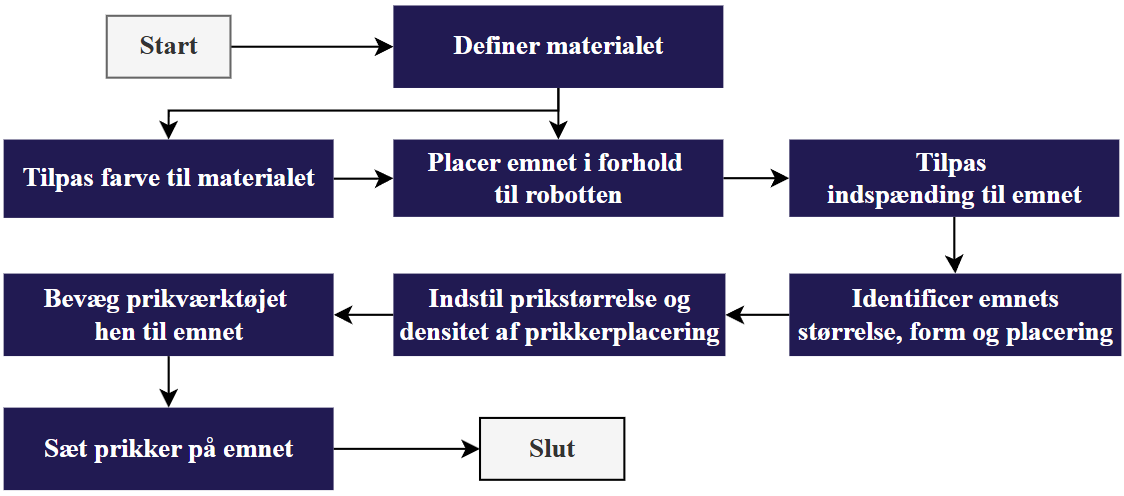
\includegraphics[width=1\linewidth]{Sections/5 Konceptgenerering/Media/Flowchart.png}
    \caption{Flowchart for en robot der skal påsætte speckle patterns}
    \label{fig: flowchart}
\end{figure} \plainbreak{-0.5}

Flowchartet i figur \ref{fig: flowchart} benyttes til at identificere de funktioner og delfunktioner, der ses i figur \ref{Figur: Funktionstræ}. Det er valgt, at opstille alle funktioner i et funktionstræ, for at danne et klart overblik over funktioner og delfunktioner en robot, der sætter speckle patterns skal udføre. Disse benyttes efterfølgende i en morfologisk analyse.  


\newpage
\begin{figure}[H]
\centering
\begin{tikzpicture}
[
    graybox/.style={rectangle, fill=lightgray!20, 
        minimum width=6cm, minimum height=0.8cm, align=center},
    box/.style={rectangle, fill=aaublue, text=white, 
        minimum width=6cm, minimum height=0.8cm, align=center},
    tallbox/.style={rectangle, fill=aaublue, text=white, 
        minimum width=5.8cm, minimum height=1.8cm, align=center, text width=5.8cm},
    arrow/.style={-Stealth, thick}]

% Problemanalyse
\node[tallbox, rotate = 90] (funktioner) {\Large \textbf{Robot til fremstilling af speckle patterns}};

% Funktioner
\node[box, right=1.cm of funktioner.south east, anchor=north west] (bevaegelse) {\textbf{Bevægelse}};
\node[box, below=.8cm of bevaegelse] (kontrolsystem) {\textbf{Kontrolsystem}};
\node[box, below=.8cm of kontrolsystem] (saette) {\textbf{Sætte prikker}};
\node[box, below=.8cm of saette] (fastholde) {\textbf{Fastholde emne}};


%beskrivele Funktion
\node[graybox, above=.2cm of bevaegelse](Funktion){\textbf{Funktioner}};
\draw[lightgray!40, very thick] (1.8,3.1) rectangle (8,-3.2);

%beskrivele delfunktion
\node[graybox, right=1.cm of Funktion](Delfunktion){\textbf{Delfunktioner}};
\draw[lightgray!40, very thick] (8.8,3.1) rectangle (15,-3.2);


% Delfunktioner til Kontrolsystem
\node[box, below=1.3cm of Delfunktion] (brugerflade) {\textbf{Brugerflade}};
\node[box, below=.2cm of brugerflade] (formanalyse) {\textbf{Kalibrering af emne placering}};

% Delfunktioner til Fastholdelse
\node[box, below=1.4cm of formanalyse] (indspaend) {\textbf{Indspænding}};
\node[box, below=.2cm of indspaend] (understot) {\textbf{Understøttelse}};


% Pile
\draw[arrow] (funktioner.south) -- ++(0.5,0) |- (bevaegelse);
\draw[arrow] (funktioner.south) -- ++(0.5,0) |- (saette);
\draw[arrow] (funktioner.south) -- ++(0.5,0) |- (kontrolsystem);
\draw[arrow] (funktioner.south) -- ++(0.5,0) |- (fastholde);

\draw[arrow] (kontrolsystem.east) -- ++(0.5,0) |- (brugerflade);
\draw[arrow] (kontrolsystem.east) -- ++(0.5,0) |- (formanalyse);

\draw[arrow] (fastholde.east) -- ++(0.5,0) |- (indspaend);
\draw[arrow] (fastholde.east) -- ++(0.5,0) |- (understot);

\end{tikzpicture}
\caption{Funktionstræ}
\label{Figur: Funktionstræ}
\end{figure} \plainbreak{-0.5}

Det er valgt ikke at medtage 'tilpas farve til materialet' da der er afgrænset fra farvemidlet i afsnit \ref{Afgrænsning}.


\subsubsection{Bevægelse} \plainbreak{-0.5}
Metode til at flytte prikværktøjet og/eller emnet i forhold til hinanden, der muliggør fremstillingen af et speckle pattern på et 2D plan.



\subsubsection{Kontrolsystem}\plainbreak{-0.5}
%Kontrolsystemet bestemmer hvor og hvornår der skal sættes prikker, og giver feedback til brugeren. Dette er nødvendigt for, at robotten kan påsætte det ønskede speckle pattern, samt give brugeren mulighed for at kunne starte og stoppe maskinen. Kontrolsystemet har to delfunktioner; brugerflade, som skal modtage input og give feedback tilbage til brugeren der betjener robotten og Kalibrering af emnets placering. Kalibreringen er til for, at robotten ved hvor emnet er placeret, dets størrelse og form. For at undgå påsætning af speckle patterns udenfor emnet, er det nødvendig med identifikation af emnets dimensioner.

Det er i afsnit \ref{Afgrænsning} valgt, at afgrænse fra elektronik og software, hvorfor kontrolsystemet ikke medtages i den morfologiske analyse. Det fysiske design af kontrolsystemet har betydning for designet af de mekaniske dele, hvorfor delkoncepter til kontrolsystemet er overfladisk undersøgt i bilag \ref{Bilag - morf til kontrolsystem}.



\subsubsection{Sætte prikker} \plainbreak{-0.5}
En essentiel del af robottens funktion er, at den sætter speckle patterns. Delfunktioner til at sætte prikker vurderes at være så afhængige at hvilken overordnet metode til at sætte prikker der bliver, og kan derfor ikke yderligere specificeres, før den overornede metode er valgt. Dette er fordi løsningerne fra problemanalysens afsnit \ref{DIC afsnit}, har stor variation i metoden til at påsætte prikker og de delfunktioner de kræver. 



\subsubsection{Fastholde emnet} \plainbreak{-0.5}
Emnet skal fastholdes, så emnet ikke flyttes under påsætning af speckle pattern. Fastholdelsen er opdelt i indspænding og understøtning. Emnet må maksimalt flyttes \(\SI{0,01}{mm}\) under påføring af speckle patterns, hvilket nødvendiggør indspænding af emnet, så der ikke sker flytning. Understøtningen defineres som den overflade emnet kan placeres på, hvorefter det kan fastgøres af indspændingen. Understøtningen har til formål at understøtte emnet fra kræfter som tyngdekraften, for at indspændingen kan være så simpel som muligt. 


%Delfunktionerne til kontrolsystem vurderes at være af minimal betydning for vægtningen af konceptforslagene og afhænger af hvilke mekaniske koncepter der vælges. Der laves derfor først en morfologisk analyse af de mekaniske dele, der omfatter; bevægelse, priksætning, indspænding og understøttelse, efterfulgt af en morfologisk analyse af kontrolsystemet.   

 

\plainbreak{2}
\section{Morfologisk analyse af mekaniske dele} \label{Morfologisk analyse - mekaniske dele}
Alle delfunktioner, der omhandler mekaniske dele beskrevet i afsnit \ref{Funktioner}, opsættes i en morfologisk analyse, hvor delløsninger til hver enkelt delfunktion benyttes til at danne samlede løsningskoncepter. Koncepterne skal overholde alle de ufravigelige krav opsat i afsnit \ref{Endelige kravspecifikationer}, for at blive medtaget i den morfologiske analyse.

Antallet af kombinationer af delløsninger, er vurderet for stor til at alle koncepter har kunne gennemgås. Der er fravalgt delløsninger, på baggrund af mangel på effektivitet og nøjagtighed. Der er udvalgt ni koncepter der arbejdes videre med, disse koncepter kan ses i tabel \ref{tab: morfologisk analyse af mekanikse}. Konceptforslagene fra den morfologiske analyse, kan findes ved at følge de forskellige farver/former, der hver repræsenterer et koncept skabt af delkoncepter.


%en farve/form hvert element i det bestemte koncept. Ved at følge for eksempel den lilla cirkel ($\lillacirc$), findes alle delkoncepterne som koncept 1 består af.

%Antallet af kombinationer af delløsninger, har resulteret i en mængde af koncepter vurderet for stor til at alle koncepter har kunne gennemgås

\begin{table}[H]
   \caption{Morfologisk analyse. 1 $=$ \protect\lillacirc, 2 $=$ \protect\bluebox, 3 $=$ \protect\cyanbox, 4 $=$ \protect\blueangle, 5 $=$ \protect\greenangle, 6 $=$ \protect\gulangle, 7 $=$ \protect\orangeangle, 8 $=$ \protect\pinkstar og 9 $=$ \protect\redkant}
    \centering
    \begin{tabular}{|l|p{3.1cm}|p{3.1cm}|p{3.1cm}|p{3.1cm}|} \cline{2-5}      
           \multicolumn{1}{l|}{} & \multicolumn{4}{|c|}{\cellcolor{aaublue} \textcolor{white}{\textbf{Delkoncepter til mekaniske delfunktioner }}} \\ \cline{2-5} \multicolumn{1}{l|}{}  & \multicolumn{1}{c|}{ \cellcolor{lightgray!20} \textbf{1}} & \multicolumn{1}{|c|}{\cellcolor{lightgray!20} \textbf{2}} & \multicolumn{1}{c|}{\cellcolor{lightgray!20} \textbf{3}} & \multicolumn{1}{c|}{\cellcolor{lightgray!20} \textbf{4}}  \\ \cline{2-5} \specialrule{0pt}{0.5pt}{0pt}
          
        %Bevægelse
        \rotatebox[origin=c]{90}{\cellcolor{aaublue} \textcolor{white}{\textbf{Bevægelse }}} & \makecell{\small Lineær bevægelse  \\ \includegraphics[width=0.98\linewidth]{Sections/5 Konceptgenerering/Media/lineær.png} \\ \lillacirc \ \bluebox \ \orangeangle \ \redkant} & \makecell{\small Robotarm \\ 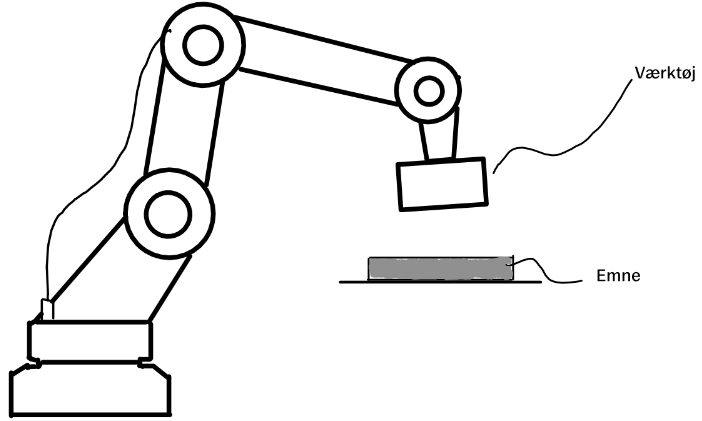
\includegraphics[width=0.98\linewidth]{Sections/5 Konceptgenerering/Media/arm.png} \\ \gulangle} & \makecell{\small Deltarobot\\ 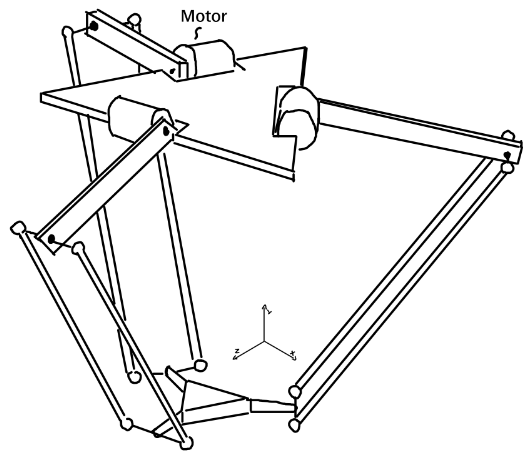
\includegraphics[width=0.98\linewidth]{Sections/5 Konceptgenerering/Media/delta.png} \\ \cyanbox \ \blueangle \ \pinkstar } & \makecell{\small Drejeskive \\ 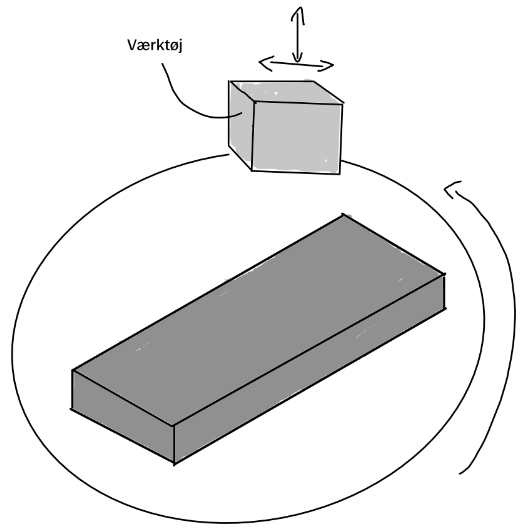
\includegraphics[width=0.98\linewidth]{Sections/5 Konceptgenerering/Media/Drejeskive.png} \\ \greenangle}\\  \specialrule{1pt}{0pt}{0pt}


        %Sæt prik
        \rotatebox[origin=c]{90}{\cellcolor{aaublue} \textcolor{white}{\textbf{\small Sætte prikker}}} & \makecell{\small Sætte dråbe \\ \includegraphics[width=0.8\linewidth]{Sections/5 Konceptgenerering/Media/åbnelukke.png} \\ \lillacirc \ \bluebox \ \cyanbox \ \blueangle \ \greenangle }& \makecell{ \small Spids røre  \\ emnet \\ \includegraphics[width=0.2\linewidth]{Sections/5 Konceptgenerering/Media/spids røre.png} \\ \gulangle \ \orangeangle \ \pinkstar \ \redkant} & \makecell{\small Spray \\ 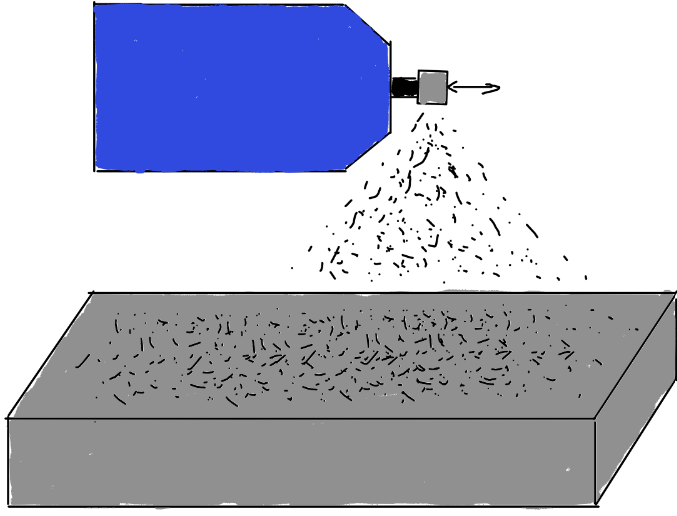
\includegraphics[width=0.8\linewidth]{Sections/5 Konceptgenerering/Media/spray.png}} & \makecell{\small Stempel \\ 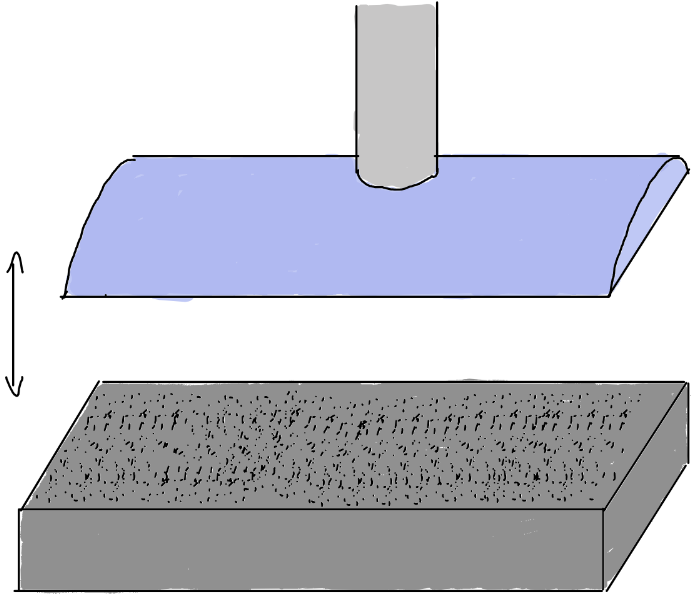
\includegraphics[width=0.98\linewidth]{Sections/5 Konceptgenerering/Media/stempel.png}}  \\ \specialrule{1pt}{0pt}{0pt}

        %Indspænding
        \rotatebox[origin=c]{90}{\cellcolor{aaublue} \textcolor{white}{\textbf{Indspænding}}} & \makecell{\small Press på emnet \\ \includegraphics[width=0.7\linewidth]{Sections/5 Konceptgenerering/Media/Press på emnet.png} \\ \bluebox \ \orangeangle \ \gulangle}  & \makecell{Sug \\ 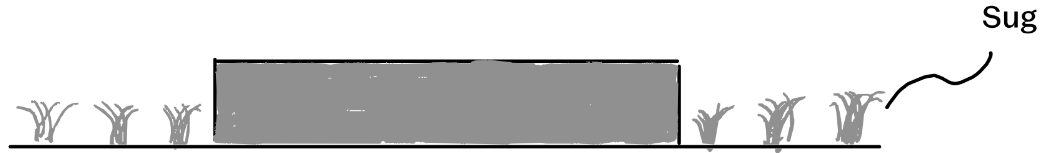
\includegraphics[width=0.98\linewidth]{Sections/5 Konceptgenerering/Media/sug.png} \\ \lillacirc \ \redkant} & \makecell{\small Vakuumpose\\ med fyld \\ 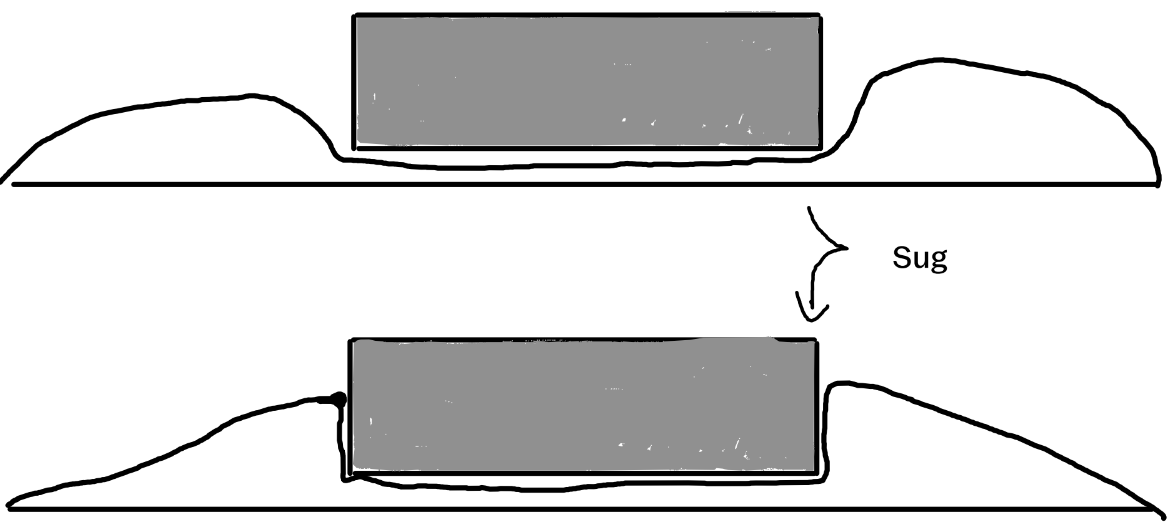
\includegraphics[width=0.98\linewidth]{Sections/5 Konceptgenerering/Media/vakuum.png} \\ \cyanbox \ \greenangle \ \pinkstar}&  \makecell{\small Ru overflade \\ 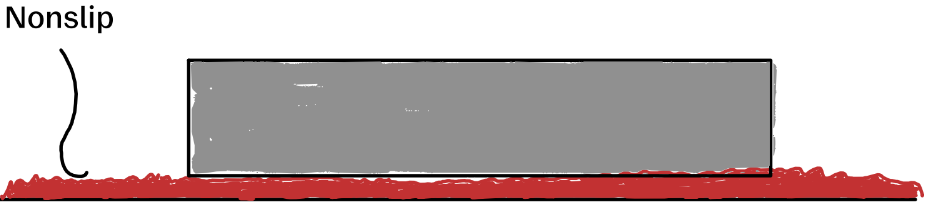
\includegraphics[width=0.98\linewidth]{Sections/5 Konceptgenerering/Media/rug.png} \\ \blueangle}  \\ \specialrule{1pt}{0pt}{0pt}

        %Understøttelse
        \rotatebox[origin=c]{90}{\cellcolor{aaublue} \textcolor{white}{\textbf{Understøttelse}}} & \makecell{\small Plade \\ under emnet \\ \includegraphics[width=0.98\linewidth]{Sections/5 Konceptgenerering/Media/Understøttelse plade.png} \\ \lillacirc \ \cyanbox \ \blueangle \ \greenangle \\ \orangeangle  \gulangle \ \pinkstar \  \redkant } & \makecell{\small Understøttet \\ i punkter \\ \includegraphics[width=0.9\linewidth]{Sections/5 Konceptgenerering/Media/Understøttelse i punkter.png} \\ \bluebox} & &    \\ \hline
        
    \end{tabular}
    \label{tab: morfologisk analyse af mekanikse}
\end{table} \plainbreak{-0.5}

I denne morfologiske analyse, er der set bort fra delløsninger med spray og stempel, se tabel \ref{tab: morfologisk analyse af mekanikse}. Dette er gjort, da der ikke kan findes koncepter med disse delløsninger, som kan skille sig ud og konkurrere på de vilkår der ønskes. Spraymetoden opnår ikke den pålidelighed i prikpræcision, der ønskes for produktet, hvilket er et essentielt punkt, for at produktet vil være konkurrencedygtigt på markedet. Stemplet kan opnå en tilstræklig præcision, i stedet vil det ikke være en tilstrækkelig fordel, da det ikke er nødvendigt med en maskine til at stemple en overflade. Da det er et krav, at der skal laves en robot, giver det ikke mening, at gå videre med den delløsning. Robotarmen og drejeskiven anvendes få gange da det vurderes at deres kompleksitet ikke opvejes med markante fordele. De bliver alligevel inkluderet i et par koncepter, for ikke at gå klip af eventuelle gode løsninger.

Indspændingsdelløsningerne kan også sætte krav til understøtningen. Et eksempel er, at det ikke er muligt at lave sug-funktionen eller vakuumposen med fyld, med en understøttelse i punkter. Dette har medført, at en større andel af koncepterne gør brug af understøtning i form af en plade, frem for understøttelse i punkter. 





\subsection{Konceptforslag til mekaniske dele} \label{Konceptforlag - mekaniske dele}

\begin{figure}[H]
    \centering
    \begin{subfigure}[b]{0.34\textwidth}
        %centering
        \includegraphics[width=\textwidth]
        {Sections/5 Konceptgenerering/Media/1.Løsning.png}
        \caption{Konceptforslag 1 \protect\lillacirc}
        \label{fig:Konceptforslag 1}
    \end{subfigure}
    \begin{subfigure}[b]{0.32\textwidth}
        %centering
        \includegraphics[width=\textwidth]
        {Sections/5 Konceptgenerering/Media/2.Løsning.png}
        \caption{Konceptforslag 2 \protect\bluebox}
        \label{fig:Konceptforslag 2}
    \end{subfigure}
    \begin{subfigure}[b]{0.24\textwidth}
        %centering
        \includegraphics[width=\textwidth]
        {Sections/5 Konceptgenerering/Media/3.Løsning.png}
        \caption{Konceptforslag 3 \protect\cyanbox}
        \label{fig:Konceptforslag 3}
    \end{subfigure}
    \caption{Konceptforslag 1 til 3}
\end{figure} \plainbreak{-0.5}

\textbf{Konceptforslag 1  \protect\lillacirc}  bevæger sig lineært i tre dimensioner og benytter sig af en mekanisme der afsætter dråber, som tager udgangspunkt i en inkjet. Til at fastholde emnet, som skal prikkes, fastspændes det ved brug af sug. Her vil der skabes undertryk under emnet, som vil resultere i at emnet er fastspændt. Sammen med sug vil emnet understøttes af en fast plade under emnet.

\textbf{Konceptforslag 2 \protect\bluebox} 
bevæger sig på samme måde som koncept 1. Koncept 2 bruger som koncept 1 også dråbemekanismen. Denne iteration er unik i fastholdelsen, hvor der bruges pres på emnet fra siderne af, til at holde emnet fast. Her er, fremfor understøttelse i en plade, understøttelse i punkter, som er hvor emnet skal stabiliseres over flere kontaktpunkter.


\textbf{Konceptforslag 3 \protect\cyanbox} 
har sin bevægelse igennem en deltarobot, som trækker i sine arme for at flytte på hovedet over prikfladen. Der gøres også brug af mekanisme der afsætter dråber. Indspændingen laves ved at have en vakuumpose der er fyldt med små kugler, som bliver låst i position efter luften tages ud af posen. Hvis prikobjektet placeres på posen, vil de små kugler position låse objektets position. Dette koncept gør brug af pladen under emnet, som understøtning.

\begin{figure}[H]
    \centering
    \begin{subfigure}[b]{0.27\textwidth}
        %centering
        \includegraphics[width=\textwidth]
        {Sections/5 Konceptgenerering/Media/4.Løsning.png}
        \caption{Konceptforslag 4 \protect\blueangle}
        \label{fig:Konceptforslag 4}
    \end{subfigure}
    \begin{subfigure}[b]{0.28\textwidth}
        %centering
        \includegraphics[width=\textwidth]
        {Sections/5 Konceptgenerering/Media/5.Løsning.png}
        \caption{Konceptforslag 5 \protect\greenangle}
        \label{fig:Konceptforslag 5}
    \end{subfigure}
    \begin{subfigure}[b]{0.35\textwidth}
        %centering
        \includegraphics[width=\textwidth]
        {Sections/5 Konceptgenerering/Media/6.Løsning.png}
        \caption{Konceptforslag 6 \protect\gulangle}
        \label{fig:Konceptforslag 6}
    \end{subfigure}
    \caption{Konceptforslag 4 til 6}
\end{figure} \plainbreak{-0.5}

\textbf{Konceptforslag 4 \protect\blueangle} 
bevæger sig med udgangspunkt i en deltarobot, ligesom koncept 3. Koncept 4 gør brug af mekanismen der sætter dråber. Emnet vil ligge på en rug overflade, så emnet ikke bevæger sig. Derudover vil emnet blive understøttet af en plade under emnet.


\textbf{Konceptforslag 5 \protect\greenangle} 
placerer emnet på en drejeskive, så prikværktøjet kun skal bevæge sig fra side til side (x-retningen), op og ned (z-aksen) og rotere emnet om z-aksen. Prikværktøjet benytter mekanismen der afsætter dråber prikplacering. Emnet indspændes igennem posen med kugler, der sættes i vakuum og låser emnet. Emnet er understøttet af en plade.


\textbf{Konceptforslag 6 \protect\gulangle} 
bruger en flerleddet robotarm til sine bevægelser, som gør rotationer i led til en kontrolleret bevægelse til prikplacering. I dette koncept gøres der brug af tuschmetoden, som indebærer at føre et farvefyldt emne ned og berøre prikfladen, for at overføre farven. Konceptet gør brug af indspænding fra siden, og gør også brug af en plade under emnet til understøtning.

\begin{figure}[H]
    \centering
    \begin{subfigure}[b]{0.3\textwidth}
        %centering
        \includegraphics[width=\textwidth]
        {Sections/5 Konceptgenerering/Media/7.Løsning.png}
        \caption{Konceptforslag 7 \protect\orangeangle}
        \label{fig:Konceptforslag 7}
    \end{subfigure}
    \begin{subfigure}[b]{0.3\textwidth}
        %centering
        \includegraphics[width=\textwidth]
        {Sections/5 Konceptgenerering/Media/8.Løsning.png}
        \caption{Konceptforslag 8 \protect\pinkstar}
        \label{fig:Konceptforslag 8}
    \end{subfigure}
    \begin{subfigure}[b]{0.3\textwidth}
        %centering
        \includegraphics[width=\textwidth]
        {Sections/5 Konceptgenerering/Media/9.Løsning.png}
        \caption{Konceptforslag 9 \protect\redkant}
        \label{fig:Konceptforslag 9}
    \end{subfigure}
    \caption{Konceptforslag 7 til 9}
\end{figure} \plainbreak{-0.5}

\textbf{Konceptforslag 7 \protect\orangeangle} 
benytter en lineær bevægelse til bevægelse af prikværktøjet. Prikmetoden er som koncept 6 tuschmetoden. Der gøres her brug af en indspænding fra siderne. Der bruges en plade under emnet til at understøtte emnet.


\textbf{Konceptforslag 8 \protect\pinkstar}
bevæger sig i form af en deltarobots armjustering. Konceptet skal sætte prikker med tuschmetoden som koncept 6 og 7. Indspændingen kommer af vakuumpose med fyld, der låser emnets placering. Der bruges også her en plade under emnet til understøttelse.


\textbf{Konceptforslag 9 \protect\redkant} 
bevæger sig lineært i tre retninger for at justere prikværktøjet, samt benytter en prik metode, som en tusch. Emnet indspændes ved at danne et undertryk under emnet ved brug af sug, samt bliver understøttet af en plade under emnet.


 
\plainbreak{2}
\subsection{Koncept screening af mekaniske dele} \label{Mekanisk system - vurdering}
%- Tush er mere præcis i prikstørrelse end åbne/lukke \\
%- Delta robot hurtigere end lineær bevægelse \\
For at finde frem til et endeligt løsningskoncept for de mekaniske dele, vurderes de ni udvalgte koncepter igennem en screening. De udvalgte koncepter vurderes ud for et sæt af kriterier, som kan ses i tabel \ref{tab:selektionsskema mekanisk}. Alle delløsninger, som koncepterne består af, er blevet vurderet i forhold til kriterierne (se bilag \ref{Bilag mekaniske delkonceptervurdering}), hvortil de samlede værdier af et koncepts delløsninger, er lig konceptets samlede vurdering. Vurderingerne er sket ved at sætte koncept 1's (\lillacirc) delløsninger som en standard/reference, og dertil vurdere de andre delløsninger, i forhold til koncept 1. Hvert kriterie er tildelt en vægt, som sikrer vigtigere kriterier har større betydning for udfaldet. Vægtene er fremsat på baggrund af vægtningerne fra kapitel \ref{Trin 1-4}, tabel \ref{tab: trin 1 til 4}, og designspecifikationer fra HoQ i kapitel \ref{Kravspecifikation}.

\renewcommand{\arraystretch}{1.6}
\begin{table}[H]
    \centering
    \footnotesize
    \caption{Screening skema. Værdierne er summen af delkoncepternes vurdering som ses i bilag \ref{Bilag mekaniske delkonceptervurdering}.}
    \begin{tabular}{|l|c||c c c c c c c c||r|} \cline{2-10}

        \multicolumn{1}{c}{}& \multicolumn{9}{|c|}{\cellcolor{aaublue} \textcolor{white}{\textbf{Konceptforslag til mekaniske dele}}} \\ \hline
         
        \multicolumn{1}{|c}{\cellcolor{lightgray!20}\textbf{Vurderingskriterier}} & \multicolumn{1}{|c||}{\cellcolor{lightgray!20}\textbf{1 \protect\lillacirc}}  &\multicolumn{1}{c}{\cellcolor{lightgray!20}\textbf{2 \protect\bluebox}} &\multicolumn{1}{c}{\cellcolor{lightgray!20}\textbf{3 \protect\cyanbox}} &\multicolumn{1}{c}{\cellcolor{lightgray!20}\textbf{4 \protect\blueangle}} &\multicolumn{1}{c}{\cellcolor{lightgray!20}\textbf{5 \protect\greenangle}} &\multicolumn{1}{c}{\cellcolor{lightgray!20}\textbf{6 \protect\gulangle}}   &\multicolumn{1}{c}{\cellcolor{lightgray!20}\textbf{7 \protect\orangeangle}} &\multicolumn{1}{c}{\cellcolor{lightgray!20}\textbf{8 \protect\pinkstar}} &\multicolumn{1}{c||}{\cellcolor{lightgray!20}\textbf{9 \protect\redkant}} &\multicolumn{1}{r|}{\cellcolor{lightgray!20}\textbf{Vægt}} \\ \hline
         
    %% Vurdering
        % Præcision af prik størrelse
         \multicolumn{1}{|l|}{\cellcolor{aaublue} \textcolor{white}{\textbf{Præcision af prik størrelse}}} 
         & 0 & 0 & 0 & 0 & 0 & -1 & -1 & -1 & -1 & 3\\ \hline
        % Præcision af prik placering  
         \multicolumn{1}{|l|}{\cellcolor{aaublue} \textcolor{white}{\textbf{Præcision af prik placering}}} 
         & 0 & 0 & -1 & -1 & -1 & 1 & 1 & 0 & 1 & 3 \\ \hline
        % Fastholdelse
         \multicolumn{1}{|l|}{\cellcolor{aaublue} \textcolor{white}{\textbf{Fastholdelse}}} 
         & 0 & 0 & 1 & -3 & 0 & 1 & 1 & 1 & 0 & 5  \\\hline
        % Hurtighed
         \multicolumn{1}{|l|}{\cellcolor{aaublue} \textcolor{white}{\textbf{Hurtighed}}} 
         & 0 & 0 & 0 & 2 & -2 & -2 & -1 & -1 & -1 & 2 \\\hline
        % Brugerinvolvering
         \multicolumn{1}{|l|}{\cellcolor{aaublue} \textcolor{white}{\textbf{Brugerinvolvering}}} 
         & 0 & -2 & 0 & 0 & 0 & -1 & -1 & 0 & 0 & 2 \\\hline
        % Holdbarhed
         \multicolumn{1}{|l|}{\cellcolor{aaublue} \textcolor{white}{\textbf{Holdbarhed}}} 
         & 0 & 1 & 0 & 1 & 0 & -1 & 0 & -1 & -1 & 1 \\\hline
        % Kompleksitet ved fremstilling
         \multicolumn{1}{|l|}{\cellcolor{aaublue} \textcolor{white}{\textbf{Kompleksitet ved fremstilling}}} 
         & 0 & 1 & -1 & 1 & 0 & 1 & 2 & 0 & 1 & 1 \\\hline
        % Kompleksitet ved samling
        \multicolumn{1}{|l|}{\cellcolor{aaublue} \textcolor{white}{\textbf{Kompleksitet ved samling}}} 
        & 0 & -1 & 0 & 1 & 0 & -1 & 0 & 1 & 1 & 1 \\ \hline \specialrule{0pt}{2pt}{0pt} \cline{1-10}
%% Samlet score og rank
         \multicolumn{1}{|r|}{\cellcolor{lightgray!10} \textbf{Vægtet score}}& 0 & -3 & 1 & -11 & -7 & -2 & 3 & 0 & \multicolumn{1}{c|}{-1}  & \multicolumn{1}{c}{} \\\cline{1-10} 

         \multicolumn{1}{|r|}{\cellcolor{lightgray!10}\textbf{Rangering}}& 3 & 7 & \multicolumn{1}{c}{\cellcolor{OliveGreen}\textbf{2}} & 9 & 8 & 6 &  \multicolumn{1}{c}{\cellcolor{OliveGreen}\textbf{1}} & 3 & \multicolumn{1}{c|}{5}  & \multicolumn{1}{c}{} \\\cline{1-10}
    \end{tabular}
    \label{tab:selektionsskema mekanisk}
\end{table} \plainbreak{-0.5}

Ud fra screeningen blev koncept 3 (\cyanbox) og 7 (\orangeangle) vurderet til at være de to bedste kandidater. De to konceptforslags forskellige delløsninger blev sammenlignet, for at undersøge om en kombination, af de to eventuelt kunne skabe et bedre koncept. Det resulterede i, at koncept 7 i kombination med koncept 3's sæt prik delløsning, vil øge præcisionen og derved danne det bedste koncept. Det sammensatte koncept 10 ($\protect\mathcolor{BrickRed}{\clubsuit}$) (bilag \ref{Bilag mekaniske delkonceptervurdering}) får 4 point i den vægtede score, hvilket er 1 point mere end konceptforslag 7. Screeningsskemaet for det endelige koncept kan ses i bilag \ref{Bilag mekaniske delkonceptervurdering}. 



\begin{comment}
\begin{table}[H]
    \caption{}
    \centering
    \begin{tabular}{|c|c|c|c|} 
        \hline
        \multicolumn{4}{|c|}{\cellcolor{aaublue} \textcolor{white}{\textbf{Endelig mekanisk koncept }}} \\ \hline
        \rowcolor{lightgray!10} Bevægelse & Sætte prikker& Indspænding & Understøttelse \\ \hline
        \multicolumn{1}{|p{3.4cm}|}{
        \includegraphics[width=0.80\linewidth]{Sections/5 Konceptgenerering/Media/lineær.png}} &  
        \multicolumn{1}{p{3.4cm}|}{\includegraphics[width=0.80\linewidth]{Sections/5 Konceptgenerering/Media/åbnelukke.png}} &
        \multicolumn{1}{p{3.4cm}|}{\includegraphics[width=0.80\linewidth]{Sections/5 Konceptgenerering/Media/Press på emnet.png}} &
        \multicolumn{1}{p{3.4cm}|}{ \includegraphics[width=0.80\linewidth]{Sections/5 Konceptgenerering/Media/Understøttelse plade.png}} \\ \hline
    \end{tabular}
    \label{tab: endeligkonceptmekanisk}
\end{table}
\end{comment}



\begin{comment}
\begin{table}[H]
    \centering
    \caption{Selektion skema, hvor 0 = neutral, + = bedre end og - = værre end.  Den samlet score er beregnet ved "Sam af +" + "Sum af -"}
    \begin{tabular}{|>{\columncolor{lightgray!20}}c|c|c|*{1}{>{\centering\arraybackslash}p{.4cm}} || *{8}{>{\centering\arraybackslash}p{.4cm}|}} \cline{4-12}

        \multicolumn{3}{c}{}& \multicolumn{9}{|c|}{\cellcolor{aaublue} \textcolor{white}{\textbf{Konceptforslag til mekaniske dele}}} \\ \cline{4-12}
         
        \multicolumn{3}{c}{} & \multicolumn{1}{|c||}{\cellcolor{lightgray!20}\textbf{1}}  &\multicolumn{1}{c|}{\cellcolor{lightgray!20}\textbf{2}} &\multicolumn{1}{c|}{\cellcolor{lightgray!20}\textbf{3}} &\multicolumn{1}{c|}{\cellcolor{lightgray!20}\textbf{4}} &\multicolumn{1}{c|}{\cellcolor{lightgray!20}\textbf{5}} &\multicolumn{1}{c|}{\cellcolor{lightgray!20}\textbf{6}}   &\multicolumn{1}{c|}{\cellcolor{lightgray!20}\textbf{7}} &\multicolumn{1}{c|}{\cellcolor{lightgray!20}\textbf{8}} &\multicolumn{1}{c|}{\cellcolor{lightgray!20}\textbf{9}} \\ \hline
         
    %% Vurdering
        % Præcision af prik størrelse
        & \multicolumn{2}{|l|}{\cellcolor{aaublue} \textcolor{white}{\textbf{Præcision af prik størrelse}}} &o &o &o &o &o &+ &+ & + &+\\ \cline{2-12}
        % Præcision af prik placering  
        & \multicolumn{2}{|l|}{\cellcolor{aaublue} \textcolor{white}{\textbf{Præcision af prik placering}}} &o &o &+ &+ &- &o &o & o & o \\ \cline{2-12}
        % Fastholdelse
        & \multicolumn{2}{|l|}{\cellcolor{aaublue} \textcolor{white}{\textbf{Fastholdelse}}} &o &+ &o &- &o &+ &+ &o &o \\\cline{2-12}
        % Alsidighed
        & \multicolumn{2}{|l|}{\cellcolor{aaublue} \textcolor{white}{\textbf{Hurtighed}}} & & & & & & & & & \\\cline{2-12}
        % Holdbarhed
        & \multicolumn{2}{|l|}{\cellcolor{aaublue} \textcolor{white}{\textbf{Holdbarhed}}} &o &+ &- &+ &- &- &o &o &+  \\\cline{2-12}
        % Kompleksitet ved fremstilling
        & \multicolumn{2}{|l|}{\cellcolor{aaublue} \textcolor{white}{\textbf{Kompleksitet ved fremstilling}}} &o &+ &- &+ &- &- &o &o &+  \\\cline{2-12}
        % Kompleksitet ved samling
        \multirow{-7}{*}{\rotatebox{90}{\textbf{Vurderingskriterier}}} & \multicolumn{2}{|l|}{\cellcolor{aaublue} \textcolor{white}{\textbf{Kompleksitet ved samling}}} & o &o &+ &o &o &o &o &- &o \\ \hline \specialrule{0pt}{2pt}{0pt} \cline{2-12}

%% Summen af værdier
        % Sum af o
        \multicolumn{1}{c}{\cellcolor{white}} & \multicolumn{2}{|r|}{\cellcolor{lightgray!10} \textbf{sum af o}} & 8 & &  & & & & & &  \\\cline{2-12}
        % Sum af +
        \multicolumn{1}{c}{\cellcolor{white}} & \multicolumn{2}{|r|}{\cellcolor{lightgray!10} \textbf{sum af +}} & 0 & &  & & & & & &  \\\cline{2-12}
        % Sum af -
        \multicolumn{1}{c}{\cellcolor{white}} & \multicolumn{2}{|r|}{\cellcolor{lightgray!10} \textbf{sum af -}} & 0 & &  & & & & & &  \\\cline{2-12}  \specialrule{0pt}{2pt}{0pt} \cline{2-12}  

%% Samlet score og rank
         \multicolumn{1}{c}{\cellcolor{white}} & \multicolumn{2}{|r|}{\cellcolor{lightgray!10} \textbf{Samlet score}}& 0 & &  & & & & & &  \\\cline{2-12}

        \multicolumn{1}{c}{} & \multicolumn{2}{|r|}{\cellcolor{lightgray!10}\textbf{Rangering}} & 5 & &  & & & & & &  \\\cline{2-12}
    \end{tabular}
    \label{tab:selektionsskema mekanisk}
\end{table}

  
\end{comment}
 

 


\plainbreak{2}
\section{Koncept} \label{Endelig koncept}
Illustration af det endelige konceptforslag ses i figur \ref{fig: endelig koncept}. Konceptet er konceptforlag 10 ($\protect\mathcolor{BrickRed}{\clubsuit}$) fra afsnit \ref{Mekanisk system - vurdering} med et kamera til kalibrering af emne placering og en touchskærm som brugerflade. Kameraet og touchskærmen er valgt i bilag \ref{Bilag - morf til kontrolsystem}, og tages højde for i den videre udvikling af de mekaniske dele. 

\begin{figure}[H]
    \centering
    \includegraphics[width=0.7\linewidth]{Sections/5 Konceptgenerering/Media/Endelige løsning.png}
    \caption{Koncept 10 $\protect\mathcolor{BrickRed}{\clubsuit}$. }
    \label{fig: endelig koncept}
\end{figure} \plainbreak{-0.5}

Konceptet videreudvikles i følgende del, hvor mekanismen der skal sætte dråber undersøges yderligere og der foretages valg af bevægelsesmekanisme til den lineære bevægelse. Dette sker med udgangspunkt i designspecifikationer og ufravigelige krav fra afsnit \ref{Endelige kravspecifikationer}.


%Det endelige koncept rejser en række tekniske problemstillinger, der kræver nærmere undersøgelse, herunder mekanismen, som er ansvarlig for at afsætte dråber, hvordan denne mekanisme fungerer, og hvordan den skal fungere i forhold til konceptet. Derefter, hvordan man opnår den højeste præcision ved lineær bevægelse, og forskellige måder at presse på emnet er også blandt disse spørgsmål.


%Hvordan specifikt "åbne/lukke" mekanisme skal fungere er nok det største nye spørgsmål. Derefter, hvordan man opnår den højeste præcision ved lineær bevægelse og forskellige måder at presse på emnet.

\begin{comment}
\begin{figure}[H]
    \caption{Billede af det endelige koncept samt tabel over de delfunktioner den består af.}
    \label{fig:Endelige konceptdesign}
    \small
    \begin{tabularx}{\textwidth}{|Y|Y|Y|Y|p{1pt}|Y|Y|} 
        \hline
        \rowcolor{aaublue}\multicolumn{4}{|c}{\textcolor{white}{\textbf{Mekanisksystem}}} & & \multicolumn{2}{c|}{\textcolor{white}{\textbf{Kontrolsystem }}} \\ \hline
        \rowcolor{lightgray!30} Bevægelse & Sætte prikker & Indspænding & Understøttelse & & Brugerflade & Formanalyse \\ \hline
        \includegraphics[width=0.80\linewidth]{Sections/5 Konceptgenerering/Media/lineær.png} & 
        \includegraphics[width=0.80\linewidth]{Sections/5 Konceptgenerering/Media/åbnelukke.png} &
        \includegraphics[width=0.80\linewidth]{Sections/5 Konceptgenerering/Media/Press på emnet.png} &
        \includegraphics[width=0.80\linewidth]{Sections/5 Konceptgenerering/Media/Understøttelse plade.png} & &
        \includegraphics[width=0.80\linewidth]{Sections/5 Konceptgenerering/Media/Computer.png} & 
        \includegraphics[width=0.80\linewidth]{Sections/5 Konceptgenerering/Media/Kamera.png} \\ \hline
        
        \rowcolor{aaublue}\multicolumn{7}{|c|}{\textcolor{white}{\textbf{Endelig koncept}}} \\ \hline
        \multicolumn{7}{|c|}{\includegraphics[width=0.80\linewidth]{Sections/5 Konceptgenerering/Media/Endelige løsning.png}} \\ \hline
    \end{tabularx}
\end{figure}
  
\end{comment}


\plainbreak{2}
\input{Sections/5 Konceptgenerering/5 Løsningsanalyse}
\subsection{Prikdosering} \label{Prikplacering}
Der er i den morfologiske analyse fundet frem til, at prikkerne påføres emnet med en mekanisme der doserer en dråbe. Dette sker uden kontakt til emnet, og der vælges at gøre brug af en eksisterende løsning, der implementeres i robotten. Af eksisterende metoder til præcis dosering af dråber er følgende; Piezoelectric Jet Valves (PeJV), Piezoeletric Pump (PeP) og Thermal InkJet (TIJ) udvalgt. 

%De 3 metoder undersøges, hvorefter en udvælges. 

%Ud fra vurderingen i \ref{Mekanisk system - vurdering} skal der udvikles en løsningen hvor "farven", påføres materialet uden kontakt. Der vil i det følgdene undersøges løsning muligheder, til at opnå prikplacering. Dette vælges som det første, for at lave overslags bergninger på stellets styrke. 


\textbf{Piezoelectric Jet Valves (PeJV)} fungere ved at en piezoelektrisk aktuator, flytter et stempel op og ned. Når stemplet flyttes op, kan væske bevæge sig ind i dyse hovedet. I det stemplet sænkes igen, vil stemplets kontakt med dyse hovedet, gør at væsken skydes ud af dysen, som vist i figur \ref{fig:PeJV}.

\begin{figure}[H]
    \centering
    \includegraphics[width=0.6\linewidth]{Sections/5 Konceptgenerering/Media/PEJV.png}
    \caption{Ilustration af piezoelektrisk aktuator}
    \label{fig:PeJV}
\end{figure} \plainbreak{-.5}

 Processen gentages for hver gang der skal sættes en prik. Brugen af piezoelektrisk aktuator, betyder der er en høj kontrol af stemplets bevægelse, hvilket medfører en høj væske doseringspræcision, helt ned til \(\SI{0,5}{nL}\). Yderligere betyder brugen af piezoelektrisk aktuator, at cyklussen kan udføres med op til \(\SI{3000}{Hz}\). (\cite{VIEWEG2025JetDV-6210}; \cite{Hoath2016FundamentalsDroplets})


\plainbreak{1}
\textbf{Piezoeletric Pump (PeP)} bruger en piezoelektrisk aktuator til at danne et undertryk, som åbner indgangen til et kammer og trækker farve ind i kammeret. Dette fremgår af figur \ref{fig:PeMP}. Når kammeret er fyldt op bruges den piezoelektriske aktuator til at skabe et overtryk, der åbner udgangen og skubber farven ud. Ved PeP skubbes farven ud af et tryk, i modsætning til at blive skudt ud som ved PeJV. Dette resulterer i et simplere system, med et begrænset antal dele der bevæges. (\cite{Benaissa2012PerformancesPiezo-pump}; \cite{Hoath2016FundamentalsDroplets})

\begin{figure}[H]
    \centering
    \includegraphics[width=1\linewidth]{Sections/5 Konceptgenerering/Media/pumpe.png}
    \caption{Illustration af piezoelektrisk pumpe}
    \label{fig:PeMP}
\end{figure} \plainbreak{-0.5}

PeP bruges ofte til at pumpe en væske kontinuerligt, hvilket betyder der ikke er gode muligheder for udføre doseringer, der kræver pauser imellem. Dette betyder for at gøre brug af PeP, skal der gøres brug af en kontinuerligt væskebevægelse, hvortil et andet system skal opsamle væsken der ikke skal doseres. Sådan et system introducerer kompleksitet tilbage i systemet.

\textbf{Thermal InkJet (TIJ)} fungerer ved, at blæk opvarmes indtil det fordamper og der opnås en indre boble i blækket. Den indre boble vil udøve et tryk på blækket, som vil medføre at blækket skubbes ud af en dyse. Når blækket er skubbet tilstrækkeligt ud af dysen, vil boblen kollapse, hvilket resultere i at der skabes et undertryk, der trækker nyt blæk ind til opvarmning, hvorefter processen gentages, dette illustreres på figur \ref{fig:TIJ figur}. 
Ved at gøre brug af opvarmning, har TIJ en begrænsning i forhold til hvor hurtigt der kan printes, da nye bobler først kan dannes efter forrige boble har forladt dysen. \parencite{Hoath2016FundamentalsDroplets}


\begin{figure}[H]
    \centering
    \includegraphics[width=0.35\linewidth]{Sections/6 Detaljeløsning/Media/TIJ figur 2.png}
    \caption{Illustration af thermal injekt teknik.}
    \label{fig:TIJ figur}
\end{figure} \plainbreak{-.5}

\subsubsection{Valg af doserings metode}  \plainbreak{-.5}
Det vælges at der anvendes en PeJV, fordi den kombinerer høj nøjagtighed, med høj gentagelseshastighed (op imod flere tusinde dråber i sekundet) uden at belaste farvestoffet med varme, hvilket sikre ensartede prikker i den ønskede størrelse. Samtidigt kræver PeJV ikke konstant flow og opsamling af overskydende væske, og den kan producere prikker i et bredt spænd. Alle disse egenskaber understøtter direkte de fremsatte krav omkring nøjagtighed, hastighed og fleksibilitet i løsningen. 

\plainbreak{2}
\subsection{Lineær bevægelse} \label{løsningsanal: Lineær bevægelse}
Det ønskes at finde en optimal bevægelsesform til flytning af prikemnet under prikpåføring. Fra designspecifikationer kan det ses, at der lægges vægt på præcision og hastighed af prikplacering. Dette vil bruges til at vægte forskellige lineære løsningsforslag, og vurdere den bedste løsning.
Af disse grunde, vælges der at udelukke løsninger der er upræcise, langsomme og evt. for komplicerede til at være en optimal løsning, dette efterlader valget mellem et tandremdrevet og et skruedrevet system. \parencite{IndustrialQuickSearch2025LinearPrinciples}

\textbf{Skruedrevet system} omfatter de to mest udbredte metoder; kugleskruer og ledeskruer. Ledeskruer omdanner roterende bevægelse til lineær bevægelse, gennem et gevind på skruen, hvortil genstanden der skal flyttes sidder på skruen se figur \ref{fig:Ledeskrue - skitse}. Ved at bevæge gevindet vil genstanden bevæge sig med gevindets spiral og derved bevæge sig frem ad.

Ledeskruer kræver færre dele og mindre vedligeholdelse end en kugleskrue. Tilgengæld er den mindre effektiv, grundet en større kontaktflade. Generelt gør ledeskruers simplere design, som ses i figur \ref{fig:Ledeskrue - skitse}, den billigere, men en kugleskrue kan have højere nøjagtighed og flytte tungere laster. Kugleskruers primære fordel er den lavere friktion og dermed højere effektivitet. Her er effektivitet et udtryk for forholdet mellem overført kraft og energi tabt til varme. (\cite{UniversalThreadGrindingCompany2020PrecisionAssemblies}; \cite{IndustrialQuickSearch2025LeadBenefits})

\begin{figure}[H]
    \centering
    \begin{subfigure}[b]{0.49\textwidth}
    \centering
        \includegraphics[width=\linewidth]{Sections/5 Konceptgenerering/Media/Ledeskrue-skitse.png}
      \caption{Skitse af ledeskrue}
       \label{fig:Ledeskrue - skitse} % Viljams mor når mig når(s)
  \end{subfigure}
    \hfill
  \begin{subfigure}[b]{0.49\textwidth}
    \centering
    \includegraphics[width=\linewidth]{Sections/6 Detaljeløsning/Media/Ball nut.png}
    \caption{Kugleskrue illustration}
    \label{fig: Balls nut} % Mig når mig når når mig når viljams mor
  \end{subfigure}
    \caption{}
\end{figure} \plainbreak{-0.5}

Kugleskruer omsætter rotations kraft til lineære kraft, denne transformation opnås ved at rotere en skrue, hvorpå en kuglemøtrik er monteret. Kuglemøtriken indholder en mængde kugler, som bevæger sig i skurens gevind. Kuglernes bevægelse i gevindet resultere i at kuglemøtriken skubbes langs skruen. Kuglemøtrikens udformning muliggøre at kuglerne kan genanvendes, ved at når de når enden føres de gennem kuglemøtriken tilbage til fronten af kuglerækken (Se figur \ref{fig: Balls nut}). Kugleskruer har en højere effektivitet end ledeskruer, da rullende kugler har en lavere friktions koeficient end to flader, der gnider mod hinanden, som i en ledeskrue. Kugleskruers afvigelse ligger lidt under $\SI{0,0001}{mm}$. (\cite{Jaffe2025PrecisionGround}; \cite{IndustrialQuickSearch2025BallBenefits})


\textbf{Tandremsdrevede systemer} er kendetegnet ved, at en motor roterer en tandremskive hvorpå tandremmer sidder. Denne tandrem er koblet til en genstand, der ønskes at bevæges langs bæltets længde. Når tandremmen roteres den ene vej, vil emnet blive trukket i den retning, og modsatte retning hvis rotationsvejen vendes. Det tandremsdrevede system, er effektivt under lange arbejdslængder, og kan opnå store hastigheder. Tandremmene har en risiko for at glide, samt består af mere elastiske materialer end skruerne, hvilket kan medføre en afvigelse i præcision. Tandremmes afvigelse ligger omkring \(\SI{0,001}{mm/mm}\) \parencite{Rollco2022BallWhat}. 

\begin{figure}[H]
    \centering
\includegraphics[width=0.6\linewidth]{Sections/5 Konceptgenerering/Media/Illustration af tandrem 7.png}
    \caption{Illustration af tandrem.}
    \label{fig: Illustration af tandrem}
\end{figure} \plainbreak{-.5}

Grundet materialerne tandremmen er lavet af varierer, sammen med remmene bliver svage i løbet af deres levetid, betyder dette at præcisionen af tandremme afhænger af mange faktorer. For at tandremssystemer kan opnå den nødvendige præcision, kræver det mere justering og er mindre pålideligt over løsningens levetid. \parencite{Casillo2025Belt-DrivenInc} 


\subsubsection{Valg af lineær bevægelse}  \plainbreak{-0.5}
Af forrige fremlagte muligheder, er kun ledeskruer og kugleskruer interessante, da der her skal fokuseres på korte afstande og stor præcision. Lede- og kugleskruer ligger begge mere end 1/5 under den maksimal acceptabel afvigelse på \(\SI{\pm0,1}{mm}\) over \(\SI{200}{mm}\), som er den største værdi i arbejdsområdets grænseværdi, hvilket gør begge brugbare.

Under prikplacering vil der ske mange accelerationer før arbejdsområdet er udfyldt, når der skiftes retninger. Dette betyder at en større acceleration vil gøre prikprocessen kortere. Accelerationen er en konsekvens af effektiviteten af skruen. Ledeskruer har typisk mellem 50\% og 70\% effektivitet, hvorimod kugleskuer har typisk over 90\% effektivitet. \parencite{johoty.com2025BallBest}

En ledeskrue bliver valgt til den lineære bevægelse, på trods af en lavere mekanisk effektivitet sammenlignet med en kugleskrue. Ledeskruer leverer den nødvendige præcision ($\approx \SI{d-4}{mm/mm}$) over kortere længder, og samtidigt kræver færre komponenter og minimal vedligeholdelse i forhold til kugleskruer. Deres simple design betyder også lavere materialeforbrug, samt færre dele at udskifte i tilfælde af nedbrud. 
\plainbreak{2}
\subsection{Endeligt koncept} \label{Endeligt koncept}
Det endelige konceptdesign fremgår af figur \ref{fig:skitse af endeligt koncept med navne}, hvor tre sæt af ledeskruer og følgestænger, danner bevægelsessystemet i henholdsvist to x-akser og én y akse.

\begin{figure}[H]
    \centering
    \includegraphics[width=0.7\linewidth]{Sections/6 Detaljeløsning/Media/Skitse med navne.png}
    \caption{Skitse af endeligt koncept med navne}
    \label{fig:skitse af endeligt koncept med navne}
\end{figure} \plainbreak{-.5}

Opsætningen er valgt med fokus på at sikre præcis lineær bevægelse af PeJV'en hen over emnet. I figuren ses, hvordan hovedet bevæger sig langs to parallelle følgestænger, hvor ledeskruen står for fremdriften. Denne mekaniske opsætning gør systemet stabilt, hvilket er nødvendigt for at opnå den påkrævede præcision.




\chapter{Problemanalyse} \label{Problemanalyse}
Det følgende afsnit har til formål at afdække anvendelse og fremstilling af speckle patterns til brug ved DIC, herunder undersøgelse af hvilke parametre, der beskriver et optimalt speckle pattern. Derefter defineres og undersøges robotter for at opnå den nødvendige forståelse for deres mekanismer, så en løsning til fremstilling af speckle patterns kan udvikles.

% --- DIC ---
\section{Digital Image Correlation} \label{DIC afsnit}
DIC er en optisk metode, der anvender digitale billeder til at måle deformation, bevægelse og tøjning i materialer. DIC fungerer ved at sammenligne billeder taget før, under og efter deformation for at måle forskydninger og udregne tøjninger. Metoden gør det muligt at undersøge deformationer over hele emnet og omkring revner. (\cite{Zaya2023ApplicationReview})

\begin{figure}[H]
    \centering
    \includegraphics[width=0.85\linewidth]{Sections/2 Problemanalyse/Media/Speckle pattern subset matrix.png}
    \caption{Illustration af speckles pattern, i øverste højre hjørne ses et subset på $20 \times 20 \text{pixels}$ . Det er genereret med software fra Correlated Solutions (\cite{CorrelatedSolutions2025SpeckleInc.})}
    \label{fig:speckle pattern subset}
\end{figure} \plainbreak{-0.5}

DIC starter med et reference billede taget før deformation, eventuelt efterfulgt af billeder taget under deformationsprocessen, samt et billedet efter deformation. Computersoftware bruger forskellen mellem referencebilledet og de efterfølgende billeder, til at finde deformationer, som herefter udregnes til tøjninger i prøven. Softwaren gør dette ved at identificere subsets af pixels (se figur \ref{fig:speckle pattern subset}) i reference billedet, og derefter finder samme deformerede subset på billedet hvor emnet er deformeret. (\cite{Zaya2023ApplicationReview})

DIC benyttes både til undersøgelser af plane emner (2D), samt rumlige emner (3D). I 2D undersøgelser må materialet ikke deformere sig ud af planet, da denne bevægelse ikke kan blive set af kameraet. 3D DIC benytter sig af to eller flere kameraer, og er optimal i situationer, hvor et materiale bevæger sig fra planet til rummet (figur \ref{fig:2D og 3D DIC}).

\begin{figure}[H]
    \centering
    \includegraphics[width=0.9\linewidth]{Sections/2 Problemanalyse/Media/DIC 2D eller 3D.png}
    \caption{Opstilling af 2D og 3D digital image correlation (\cite{Wang2023FiberMonitoring})}
    \label{fig:2D og 3D DIC}
\end{figure} \plainbreak{-0.5}

Opstillingen med flere kameraer giver mulighed for, at tage flere billeder fra forskellige vinkler, og ved hjælp af stereo triangulering, danne en 3D model af objektet. (\cite{Byrne2020DigitalSoftware})


Speckle patterns opdeles i denne rapport i to dele, mikro- og makroskala. I denne rapport defineres mikroskala som den størrelse, der ikke kan opfanges med det blotte øje, og makroskala er den størrelse, der kan fanges med det blotte øje. Der vælges at arbejde i makroskala, med prikker ned til \SI{0,1}{mm} i diameter, fordi det vurderes, at være realistisk at lave speckle patterns i en størrelsesorden man kan se, og ikke mindre.


%Vinklen mellem to kameraer og objektet kaldes stereo vinklen. Denne vinkel kan justeres afhængig af ønsket resultat. Hvis man ønsker større undersøgelse rettet mod et plan, kan vinklen mindskes, og til en rumlig undersøgelse med bevægelse ud af planet, kan vinklen øges. Den optimale vinkel for 3D DIC er mellem 15\degree og 35\degree. (\cite{Bigger2018ACorrelation}) 



\subsection{Alternative målemetoder}
Alternativerne til DIC er primært strain gauges og ekstensometre. Generelt kan de betegnes som spotmålere, det vil sige de måler over et begrænset område, tilgengæld giver de mere nøjagtige målinger end DIC.

\begin{figure}[H]
    \centering
    \begin{subfigure}{0.48\textwidth}
        \centering
        \includegraphics[width=0.8\linewidth]{Sections/2 Problemanalyse/Media/strain gauge.png}
        \caption{Lineær strain gauge der ikke er monteret \parencite{IndustrialQuickSearch2025PrinciplesGauges}}
        \label{fig:straingauge}
    \end{subfigure}
    \begin{subfigure}{0.48\textwidth}
        \centering
        \includegraphics[width=0.7\linewidth]{Sections/2 Problemanalyse/Media/ekstensometer.png}
        \caption{Clip-On ekstensometer monteret \parencite{ZwickRoellExtensometers}}
        \label{fig:ekstensometer}
    \end{subfigure}
    \caption{}
    \label{alternativertildic}
\end{figure} \plainbreak{-0.5}

\textbf{Strain gauges} består af en tynd metalstribe, typisk i zigzaggede parallelle linjer (se figur \ref{fig:straingauge}), på et fleksibelt, isolerende materiale med en form for klistrende underside. Tøjningen findes ved måling af ændringen i modstand, jo mere den deformeres jo højere vil modstanden blive. 

\textbf{Ekstensometre} måler ændringen i afstanden mellem dens to arme, se figur \ref{fig:ekstensometer}. Ekstensiometre kommer i flere varianter der afhænger af,  hvordan armene påsættes emnet.


 

%Siden sin begyndelse i slut 1900-tallet, har DIC gennem årene udviklet sig, og blevet benyttet til en række af forskellige materialeundersøgelser og er blevet til en populær eksperimentel metode blandt andet grundet kosteffektivitet. Materialeundersøgelser som DIC har været igennem inkluderer metaller, polymerer, kompositter, samt biologiske materialer. Disse undersøgelser finder sted på både mikro- og makroskopisk skala, fra millimeter til flere meter. Herved har man også fundet materialer, som ikke er egnet til DIC grundet specifikke faktorer. Nogle af disse inkluderer: Gennemsigtige, bløde eller reflekterende materialer. Løsninger på disse lyder på overfladebelægning af gennemsigtig materiale, benytte speckles af matsort på reflekterende overflader. På bløde materialer er det mere besværligt, men et kamera med en høj rate af billeder i sekundet skal anvendes, grundet skrøbelighed og hurtig deformation. (\cite{Dong2017ACorrelation}; \cite{Bigger2018ACorrelation}) 


% --- Speckle patterns --- 
\plainbreak{2} \section{Speckle pattern} \label{Speckle pattern} 
Speckle patterns er betegnelsen for et billede eller område med prikker, der anvendes til måling af deformationer og tøjninger i materialer ved brug af DIC \parencite{Dong2017ACorrelation}. Prikkerne i et speckle pattern er ikke foruddefineret til at have én bestemt størrelse, form, kontrast, densitet og fordeling. Disse parametre afhænger af størrelsen på emnet der undersøges, kameraets opløsning samt påføringsmetoden. Eksempler på forskellige speckle patterns kan ses i figur \ref{fig:speckle pattern}.\\

\begin{figure}[H]
    \centering
    \includegraphics[width=\linewidth]{Sections/2 Problemanalyse/Media/speckle pattern forskellige.png}
    \caption{Eksempler på computergenereret speckle patterns med forskellig densitet og prikstørrelse. Speckle pattern er genereret med software fra Correlated Solutions (\cite{CorrelatedSolutions2025SpeckleInc.})}
    \label{fig:speckle pattern}
\end{figure} \plainbreak{-0.5}

Præcisionen af DIC afhænger blandt andet af det anvendte speckle patterns kvalitet, der kan vurderes ved brug af softwareprogrammer. Programmerne benytter forskellige metoder til kvalitetsvurdering, der vurderer parametre som størrelse, form og fordeling af prikkerne.  
\plainbreak{1} \subsection{Optimale speckle patterns} \label{Optimale speckle patterns}

Et godt speckle pattern er karakteriseret ved høj kontrast mellem prikker og baggrund, og et tilfældigt mønster, der er jævnt fordelt og udgør mellem 50\% og 70\% af billedet. Prikkerne skal have en ensartet radius, samt have en størrelse på mellem $3\times3$ og $5\times5$ pixels. Derudover skal prikkerne være indenfor kameraets field of view (FOV). I denne rapport referer FOV til længden af det område kameraet observerer, det er dermed en konsekvens af dets brændvidde og afstand til emnet. (\cite{Dong2017ACorrelation}; \cite{Su2022Glare:Pattern}; \cite{Gagnon2024ThePatterns}).  


%------
\subsubsection{Høj kontrast}\plainbreak{-0.4} 
DIC benytter gray-level til vurdering af prikkernes placering på overfladen. Gray-level er en grå-skala værdi fra 0\% til 100\%, der beskriver lysintensiteten i et enkelt pixel. Et gray-level på 100\% ses som hvid, hvor 0\% er helt sort, gray-level værdien angiver mængden af lys. Værdierne angives fra 0 til 255 for et 8-bit kamera. Det er nødvendigt med høj kontrast, så kameraet kan opfange forskellen mellem prikker og baggrund. Ofte bruges sorte prikker på hvid baggrund, eller hvide prikker på sort baggrund, idet disse har størst forskel mellem prikkerne og baggrundens gray-level. Forskellen mellem baggrund og prikker skal være på minimum 52 point, for at opnå en optimal værdi, skal denne forskel ligge på 130 point og derover (\cite{Reu2015AllContrast}; \cite{Bigger2018ACorrelation}).


%----- 
\newpage
\subsubsection{Størrelse på prikkerne} \plainbreak{-0.4}
Prikkernes størrelse har betydning for, hvordan prikkerne opfanges af kameraet, samt softwaren bearbejder dataen. For at opnå et optimalt resultat skal prikkerne være større end tre pixels, hvilket afhænger af kameraets opløsning og FOV. Den minimale diameter på prikkerne ($\diameter_{min}$), er derfor afhængig af FOV og antallet af pixels ($n_{pixels}$), som det fremgår af formel \ref{equ:prikstørrelse-Ø_min}. FOV definerer enten bredden eller højden på området, indenfor kameraets synsfelt, der er påført speckle pattern og måles i millimeter. Formlen bruges til at give et estimat, af den minimale diameter prikkerne må have, for at give et optimalt resultat ved DIC. $\diameter_{min}$ beregnes separat for henholdsvis bredden og højden af FOV. Hvis $\diameter_{min}$(bredden) $\neq \diameter_{min}$(højden), benyttes den største diameter (\cite{Reu2014AllAliasing}).
 \begin{equation} \label{equ:prikstørrelse-Ø_min}
     \diameter_{min} = \frac{FOV}{n_{pixels}} \cdot n_{min \ \vee \  max \ pixels} 
 \end{equation}
Prikker mindre end $3\times3$ pixels er vanskelige at bestemme centrum af, idet en prik på $1\times1$ pixels der ligger mellem to pixels vil give en slørret afbildning i gray-level, hvorved kontrasten mellem prik og baggrund mindskes, hvilket medfører en stigning i systematiske fejl. Yderligere øges præcisionen ved brug af prikker over $3\times3$ pixels, fordi det bliver tydeligere på gray-level, hvor prikken er lokaliseret, da den vil dække flere pixels, selvom prikken er placeret mellem to pixels, som det er illusreret på figur \ref{fig:gray-level}. (\cite{Reu2014AllAliasing}; \cite{Cui2024EffectError})

\begin{figure}[H]
    \centering
    \includegraphics[width=0.8\linewidth]{Sections/2 Problemanalyse/Media/gray-level.png}
    \caption{Illustration af computersoftwares opfattelse af sepckel patterns. Gitteret illustreret et subset på $10\times10$ pixels. Den \textcolor{red}{røde}, \textcolor{greenB}{grønne} og \textcolor{gulny}{gule} prik er alle $1\times1$ pixels, placeret forskelligt i gitteret. Den \textcolor{blue}{blå} prik er $3\times3$ pixels.}
    \label{fig:gray-level}
\end{figure} \plainbreak{-.5}

Prikkerne kan ikke være uendeligt store, da de er begrænset af FOV, kameraets opløsning, det procentvise forhold prikkerne må dække af hele overfladen, samt størrelsen på overfladen der undersøges. Når prikker er større bliver softwaren nød til at gøre brug af tilsvarende større subsets for at garantere unikke subsets. Der skal altså findes et kompromis mellem størrelsen af subsets, dermed nøjagtighed, og systematiske fejl fra prikker placeret på kanten af pixels. Dette kompromis er en prikstørrelse på mellem $5 \times 5$ og $8 \times 8$ pixels. (\cite{Haddadi2008UseTechnique}; \cite{Crammond2013SpeckleCorrelation}; \cite{Dong2017ACorrelation};  \cite{Gagnon2024ThePatterns})


Ved forventning om store deformationer, hvor mindre deformationer er uvæsentlige at undersøge, kan større prikker bruges, uden det har betydning for det der ønskes undersøgt. Overfladens størrelse medvirker til den maksimale størrelse prikkerne kan have, idet store overflader, kan benytte prikker af en større størrelse til subsets, fordi FOV er større (se \ref{equ:prikstørrelse-Ø_min}). Prikkerne i det samme speckle pattern kan variere mellem tre pixels og otte pixels, men for optimal måling skal størrelsesforskellen på prikkerne i det samme speckle pattern holdes minimal(\cite{Crammond2013SpeckleCorrelation}; \cite{Gagnon2024ThePatterns}).  

%-----
\subsubsection{Tilfældigt og isotropt}\plainbreak{-0.4}
Identifikationen af et subset's bevægelse efter deformation af emnet, er kun mulig, hvis prikkerne er arrangeret i et mønster der ikke gentages. Hvis de ligger på linje er det ikke muligt at se hvis prikkerne er forskudt langs den linje (\cite{Zaya2023ApplicationReview}).

%----
\subsubsection{Fordeling af prikkerne}\plainbreak{-0.4}
Et godt speckle pattern har en 50\% til 70\% dækning af prikker. Prikkerne skal være jævnt fordelt med minimum tre pixels mellem alle prikkerne. Hvis prikkerne er for tætte på hinanden, kan softwaren have det vanskeligt med at identificere, om det er én stor prik eller flere små prikker, hvilket øger usikkerheden ved måling. (\cite{Reu2015AllDensity}; \cite{Caliskan2024InvestigationDIC})

\begin{figure}[H]
  \centering
    \includegraphics[width=0.9\textwidth]{Sections/2 Problemanalyse/Media/speckle pattern.png}
    \caption{Illustration af fejlkilder ved produktion af speckle pattern til DIC. Speckle pattern er genereret med software fra Correlated Solutions (\cite{CorrelatedSolutions2025SpeckleInc.})}
    \label{fig:godt speckle pattern}
\end{figure} \plainbreak{-0.4}

Figur \ref{fig:godt speckle pattern} illustrerer fejlkilder i speckle patterns, der mindsker præcisionen af DIC. Kriterierne for et godt speckle pattern er gældende for både 2D og 3D.


%-----
\subsubsection{Forblive på overfladen} \plainbreak{-0.4}
Det er nødvendigt, at prikkerne forbliver på og deformerer med overfladen af emnet der undersøges. Resultaterne af DIC er ikke retvisende, hvis prikkerne flytter sig uafhængigt af det undersøgte emne. Det er nødvendigt, at prikkerne flytter sig med emnet og ikke påvirker dets egenskaber. Derudover skal prikkerne ikke have tydelig ændring i gray-level eller geometri efter deformation.
(\cite{Dong2017ACorrelation} ; \cite{Zaya2023ApplicationReview}). \label{par:overfladen}



% --- Fremstilling ---
\plainbreak{2} \section{Fremstilling af speckle pattern} \label{Fremstilling af Speckle pattern}
Påføring af et speckle pattern i makroskala på en 2D flade, gøres på nuværende tidspunkt primært med enten spraydåse eller stempler. Det kan også gøres ved andre metoder såsom tusch eller midlertidige tatoveringer \parencite{Dong2017ACorrelation, Quino2021SpeckleEndurance}. Tidligere beskrevet i afsnit \ref{DIC afsnit}, afgrænses projektet til at skulle fremstille prikker i makroskala på $\geq \SI{0,1}{mm}$. Ved fremstilling af speckle pattern til DIC, ønskes det at parametrene er optimale, som beskrevet i afsnit \ref{Optimale speckle patterns}. 


\subsubsection{Spraydåser og Airbrush} \plainbreak{-.4}
Spraydåser og airbrushes producerer speckle patterns ved brug af trykluft til at blæse maling ud på en overflade. Spraymetoder er gode til at dække et område hurtigt og forholdsvist tilfældigt, idet malingens position kun kan bestemmes ved at ændre afstand til emnet, og retning som malingen udsendes i. Dette betyder, at malingen kan samles i større klumper, eller blive for sig selv i små pletter, der skaber unikke mønstrer, med stor variation i prikstørrelser. Dette kan være en udfordring, fordi der kan skabes for store mørke områder, eller kan ændre overfladetykkelsen. Derudover er airbrush og spraydåser begrænsede i, hvor store prikmønstrer de kan skabe. Dette overkommes ved at modificere på afstanden mellem emnet og dysen, dysens diameter, tryk i dysen og tykkelsen af væsken.\parencite{Dong2017ACorrelation, Quino2021SpeckleEndurance} 

Spraydåsen og airbrushen er ikke ens, og der er fordele ved, at bruge airbrush frem for spraydåser. Forskellen mellem airbrush og spraydåse kan ses på figur \ref{Spraymetode}, hvor de to billeder til venstre (a,b) er lavet med airbrush, og de to til højre (c,d) er udført med spraydåse. Her giver airbrushen et mere udspredt speckle pattern, og en større variation i prikstørrelse, som øger muligheden for unikke mønstre. Spraydåsen giver dog større risiko for afvigelse i prikstørrelserne, så der altid vil være prikker, der enten er for store eller for små til det ønskede speckle pattern. \parencite{Crammond2013SpeckleCorrelation}

\begin{figure}[H]
    \centering
    \includegraphics[width=1.0\linewidth]{Sections/2 Problemanalyse/Media/AirvsSprayinline.png}
    \caption{Speckle patterns med Airbrush og spraydåse. Her er a og b med Airbrush og c og d med Spraydåse \parencite{Crammond2013SpeckleCorrelation}}
    \label{Spraymetode}
\end{figure} \plainbreak{-0.5}


Spraydåsen er en priseffektiv metode til at påføre et  speckle pattern, hvor en spraydåse med 400 mL maling kan købes for 39,95kr. i Harald Nyborg (17.3.2025) \parencite{HaraldNyborg2025ColorWorksMat}. En airbrush har flere specialdele og kræver en kompressor for at virke, med det resultat, at den koster mere og anskaffe, modsat spraydåser \parencite{Dong2017ACorrelation}. Et airbrushsæt kan købes fra Amazon til omkring 600kr \parencite{TIMBERTECH2025Amazon.comAirbrush}.



\subsubsection{Stempel og stempelrulle} \plainbreak{-0.4}
Stemplet og stempelrullen er simple værktøjer til fremstilling af speckle pattern, da de ikke kræver andet end blæk at benytte. Anskaffelsesprisen er højere for stempelruller end airbrushes og spraydåser, hvor et sæt med 6 stempler, 6 ruller og noget blæk koster 2350\$ ($\simeq$ 16700 DKK, d. (25.2.2025)) hos Correlated Solutions. Eksempel på en stempelrulle kan ses i figur \ref{fig: Stempelrulle}. De størrelser der kommer i sættet fra Correlated Solutions, har stempelruller med prikdiametre fra $\SI{0,18}{mm}$ til $\SI{5,08}{mm}$, hvilket ved 1920:1080 opløsning, vil give en FOV fra $\SI{4,3}{cm}$ til $\SI{325}{cm}$. \parencite{CorrelatedSolutions2025VICCorrelation}

Stempler og rullerne virker ved, at blæk påføres deres overflade, som efterfølgende rulles over overfladen på emnet, hvor blækket overføres og efterlader et speckle pattern. Hvert stempel skaber mønstrer i en bestemt størrelse, hvilket begrænser antallet af forskellige emner og FOV'er det enkelt stempel kan bruges på, for at ramme 5-8 pixels pr. prik, som defineret i afsnit \ref{Speckle pattern}. \parencite{Dong2017ACorrelation}



\begin{figure}[H]
    \centering
    \begin{subfigure}{0.46\textwidth}
        \centering
        \includegraphics[width=.98\linewidth]{Sections/2 Problemanalyse/Media/Roller.png}
        \caption{Stempelrulle (\cite{CorrelatedSolutions2025VICCorrelation})}
        \label{fig: Stempelrulle}
    \end{subfigure}
    \begin{subfigure}{0.49\textwidth}
        \centering
         \includegraphics[width=0.7\linewidth]{Sections/2 Problemanalyse/Media/Tusch.png}
         \caption{Speckle pattern med overstregningstusch og lav densitet \parencite{HoseinSalmanpour2013PDFWalls}}
        \label{SpeckleTusch}
    \end{subfigure}
    \caption{}
    \label{fig:rulle og tush}
\end{figure} \plainbreak{-0.5}


\subsubsection{Tusch og andre skriveredskaber}  \plainbreak{-0.4}
En anden metode til påføring af speckle pattern, er tuscher og andre skriveredskaber, der sikre at prikkerne forbliver på overfladen af emnet under deformation. Et sæt med fire tuscher med en diameter på mellem \(\SI{0,1}{mm}\) og \(\SI{0,7}{mm}\) koster 13\$ ($\simeq$ 90 DKK, d. (6.3.2025)) \parencite{STAEDTLER2025Amazon.comTousch}. Metoden kræver, at prikkerne sættes manuelt én efter én på overfladen. Denne metode er tidskrævende, og kan være vanskeligt at opnå optimale parametre med, hvilket kan medføre fejlmålinger ved DIC, grundet mangel på nøjagtighed, som beskrevet i afsnit \ref{Speckle pattern}. Fordelen ved at prikkerne placeres manuelt er, at mønsteret ikke bliver isotropt. 
Det er et problem at prikkernes afstand mellem hinanden kan variere, da der kan skabes pletter, der er for store, eller områder med for lidt dækning af prikker, så der ikke kan observeres en deformation i de områder. Et eksempel på et speckle pattern tegnet med overstregningstusch kan ses i figur \ref{SpeckleTusch} \parencite{HoseinSalmanpour2013PDFWalls}. Usikkerheden ved metoden kan mindskes, hvis tiden der bruges på at sætte prikkerne øges. 





%Det er muligt at finde specielle tuscher eller kuglepenne, der er lavet med meget små spidser, så der kan laves prikker med en diameter på 100$\mu m$, som kan bruges i FOV'er helt ned til 2,2cm på langs (med en opløsning på 1920:1080).\parencite{Dong2017ACorrelation}.  her kan det blive et problem, da usikkerhederne kan medføre at der kommer klatter af ren farve eller andre fejl såsom mere farve end 70\% eller mindre end 50\%, som kan medføre fejlmålinger i DIC, grundet mangel på præcision (\ref{Speckle pattern}). Dette er muligt at undgå, hvis der bruges endnu længere tid på at gøre sine prikpositioner perfekte, som medfører mere tid brugt ved mindre skala.


\subsubsection{Midlertidig tatovering}  \plainbreak{-0.4}
En midlertidig tatovering, bruges til at overføre et bestemt mønster over på en flade. Dette fungerer ved, at der genereres et speckle pattern, som laserprintes ind på tatoveringspapiret. Herefter kan tatoveringen klistres på den ønskede overflade, hvorefter den vædes, så blækket overføres og forbliver på overfladen. Prisen på to A4 ark printbart papir til midlertidige tatoveringer koster 9.99\$ ($\simeq$ 69 DKK, d. 17.3.25) \parencite{SilhouetteAmerica2025TemporaryClearMEDIA-TATTOO-3T}. Det kræver en laserprinter, for at kunne printe en midlertidig tatovering, hvilket øger anskaffelsesprisen for denne metode.\parencite{Quino2021SpeckleEndurance}

\begin{comment}
    \begin{figure}[H]
    \centering
    \includegraphics[width=0.8\linewidth]{Sections/2 Problemanalyse/Media/Temporary tattoo.png}
    \caption{Fremgangsmåde ved påføre af midlertidig tatovering med speckle pattern \parencite{Quino2021SpeckleEndurance}}
    \label{Midlertidigtatovering}
\end{figure}
\end{comment}



\subsection{Robotter til fremstilling af speckle pattern}  \label{Robotter til fremstilling af speckle pattern}
De nuværende produkter på markedet, der benyttes til fremstilling af speckle pattern, kræver manuelt arbejde og har varierende nøjagtighed i densitet og størrelse af prikker. På baggrund heraf vurderes det, at brugen af robotter til fremstilling af speckle patterns kan automatisere processen og har potentiale for at øge genskabeligheden. Sådan en løsning muliggør altå at der kan laves mere ensartetede prøver af flere af samme emnetype og dermed øges nøjagtigheden af DIC.


%Den mest brugte metode er spraydåsen, altså spraydåser og airbrush \parencite{Dong2017ACorrelation, Quino2021SpeckleEndurance}. Det vil altså være optimalt at kunne lave en løsning, der er mere effektiv end denne løsning. Spraymetoden er optimeret i forhold til pris og påføringshastighed, hvor spraydåser er engangsforbrug, og airbrush kan genbruges, men kræver en kompressor og maling. Det er derfor svært at slå disse to i pris og påføringshastighed, og det er derfor et ønske at lave et bedre produkt, som er bedre til at danne speckle patterns end spraymetoden er.

%En af de ting som spraymetoden ikke er god til, er at den er lidt for tilfældig, og store mængder maling kan samle sig på samme sted. Det vil derfor være et ønske, at løsningen skal kunne skabe et præcist mønster pålideligt, hvilket indebærer at der ikke skabes prikker mindre end 3 og større end 7 pixels (\ref{Speckle pattern}).

 

% --- Robotter --- 
\plainbreak{2} \section{Robotter} \label{Robotter}

Robotter er et mekanisk eller mekatronisk system, der selvstændigt eller delvist selvstændigt kan udføre én eller flere handlinger. Systemet styres typisk af en programmerbar styreenhed, der enten kan følge forudbestemte instruktioner eller tilpasse sin adfærd baseret på sensorinput. Robotter anvendes ofte til at automatisere opgaver, hvor der er krav om gentagelse, præcision eller effektivitet, og hvor manuel udførelse kan være forbundet med variation eller upræcise resultater. En robot består grundlæggende af flere integrerede systemer, der sammen muliggør kontrol over bevægelser og handlinger. Det mekaniske system danner grundstrukturen og kan være enten stationært eller bevægeligt, afhængigt af hvordan det skal interagere med emnet. \parencite{TextbookofRobotics}

%På baggrund af afsnit \ref{Fremstilling af Speckle pattern}, vurderes det, at robotter med fordel kan anvendes til fremstilling af speckle patterns. Manuelle metoder til at påføre speckle patterns, som for eksempel brug af airbrush eller tusch, kan føre til variationer i kvaliteten af mønstret. Disse variationer kan have en negativ indvirkning på nøjagtigheden og reproducerbarheden af målinger i DIC. Ved at anvende en robot forventes det, at påføringsprocessen kan standardiseres, hvilket sikrer en mere ensartet kvalitet og dermed mere pålidelige måleresultater.

%En vigtig del af robotten er påføringsmekanismen, som kan variere alt efter metode. Den kan for eksempel være baseret på sprøjteteknikker som airbrush, trykbaserede metoder som stempling eller andre teknologier, der overfører et prædefineret mønster, eksempelvis via print eller midlertidige tatoveringer. \parencite{TextbookofRobotics}

For at opnå nøjagtige bevægelser indgår der typisk sensorer i robotløsninger, der kontroller, at den teoretiske bevægelse også er udført i virkeligheden. Disse sensorer kan være kameraer, afstandsmålere eller kraftmålere, som giver systemet mulighed for at opdage afvigelser. Sensorerne sender data tilbage til styreenheden, som kan være en mikrocontroller eller computer, der i realtid kan behandle dataen og foretager de nødvendige justeringer. Dette samarbejde mellem sensorer, styreenhed og mekaniske komponenter er afgørende for, at kunne udføre de ønskede bevægelser og handlinger med nøjagtighed. \parencite{BasicsofRobotics}

Hvilken type robot, der kan være velegnet til opgaven, afhænger af en række forskellige faktorer. Eksempelvis kan størrelsen og geometrien på de testemner, der arbejdes med, have indflydelse på, hvordan systemet bør være udformet og bevæge sig i forhold til emnet. Desuden kan der være forskelle i, hvordan forskellige løsninger håndterer bevægelse, positionering og interaktion med omgivelserne. Derfor er det relevant at undersøge, hvilke forskellige typer af robotter der findes, og hvordan de adskiller sig fra hinanden.
\plainbreak{1}\subsection{Robottyper} \label{Robottyper}
Robotter kan klassificeres på forskellige måder afhængigt af den opgave de udfører, miljøet de gør det i, design og autonominiveau. Af de kategorier der er beskrevet i ISO 8373:2021 \parencite{ISO2021ISOVocabulary} og \cite{IFR2023World2023} er der to relevante kategorier for projektet. Desuden er printere og 3D FDM printere også inkluderet, da de udfører lignende opgaver.

\textbf{Industrirobotter} er automatiserede og programmerbare maskiner, der bruges i industrielle miljøer til opgaver såsom samling, svejsning og malerarbejde \parencite{IFR2023World2023}. Industrielle robotter kommer i alle størrelser, men kræver, til forskel fra de andre kategorier, særlig infrastruktur omkring dem. Det kan fx være indhegninger for robot arme, som vist på figur \ref{fig:irb7710pic}. De skal dermed ikke tage højde for mennesker, og bruges ofte til at udføre opgaver, hvor det er for dyrt eller farligt at ansætte folk \parencite{ABB2023IRBSeries, ISO2021ISOVocabulary}. 

\begin{figure}[H]
    \centering
    \includegraphics[width=0.6
    \textwidth]{Sections/2 Problemanalyse/Media/irb7710.jpg}
    \caption{IRB-7710 robotarm fra ABB \parencite{ABB2023IRBSeries}}
    \label{fig:irb7710pic}
\end{figure} \plainbreak{-0.5}
\textit{Eksempel:} ABB's IRB-robotter, serien indeholder mange forskellige størrelser af robotter. På figur \ref{fig:irb7710pic} ses model 7710, som er i den store ende og har en løftekapacitet på op til \SI{500}{kg}. På figuren er den sat op til at flytte store plader fra en stor maskine til en anden, robotten er praktisk her, da den kan løfte pladen fra midten af den ene maskine, og placere den i midten af den anden.
    
\textbf{Collaborative Robots (Cobots)} er designet til at arbejde sikkert sammen med mennesker i fælles arbejdsområder. De er ofte udstyret med sensorer og avancerede kontrolsystemer for at sikre at de kan koeksistere sikkert med mennesker \parencite{IFR2023World2023}. Her er sikkerhed altså en meget høj prioritet. Til forskel fra Servicerobotter er denne type ofte mere generaliserede og designet til at kunne arbejde sammen med mennesker, ikke blot i samme miljø.

\begin{figure}[H]
    \centering
    \includegraphics[width=0.5\linewidth]{Sections/2 Problemanalyse/Media/URrobot.jpg}
    \caption{UR5, et letvægt Cobot lavet i Danmark \parencite{2023URSeries}}
    \label{fig:ur5pic}
\end{figure} \plainbreak{-0.5}

\textit{Eksempel:} Universal Robots' UR-serie \parencite{2023URSeries}. Designet til at være flexible, billig og let. Primært tænkt til at samle op, flytte og placere. Fx kan den placere en del foran et mennesker, der kan udføre noget arbejde, hvorefter UR5 kan flytte den væk igen. Cobots bruges altså til at automatisere simple handlinger hvorimod mennesker stadig udføre mere kompliceret arbejde.

\textbf{Printere} er en type maskine, hvor et printhoved bevæger sig hen over en overflade for at afsætte små dråber væske i et præcist mønster. Systemet består typisk af en mekanisk struktur, der styrer printhovedets bevægelser i én retning, mens underlaget enten er stationært eller bevæges i en vinkelret retning. Bevægelsen kontrolleres af motorer, som sikrer en jævn og præcis føring, hvilket gør det muligt at opnå en ensartet fordeling af materialet på overfladen. Afhængigt af konstruktionen kan nogle systemer også bevæge printhovedet i begge retninger og på den måde optimere hastigheden og effektiviteten.\parencite{Delaney2009InkjetProteins} 

\begin{figure}[H]
    \centering
    \includegraphics[width=0.5\linewidth]{Sections/2 Problemanalyse/Media/inkjet.png}
    \caption{Illustration af hvordan en Inkjet printer fungere \parencite{Long2025AOptimizations}}
    \label{fig: Inkjet}
\end{figure} \plainbreak{-0.5}

Inkjet-printere anvender dyser, der sprøjter væske ud som små dråber. Størrelsen på disse dråber og afstanden mellem dem bestemmes af både dysens udformning og systemets præstationsniveau, se figur \ref{fig: Inkjet}. Printhovedet kan tilpasses til at håndtere forskellige væsketyper, hvilket gør teknologien fleksibel i forhold til materialevalg. Systemet er primært designet til at arbejde på plane eller næsten plane overflader, da det kræver en ensartet afstand mellem printhovedet og emnet for at sikre korrekt afsætning af materialet.\parencite{Delaney2009InkjetProteins} 

Inkjet-printers bevægelsessystemer er karakteriseret ved høj nøjagtighed og genskabelighed, hvilket gør dem velegnede til opgaver, hvor præcis materialepositionering er nødvendigt. Systemet er ofte simpelt opbygget og kan tilpasse forskellige størrelser afhængigt af anvendelsen. Selvom inkjet-printere ofte anvendes til at printe tekst eller billeder på papir, kan teknologien også tilpasses andre formål, hvor præcis placering af små dråber eller partikler er nødvendigt.

%De andre printerteknologier, laser og termisk, kan allerede nu kasseres da laserprintere vil varme emnet op, og dermed kan ændre emnets egenskaber og termiske printer kun virker da papiret er varmereaktivt. De er derfor ikke relevante.

\textbf{FDM 3D Printere} bruges ofte med et standard kartesisk bevægelsessystem.  Det kartesiske bevægelsessystem for 3D-printeren er kendetegnet ved, at elmotorer kontrollerer bevægelse langs tre akser, x-, y- og z aksen, se figur \ref{fig:3D printer}.

\begin{figure} [H]
    \centering
    \includegraphics[width=0.5\linewidth]{Sections/2 Problemanalyse/Media/3D printer bevægelse.png}
    \caption{3D printer illustration. \parencite{Mueller20203DDraft}. }
    \label{fig:3D printer}
\end{figure}\plainbreak{-0.5}

 De er ofte lavet med bælter eller med en ledeskrue der kan føre printerhovedet i de tre retninger. Dette vil også være en mulig måde at lave en robotbevægelse, til påføring af speckle patterns, på en 2D overflade. \parencite{Billington20243DOverview}
\plainbreak{1} \input{Sections/2 Problemanalyse/4.2 Robotbevægelser}


\chapter{Konklusion} \label{Konklusion}
I dette projekt er der arbejdet med udvikling af et mekanisk design til en robot, der kan automatisere påføringen af speckle patterns i makroskala til brug i DIC, som beskrevet i problemformuleringen:
\begin{displayquote} 
\centering
    \textit{Hvordan designes en robot til påføring af speckle patterns i makroskala på et plan i 2D, der kan anvendes ved Digital Image Correlation?}
\end{displayquote}

Projektets primære formål har været at imødekomme udfordringerne ved manuelle påføringsmetoder, herunder varierende prikstørrelse, lav genskabelighed og høj arbejdsbyrde, ved at skabe en mere ensartet, effektiv og præcis løsning.

Gennem omfattende analyse af krav og eksisterende løsninger blev der udviklet en kartesisk robotløsning med fire frihedsgrader og en præcisionsdispenser (PeJV) til påføring af farve. Løsningen er i stand til at påføre prikker i størrelser 0,1 mm til 1,0 mm i diameter med en variation på under $\pm$ 0,05 mm. Desuden er nøjagtigheden af prikplaceringen beregnet til at være inden for $\pm$ 0,1 mm, hvilket ligger inden for kravene.

Effektiviteten af systemet blev vurderet ved at beregne den tid, det tager at dække en kvadratcentimeter. Løsningen er i stand til at påføre et speckle pattern med en hastighed på 15,1 sekunder pr. \(\text{cm}^2\), ifølge den kinematiske analyse. Dette er væsentligt hurtigere end de påkrævede 30 sekunder pr. \(\text{cm}^2\). Arbejdsområdet for løsningen er \SI{200}{mm} $\times$ \SI{150}{mm} $\times$ \SI{50}{mm}, hvilket gør den egnet til en lang række prøver og anvendelser. Derudover er løsningen designet sådan, at det giver mulighed for større objekter end arbejdsområdet, da der er åbne sider. Dette giver mulighed for at dække større emner i sektioner til hele emnet er dækket. 

Projektet har vist at, det er muligt at udvikle en robot, der påfører speckle patterns med høj præcision og lav variation, samtidig med at den reducerer den manuelle arbejdsbyrde betydeligt. Resultaterne peger på, at løsningen har potentiale til at blive et nyttigt værktøj i laboratoriemiljøer, hvor præcise værktøjer er nødvendige. Prikværktøjets pris er vurderet til omkring 89.000 DKK. Sammenlignet med andre konkurrerende løsninger er prisen højere (\ref{Problemanalyse}), løsningen er til gengæld automatisk og har mulighed for at genskabe et speckle pattern. Prisen vil kunne sænkes ved at finde et billigere prikværktøj og ved at producere flere dele af gangen.

\chapter{Perspektivering} \label{Perspektivering}
I dette kapitel diskuteres projektets begrænsninger og dets videreudviklingspotentiale af robot til påføring af speckle patterns. Systemet er i sin nuværende form designet til flade, todimensionelle overflader, hvilket har været et praktisk udgangspunkt i udviklingsarbejdet. Ønsker man at anvende løsningen på mere komplekse, tredimensionelle geometrier, kræver det en række mekaniske og styringsmæssige tilpasninger. Her kunne man med fordel overveje at erstatte den lineære bevægelse med en robotarm, da denne kan give mere bevægelsesfrihed og mulighed for at orientere sig i forhold til objektets form. Robotarmen vil bedre kunne følge konturerne på uregelmæssige emner under prikplacering. 

Udover geometri spiller størrelsen af arbejdsområdet også en rolle for løsningens anvendelighed. Det nuværende system har et begrænset arbejdesområde på \SI{200}{mm} $\times$ \SI{150}{mm} hvilket gør det velegnet til mindre emner. Ved at opskalere systemets dimensioner, enten gennem forlængede bevægelsesbaner eller ved at udnytte en robotarms rækkevidde, kan man muliggøre behandling af større komponenter eller flere emner ad gangen.

Grundlaget for projektets krav er problemanalysen, og der er he r ikke taget højde for en specifik kunde. Det havde givet mere indsigt i reelle mangler og vægtninger, hvis kunder var blevet indblandet i processen, og ville muligvis have givet andre fokuspunkter. Produktet løser de krav der er stillet, det vides ikke om den løser de faktiske krav en kunde ville stille.

Et centralt aspekt, som har stort udviklingspotentiale, er systemets vægt. I sin nuværende form anvendes primært stål og aluminiumsdele, hvilket bidrager til høj mekanisk stabilitet, samtidig med at øge den samlede masse betydeligt. Der er mulighed for at reducere vægten uden nødvendigvis skifte materiale. Gennem målrettet designoptimering, eksempelvis ved at anvende udskæringer, hulsystemer eller topologioptimerede komponenter, kan man reducere materialeforbruget i stål og aluminiumsdelene markant uden at gå på kompromis med stivhed og funktion. I ikke strukturelle områder kan lettere materialer som kompositter og 3D-printede plastdele anvendes, hvilket yderligere mindsker vægten. En lettere konstruktion vil reducere belastningen på bevægelige dele, hvilket kan føre til hurtigere bevægelser, lavere energiforbrug og mindre mekanisk slid. Vægtbesparelser er har både fordele i forhold til håndtering og fleksibilitet og er en kilde til øget energieffektivitet og længere levetid for systemets mekaniske dele. 

Afslutningsvis har rapporten vist at automatisering af speckle pattern påførring, ved brug af en robot, har potentiale til at producere speckle patterns med højere genskabelighed end nuværende løsninger. Der er behov for ændringer til designet, før det vurderes at have reel anvendleses potentiale. Ved optimering af doserings mekanisme, vægt, bevægelsesfrihed og systemfleksibilitet kan løsningen bringes tættere på praktisk og industriel anvendelse.

%Den bevægelsesmåde der er beskrevet i rapporten, ved at bevæge sig frem og tilbage over emnet i baner er ikke den mest optimale måde at placere prikker på. Det mest optimale ville være at have robottten til at bevæge sig fra prik til prik og derved minimere den distance som der skal bevæges. 

%- Vi skulle have snakket med nogle kunder


\begin{comment}
 - Speckle pattern på 3D objekter.\\
- Større arbejdsområde \\
- Robot arm i stedet for lineær bevægelse \\
- T-slots nedfræset i bundpladen til indspænding\\
- Kortere bolte til indspænding, så de ikke går så langt udover bundpladen, hvis det er et stort emne.\\
- Bruge bælter istedet, fordi vi nu har en motor der også skal devæges, hvilket også skaber usikkerhed. \\
-Punkter til vægtbesparelse\\
-Kamera placering\\
- Placering af lineær bevægelse ovenpå den nedserte del (fjerne sidder og toppen), men fravalgt pga. af tidsmangel\\
- Alle led skal smøres, aå vi kunne lige så godt have brugt en ball screw istedet\\
- Undvære følgestænger, fordi der ikke er behov for en sikkerhedsfaktor på 5


   En anden udviklingsmulighed knytter sig til intergration af avanceret sensorik. I den nuværende opstilling sker fåførigne ud fra forudefinerede positioner uden realtidsfeedback. 
\end{comment}



\label{chap:endOfRapport}
\newpage


\aliaspagestyle{chapter}{Unifrontchap}
\setcounter{biburllcpenalty}{7111}
\setcounter{biburlucpenalty}{8111}
\pagestyle{Unifront}
\printbibliography
\appendix

% ----- Bilag ------
\chapter{House of Quality} \label{Bilag - HOQ}

\plainbreak{-7}
\begin{figure}[H]
    \centering
    \includegraphics[width=1.\linewidth]{bilag/Media/Media/House of Quality.pdf}
\end{figure}




\chapter{Vurdering af mekaniske delkoncepter til screening skema} \label{Bilag mekaniske delkonceptervurdering}

\plainbreak{-2}
\begin{figure}[H]
    \centering
     \includegraphics[width=.95\linewidth]{bilag/Media/Media/delkoncept mekanisk.png}
     \caption{Vurdering af delløsninger til mekaniske delfunktioner}
\end{figure}

\begin{table}[H]
    \centering
    \caption{Forklaring af vurderingskriterier til }
    \begin{tabular}{|l|p{9cm}|} \hline
        \rowcolor{gray!20} Vurderingskriterier & Betydning af kriteriet \\ \hline
         \multicolumn{1}{|l|}{\cellcolor{lillaB} \color{white} \textbf{Præcision af størrelse}}  & Præcision af prikstørrelse, desto lavere desto bedre\\  \hline
         \multicolumn{1}{|l|}{\cellcolor{pinkB} \color{white} \textbf{Præcision af placering}}  & Præcision af prikplacering, desto lavere desto bedre \\  \hline
         \multicolumn{1}{|l|}{\cellcolor{gulB} \textbf{Fastholdelse}}  & Egenskaben til at fastholde emnet, desto større desto bedre \\  \hline
         \multicolumn{1}{|l|}{\cellcolor{blueB} \color{white} \textbf{Hurtighed}}  & Hastigheden fra der skal laves en prøve til prøven er færdig, desto højere desto bedre \\\hline
         \multicolumn{1}{|l|}{\cellcolor{redB} \color{white} \textbf{Brugerinvolvering}}  &  Tid og opmærksomhed på at starte og køre en påføring, desto lavere desto bedre \\\hline
         \multicolumn{1}{|l|}{\cellcolor{orangeB} \color{white} \textbf{Holdbarhed}}  &  Levetiden af løsningerne, desto højere desto bedre \\\hline
         \multicolumn{1}{|l|}{\cellcolor{greenB} \color{white} \textbf{Kompleksitet ved fremstilling}}  & Tid og kræfter der skal til at fremstille produktet, desto lavere desto bedre \\\hline
         \multicolumn{1}{|l|}{\cellcolor{greenlysB} \color{white} \textbf{Kompleksitet ved samling}}  &  Tid og kræfter der skal til at samle produktet, desto lavere desto bedre \\\hline
    \end{tabular}
\end{table}

Delkoncepterne over, er vurderet i forhold til hvor godt de hjælper med det samlede produkts kvalitet, ved at vurdere deres positive og negative indflydelse på vurderingskriterierne i forhold til hinanden. En positiv indflydelse betyder, at delkonceptet hjælper med at løse kravet, og en negativ indflydelse vil gøre det modsatte. Dette defineres ud fra + og -, desto flere desto mere betydeligt. Alle delkoncepterne vurderes i forhold til det første delkoncept.
%\begin{figure}[H]
 %   \centering
 %   \includegraphics[width=0.25\linewidth]{bilag/Media/Media/delkoncept mekanisk beskrivelse.png}
%\end{figure}

%------
\section{Endelig konceptforslag}

\begin{table}[H]
   \caption{Morfologisk analyse af mekaniske dele. 3 $=$ \protect\cyanbox, 7 $=$ \protect\orangeangle og det endelige koncept sammensat af 3 og 7 kaldet 10 $= \protect\mathcolor{BrickRed}{\clubsuit}$}
    \centering
    \begin{tabular}{|l|p{3.1cm}|p{3.1cm}|p{3.1cm}|p{3.1cm}|} \cline{2-5}      
           \multicolumn{1}{l|}{} & \multicolumn{4}{|c|}{\cellcolor{aaublue} \textcolor{white}{\textbf{Delkoncepter til mekaniske delfunktioner }}} \\ \cline{2-5} \multicolumn{1}{l|}{}  & \multicolumn{1}{c|}{ \cellcolor{lightgray!20} \textbf{1}} & \multicolumn{1}{|c|}{\cellcolor{lightgray!20} \textbf{2}} & \multicolumn{1}{c|}{\cellcolor{lightgray!20} \textbf{3}} & \multicolumn{1}{c|}{\cellcolor{lightgray!20} \textbf{4}}  \\ \cline{2-5} \specialrule{0pt}{0.5pt}{0pt}
          
        %Bevægelse
        \rotatebox[origin=c]{90}{\cellcolor{aaublue} \textcolor{white}{\textbf{Bevægelse }}} & \makecell{Lineær\\ bevægelse  \\ \includegraphics[width=0.98\linewidth]{Sections/5 Konceptgenerering/Media/lineær.png} \\ \orangeangle \ $\protect\mathcolor{BrickRed}{\clubsuit}$ } & \makecell{ Robotarm \\ \includegraphics[width=0.98\linewidth]{Sections/5 Konceptgenerering/Media/arm.png} \\} & \makecell{Deltarobot\\ \includegraphics[width=0.98\linewidth]{Sections/5 Konceptgenerering/Media/delta.png} \\ \cyanbox } & \makecell{Drejeskive \\ \includegraphics[width=0.98\linewidth]{Sections/5 Konceptgenerering/Media/Drejeskive.png} }\\  \specialrule{1pt}{0pt}{0pt}


        %Sæt prik
        \rotatebox[origin=c]{90}{\cellcolor{aaublue} \textcolor{white}{\textbf{Sætte prikker}}} & \makecell{Sætte dråbe \\ \includegraphics[width=0.98\linewidth]{Sections/5 Konceptgenerering/Media/åbnelukke.png} \\ \cyanbox \ $\protect\mathcolor{BrickRed}{\clubsuit}$} & \makecell{Spids røre  \\ emnet \\ \includegraphics[width=0.3\linewidth]{Sections/5 Konceptgenerering/Media/spids røre.png} \\  \orangeangle } & \makecell{Spray \\ \includegraphics[width=0.98\linewidth]{Sections/5 Konceptgenerering/Media/spray.png}} & \makecell{Stempel \\ \includegraphics[width=0.98\linewidth]{Sections/5 Konceptgenerering/Media/stempel.png}}  \\ \specialrule{1pt}{0pt}{0pt}

        %Indspænding
        \rotatebox[origin=c]{90}{\cellcolor{aaublue} \textcolor{white}{\textbf{Indspænding}}} & \makecell{Press på \\ emnet \\ \includegraphics[width=0.7\linewidth]{Sections/5 Konceptgenerering/Media/Press på emnet.png} \\ \orangeangle \ $\protect\mathcolor{BrickRed}{\clubsuit}$}  & \makecell{Sug \\ \includegraphics[width=0.98\linewidth]{Sections/5 Konceptgenerering/Media/sug.png} \\ } & \makecell{Vakuumpose\\ med fyld \\ \includegraphics[width=0.98\linewidth]{Sections/5 Konceptgenerering/Media/vakuum.png} \\ \cyanbox }&  \makecell{Ru \\ overflade \\ \includegraphics[width=0.98\linewidth]{Sections/5 Konceptgenerering/Media/rug.png} \\}  \\ \specialrule{1pt}{0pt}{0pt}

        %Understøttelse
        \rotatebox[origin=c]{90}{\cellcolor{aaublue} \textcolor{white}{\textbf{Understøttelse}}} & \makecell{Plade \\ under emnet \\ \includegraphics[width=0.98\linewidth]{Sections/5 Konceptgenerering/Media/Understøttelse plade.png} \\ \cyanbox \ \orangeangle  \ $\protect\mathcolor{BrickRed}{\clubsuit}$} & \makecell{Understøttet \\ i punkter \\ \includegraphics[width=0.98\linewidth]{Sections/5 Konceptgenerering/Media/Understøttelse i punkter.png} \\ } & &    \\ \hline
        
    \end{tabular}
\end{table}





\begin{figure}[H]
    \centering
    \includegraphics[width=0.5\linewidth]{Sections/5 Konceptgenerering/Media/10.løsning.png}
    \caption{Skitse af konceptforlag 10 $\protect\mathcolor{BrickRed}{\clubsuit}$}
    \label{fig:Endelig mekaniske koncept}
\end{figure}


\begin{table}[H]
    \centering
    \caption{screening skema for det endelige koncept der er sammensat af koncept 3 \protect\cyanbox \ og 7 \protect\orangeangle, benævnt koncept 10 $\protect\mathcolor{BrickRed}{\clubsuit}$}
    \begin{tabular}{|l|c|| l c l c l c||r|} \cline{2-5}

        \multicolumn{1}{c}{}& \multicolumn{7}{|c|}{\cellcolor{aaublue} \textcolor{white}{\textbf{Konceptforslag til mekaniske dele}}} \\ \hline
         
        \multicolumn{1}{|c}{\cellcolor{lightgray!20}\textbf{Vurderingskriterier}} & \multicolumn{1}{|c||}{\cellcolor{lightgray!20}\textbf{1 \protect\lillacirc}}  & \multicolumn{1}{l}{\cellcolor{lightgray!20} ~} & \multicolumn{1}{c}{\cellcolor{lightgray!20}\textbf{3 \cyanbox}} & \multicolumn{1}{l}{\cellcolor{lightgray!20} ~} & \multicolumn{1}{c}{\cellcolor{lightgray!20}\textbf{7 \orangeangle}} & \multicolumn{1}{l}{\cellcolor{lightgray!20} ~}  &\multicolumn{1}{c||}{\cellcolor{lightgray!20}\textbf{10 $\protect\mathcolor{BrickRed}{\clubsuit}$}} &\multicolumn{1}{r|}{\cellcolor{lightgray!20}\textbf{Vægt}} \\ \hline
         
    %% Vurdering
        % Præcision af prik størrelse
         \multicolumn{1}{|l|}{\cellcolor{aaublue} \textcolor{white}{\textbf{Præcision af prik størrelse}}} 
         & 0 &~& 0&~& -1 &~& 0 & 3\\ \hline
        % Præcision af prik placering  
         \multicolumn{1}{|l|}{\cellcolor{aaublue} \textcolor{white}{\textbf{Præcision af prik placering}}} 
         & 0 && -1 &&  1 &&  0 & 3 \\ \hline
        % Fastholdelse
         \multicolumn{1}{|l|}{\cellcolor{aaublue} \textcolor{white}{\textbf{Fastholdelse}}} 
         & 0 && 1 & &1 && 1 & 5  \\\hline
        % Hurtighed
         \multicolumn{1}{|l|}{\cellcolor{aaublue} \textcolor{white}{\textbf{Hurtighed}}} 
         & 0 && 0 && -1 && 0 & 2 \\\hline
        % Brugerinvolvering
         \multicolumn{1}{|l|}{\cellcolor{aaublue} \textcolor{white}{\textbf{Brugerinvolvering}}} 
         & 0 && 0 && -1 && -1 & 2 \\\hline
        % Holdbarhed
         \multicolumn{1}{|l|}{\cellcolor{aaublue} \textcolor{white}{\textbf{Holdbarhed}}} 
         & 0 && 0 && 0 && 1 & 1 \\\hline
        % Kompleksitet ved fremstilling
         \multicolumn{1}{|l|}{\cellcolor{aaublue} \textcolor{white}{\textbf{Kompleksitet ved fremstilling}}} 
         & 0 && -1 && 2 && 1  & 1 \\\hline
        % Kompleksitet ved samling
        \multicolumn{1}{|l|}{\cellcolor{aaublue} \textcolor{white}{\textbf{Kompleksitet ved samling}}} 
        & 0 && 0 &~& 0 &~& -1 &  1 \\ \hline \specialrule{0pt}{2pt}{0pt} \cline{1-8}
%% Samlet score og rank
         \multicolumn{1}{|r|}{\cellcolor{lightgray!10} \textbf{Vægtet score}}& 0 &~& 1 &~& 3 &~& 4 & \multicolumn{1}{c}{} \\\cline{1-8} 
    \end{tabular}
\end{table}



\chapter{NEMA 14 motorkurve}
\label{bilag - NEMA 14 motorkurve}

\plainbreak{-1}
\begin{figure} [H]
    \centering
    \includegraphics[width=1.15\textwidth, angle=-90]{Sections/6 Detaljeløsning/Media/Billeder til indspænding/BilagMotorkurve.png}
    \caption{Kurve over motoren med \(\omega\) ud af x-aksen og \(\tau\) op af y-aksen.\parencite{Igus2025DrylinNEMA14}}
\end{figure}
\chapter{Samlet stykliste} \label{Bilag - stykliste}
\plainbreak{-3}


\setlength{\tabcolsep}{7pt}
\renewcommand{\arraystretch}{1.2}
\footnotesize
\begin{longtable}{|c p{4.5cm} p{3cm} c c c|} 
\caption{Stykliste for speckle pattern robot} \\

 \multicolumn{6}{|c|}{\cellcolor{aaublue} \color{white} \textbf{Lineær bevægelse}}  \\\hline
 \rowcolor{gray!10} \multicolumn{1}{|c}{\textbf{Nr.}} & \multicolumn{1}{c}{\textbf{Navn}} &  \multicolumn{1}{c}{\textbf{Dimensioner (mm)}} & \multicolumn{1}{c}{\textbf{Stk.}} & \multicolumn{1}{c}{\textbf{Materiale}} &  \multicolumn{1}{c|}{\textbf{Pris (kr.)}}  \\\hline

  1.& Monterings blok &  & 6 & EN AW-6082 T6 & 7.770 \\\hline
  2.& Fladt beslag &  & 12 & EN AW-6082 T6 & 900 \\\hline
  3.& X-akse vogn &  & 2 & EN AW-6082 T6 & 3.950 \\\hline
  4.& Y-akse vogn &  & 1 & EN AW-6082 T6 & 1.900 \\\hline
  5.& Svalehaleskinne &  & 1 & EN AW-6082 T6 & 500 \\\hline
  6.& PeJV Svalehale-spændeblok &  & 1 & EN AW-6082 T6 & 1.000 \\\hline
  7.& Kugleleje blok &  & 3 & EN AW-6082 T6 & 1.500 \\\hline
  8.& Bundplade med huller & $270 \times 220 \times 6$ & 1 & AISI 204 stål & 433,42 \\\hline
  9.& Gevindholder & 16  & 6 & Rustfri stål & 288,56 \\\hline


 \multicolumn{6}{|c|}{\cellcolor{aaublue} \color{white}\textbf{Standard komponenter}}  \\\hline
 \rowcolor{gray!10} \multicolumn{1}{|c}{\textbf{Nr.}} & \multicolumn{1}{c}{\textbf{Navn}} &  \multicolumn{1}{c}{\textbf{Dimensioner (mm)}} & \multicolumn{1}{c}{\textbf{Stk.}} & \multicolumn{1}{c}{\textbf{Materiale}} &  \multicolumn{1}{c|}{\textbf{Pris (kr.)}}  \\\hline

 10.& 6575N406 Alu T-slots &  $40\times 40 \times 250$ & 2 & Alu 6560 T6 &  151,33 \\\hline % checked
 11.& 6575N406 Alu T-slots & $40\times 40 \times 200$ & 4 & Alu 6560 T6 &  242,20 \\\hline % checked
 12.& 6575N406 Alu T-slots & $40\times 40 \times 162$ & 4 & Alu 6560 T6 & 187,12 \\\hline % checked
 13.& M6 Notsten &  & 52 & 18-8 Stainless Steel & 196,40 \\\hline % checked
 14.& T-Slot Gusset Bracket & 40$\times$40 & 4 & Alu 6560 T6 &  222,6 \\\hline % checked
 15.& T-Slot Cornerd bracket & 30$\times$30 & 12 & Alu 6105 T5 &  591 \\\hline % checked
 16.& Nema 14 stepper motor & $35 \times 35 \times 40$ & 3 &  & 1.672,86 \\\hline 
 17.& Gevindstang Ø10 & 315 & 2 & Rustfrit stål & 317 \\\hline
 18.& Gevindstang Ø10 & 264 & 1 &  Rustfrit stål & 206 \\\hline
 19.& Følge stænger Ø8 NIM08SS-0300-SL & 290 & 4 & 440 Rustfrit stål & 922,76 \\\hline
 20.& Følge stænger Ø8 NIM08SS-0300-SL & 250 & 2 & 440 Rustfrit stål & 400 \\\hline
 21.& SKF BTW 35 CTN9/SP Dobbelt ball bearing &  & 3 &  & 1.280 \\\hline
 22.& Lineær glideleje JP08GW &  & 4 &  & 1104,19 \\\hline
 23.& Linært glideleje JP08G &  & 2 &  & 239,59 \\\hline
 24.& M3 Bolt DIN 7984 & 8 & 42 &  & 63 \\\hline % (lavet fra 1,5*antal)
 25.& M3 Bolt DIN 7984 & 20 & 24 &  & 46,8 \\\hline
 26.& M4 Pinolskrue ISO 4026 & 6 & 12 &  & 12 \\\hline
 27.& M6 Bolt ISO 4017 & 100 & 6  &  & 16 \\\hline
 28.& M6 Bolt ISO 10642 & 16  &  30 &  & 54 \\\hline
 29.& M6 Bolt ISO 7380 &  10 & 24 &  & 19,44 \\\hline
 30.& M6 Møtrik ISO 4032 &  & 4 &  & 2 \\\hline
 31.& Spændeskive ISO 10673-7.4-S & & 28 &  & 58,8 \\\hline
 32.& Spændeskive DIN 6902-A3.2 & & 24 &  & 50,4 \\\hline
 33.& M6 ISO 7380 & 20 & 4 &  & 6,84 \\\hline
 34.& Ø6 endeprop & 14 & 6 & PVC & 27 \\\hline 
 35.& Jet valve DV6210 &  & 1 &  & 62555 \\\hline 
 
 \multicolumn{6}{|c|}{\cellcolor{aaublue} \color{white}\textbf{Samlet pris og komponenter}}  \\\hline

 &  &   & 338 & &  88886,31 \\\hline

\end{longtable}

%Beregninger af priser for bearbejdning af emnerne, er lavet med et dobbelt timeløn, der medregner løn, omkostining og en profit margen.

%Bundplade: 368 for materiale, løn 212,06, 40 minutter(et minut per hul).
%Total: 647,92


%Gevindholder: 76,50 for materiale , løn 212,06, en halv time.
%Total: 288,56
\chapter{Arbejdstegninger} \label{Bilag - arbejdstegniner}

\plainbreak{-3}
\begin{figure}[H]
    \centering
    \includegraphics[width=.92\linewidth]{bilag/Media/Arbejdstegninger/Bundplade arbejdstegning.pdf}
\end{figure}


\includepdf[landscape=true, fitpaper]{bilag/Media/Arbejdstegninger/Stangholder arbejdstegning.pdf}

\includepdf[landscape=true, fitpaper]{bilag/Media/Arbejdstegninger/Kuglelejeblok.pdf}

\includepdf[landscape=true, fitpaper]{bilag/Media/Arbejdstegninger/Monterings blok 2.pdf}

\includepdf[landscape=true, fitpaper]{bilag/Media/Arbejdstegninger/X-Akse_Vogn.pdf}

\includepdf[landscape=true,fitpaper]{bilag/Media/Arbejdstegninger/Y-Akse Vogn rigtig.pdf}

\includepdf[landscape=true, fitpaper]{bilag/Media/Arbejdstegninger/Z-Akse Svalehalsblok.pdf}

\includepdf[landscape=true, fitpaper]{bilag/Media/Arbejdstegninger/Z-Akse_PJV Monterings Blok}

\includepdf[landscape=true, fitpaper]{bilag/Media/Arbejdstegninger/Final Assembly tegning.pdf}

\includepdf[landscape=true, fitpaper]{bilag/Media/Arbejdstegninger/Stativ tegning.pdf}

\includepdf[landscape=true, fitpaper]{bilag/Media/Arbejdstegninger/X-Axis tegning.pdf}

\includepdf[landscape=true, fitpaper]{bilag/Media/Arbejdstegninger/Y and Z-Axis tegning.pdf}


\includepdf[landscape=true, fitpaper]{bilag/Media/Arbejdstegninger/Gevidholder samling.PDF}








%\chapter{Vurdering af Speckle pattern robot} \label{Bilag - Vurdering af speckle patttern robot}

\begin{table}[H]
    \caption{Vægtning af ønsker ved fordeling af 100 point. Vurdering af hvor godt konkurrenter opfylder kundernes ønsker fra fra 0 til 5. 0 = Opfylder overhovedt ikke ønsket, 1 = Minimal opfyldelse af ønsket, 2 = Lille opfyldelse af ønsket, 3 = Tildels opfyldelse af ønsket, 4 = Stor opfyldelse af ønsket og 5 = Fuldstændig opfyldelse af ønsket.}
    \centering
    \begin{tabular}{|l|c||c|c|c|c|c|} \cline{3-7}\cline{3-7}
    %Konkurrenter
        \multicolumn{2}{c|}{} & \rotatebox{90}{\hspace{-.3cm} \cellcolor{lightgray!20} Stempel ruller} & \rotatebox{90}{\hspace{-.3cm} \cellcolor{lightgray!20} Tusch / tegneredskab}  & \rotatebox{90}{\hspace{-.2cm} \cellcolor{lightgray!20} Spraymaling} & \rotatebox{90}{\hspace{-.2cm} \cellcolor{lightgray!20} Midlertidig tatovering \hspace{.2cm}} & \rotatebox{90}{\hspace{-.3cm} \cellcolor{lightgray!20} \textbf{Speckle pattern robot} \hspace{.2cm}}\\ 
         
    % Header med Ønsker og vægtning
      \multicolumn{1}{|c}{\cellcolor{aaublue} \textcolor{white}{\textbf{Ønsker}}} & \multicolumn{1}{|c}{\cellcolor{aaublue} \textcolor{white}{\textbf{Vægtning}}} & \multicolumn{5}{|c|}{\cellcolor{aaublue} \textcolor{white}{\textbf{Konkurrenter}}}\\ \specialrule{0pt}{0.5pt}{0pt} \hline 

    %værdier
        1. Producere et godt speckle pattern & 20 & 4 & 3 & 2 & 4 &  \textbf{4}\\ \hline
        2. Genskabelighed & 11 & 3 & 0 & 0 & 4 & \textbf{5} \\ \hline
        3. Håndtere forskellige emnestørrelser og former & 14 & 4 & 5 & 4 & 4 & \textbf{3} \\ \hline
        4. Håndtere forskellige materialer & 12 & 4 & 4 & 4 & 4 & \textbf{5}\\ \hline
        5. Hurtig fremstilling af speckle pattern & 10 & 4 & 1 & 5 & 3 & \textbf{4} \\ \hline
        6. Brugervenlighed & 8 & 4 & 5 &3 & 3 &  \textbf{4} \\ \hline
        7. Lang levetid & 4 & 4 &1 & 1 & 0 & \textbf{4} \\ \hline
        8. Lav arbejdsbyrde & 14 & 3 & 0 & 3 & 3 & \textbf{5} \\ \hline
        9. Lav førstegangspris & 3 & 1 & 5 & 4 & 2 & \textbf{0}\\ \hline
        10. Lav brugspris & 4 & 3 & 4 & 4 & 3 & \textbf{2}\\ \hline \specialrule{0pt}{0.8pt}{0pt} \cline{2-7}
        \multicolumn{1}{r|}{\textbf{SUM}} & 100 & 34 & 28 & 30 & 29 & \textbf{36}\\ \cline{2-7}
    \end{tabular}
    \label{tab: vurdering af ønsker}
\end{table} \plainbreak{-0.5}
\chapter{Udledninger}  \label{bilag- statik udledning}

\section{Udledning af bøjningsspænding}  \label{bilag - Bøjningsspænding}

Spændingerne i stellet må ikke overstige materialets flydespænding. For at sikre, at dette ikke sker, laves der overslagsberegninger på spændingerne i de lineære bevægelser, der bruges til dimensionering af det endelige produkt. En skitse af udseendet af de lineære bevægelser fremgår af figur \ref{Skite af akser}.

\begin{figure}[H]
    \centering
    \includegraphics[width=0.6\linewidth]{Sections/6 Detaljeløsning/Media/Skitse af akser.png}
    \caption{Skite af akser}
    \label{Skite af akser}
\end{figure}

For at finde spændingerne, skal der defineres hvor og i hvilke retninger det er relevant at kigge på spændingerne. Hovedspændinger kan findes på to måder, gennem bøjning og gennem træk/tryk. I stængerne vil der være spændinger langs, og på tværs af akserne grundet accelerationer i disse retninger, samt bøjninger omkring hhv. xz-planet og yz-planet. Her vurderes det, at de største spændinger kommer i den retning hvor bøjning- og accelerationsspændinger vil kunne lægges sammen. Dette er for y-aksen i y-retningen og for x-aksen i x-retningen. For at finde de spændinger og derigennem undersøge de krav der stilles til stængernes tykkelse, vil de to spændingsformler udledes. 

For at undersøge spændingerne skal reaktionskræfterne findes. Her er det nødvendigt at udlede en formel for momentet igennem stængerne, samt normalkraftens størrelse i stangen, for at udlede formlen for spændingerne i stængerne. I dette afsnit vil der udledes en formel for normalspændingerne i y-aksen. Ligningenrne vil genbruges til x-aksen, da stængerne i x-aksen og y-aksen er stillet op på lige vis med samme randbetingelser og bevægelser, her varieres der kun i kræfterne.\\
Normalspændingerne i stængerne er todelte, de kommer fra træk og tryk, samt bøjning. Sammenhængen kan ses i formel \ref{formel: momentspænding} samt formel \ref{formel: Kraft over areal}.
\begin{equation} \label{formel: momentspænding}
    \sigma_{M(y)} = -\frac{M(y)}{I}\cdot z
\end{equation}
\begin{equation}\label{formel: Kraft over areal}
    \sigma_T=\frac{N}{A}
\end{equation}
Frit legeme diagram (FLD) for y-aksen ses i figur \ref{fig: FLD y}.
\begin{figure}[H]
    \centering
    \includegraphics[width=0.6\linewidth]{Sections/6 Detaljeløsning/Media/FLD - y-akse.png}
    \caption{Fritlegeme diagram over y-aksen}
    \label{fig: FLD y}
\end{figure} \plainbreak{-0.5}

For at finde den maksimale spænding er det nødvendigt at kende snitnormalkraften samt snitmomentet i stængerne. De udledes ved først at finde reaktionskræfterne, og derefter undersøge deres bidrag til normalkraften og momentet i stængerne. Reaktionskræfterne kan isoleres i ligevægtsfunktioner for kræfterne der går igennem stængerne. Af figur \ref{fig: FLD y} fremgår det, at $R_{ay}$ er den eneste reaktionskraft i y-aksen, og skal dermed modstå alt kraften der kommer når prikværktøjet accelererer ud af x-aksen. Denne kraft udledes senere, men kaldes F. Det beskrives i formel \ref{formel: reaktion y}.
\begin{equation} \label{formel: reaktion y}
    \Sigma F_y=0:  \quad
    R_{ay}-F=0
\end{equation}

I z-retningen modvirker reaktionskræfterne punktlasten P og egenvægten q, som det fremgår af formel \ref{formel: reaktion z}
\begin{equation} \label{formel: reaktion z}
    \Sigma F_z=0: \quad
    R_{az}+R_{bz}-P-q\cdot L=0
\end{equation}

Moment ligevægtsligningen om punktet A ses i \ref{formel: ligevægt M}. Her repræsenterer q stængernes egenvægtens kraft over længden, hvor $q\cdot y$ er kraften over en afstand. Hvis der integreres over stængernes længde fås $q\cdot \frac{L^2}{2}$. L repræsenterer længden af stængerne. Prikhovedet kan bevæge sig uafhængigt, og kan derfor placeres overalt på stangen, her vil $y_h$ beskrive afstanden til punkt a. 
\begin{equation} \label{formel: ligevægt M}
    \Sigma M_a=0: \quad
    R_{bz}\cdot L-P\cdot y_h-q\cdot\frac{L^2}{2}=0
\end{equation}

Reaktionskræfterne udledes fra formel \ref{formel: reaktion y}, formel \ref{formel: reaktion z} og formel \ref{formel: ligevægt M}. $R_{ay}$ udledes fra formel \ref{formel: R_ay}. $R_{az}$ og $R_{bz}$ kan løses igennem to ligninger to ubekendte fra formlerne \ref{formel: reaktion z} og \ref{formel: ligevægt M}. Reaktionskræfterne beskrives på følgende måde:
\begin{equation} \label{formel: R_ay}
    R_{ay}=F
\end{equation}
\begin{equation} \label{formel: R_az}
    R_{az}=P\cdot(1-\frac{y_h}{L})+\frac {q\cdot L}{2}
\end{equation}
\begin{equation} \label{formel: R_bz}
    R_{bz}=\frac{P\cdot y_h}{L}+\frac {q\cdot L}{2}
\end{equation}

Nu hvor reaktionskræfterne er fundet, kan der lægges ligevægtsligninger op for snitindlægninger. Der vil kigges til venstre for snittet i alle tilfælde, og derfor skal der tages højde for to tilfælde; en hvor punktlasten er placeret til venstre snittet, og en hvor den er placeret til højre snittet. Forskellen er, om punktlastens bidrag ($P$) er med i ligevægtsligningerne af snittet. Som tidligere nævnt, er kun snitnormalkraften og snitmomentet interessant i forhold til normalspændingerne, derfor vil kun disse undersøges.
Snittet bliver lagt et vilkårligt sted på stængerne ($y$), hvor ligevægtskræfter og moment skal være 0, for at stangen er statisk. Dette ses i figur \ref{fig: Snit i y-akse}.
\begin{figure}[H]
    \centering
    \includegraphics[width=0.5\linewidth]{Sections/6 Detaljeløsning/Media/FLD -snit.png}
    \caption{FLD af snit i stængerne på den lineære y-akse}
    \label{fig: Snit i y-akse}
\end{figure}

Her opstilles ligevægtsligningerne. Først formlen for normalkraften.
\begin{equation}\label{formel: snitnormal}
    N-R_{ay}=0
\end{equation}
Så findes momentet om snittet i tilfælde af, at P er placeret til højre for snittet.
\begin{equation} \label{formel: M_y_h>y(y)}
  \Sigma M_{y_h>y}(y)=0:\quad  M_{y_h>y}(y)- R_{az}\cdot y+\frac{q\cdot y^2}{2}=0
\end{equation}
Og igen i tilfælde af, at P er til venstre for snittet.
\begin{equation} \label{formel: M_y_h<y(y)}
   \Sigma M_{y_h<y}(y)=0:\quad  M_{y_h<y}(y)-R_{az}\cdot y+P\cdot(y-y_h)+\frac{q\cdot y^2}{2}=0
\end{equation}

Indsættes der værdier for reaktionskræfterne, og isoleres for snitkræfterne, vil formlerne for disse kræfter findes.
$R_{ay}$ kan omskrives fra formel \ref{formel: R_ay} og indsættes i formel \ref{formel: snitnormal}, og der kan isoleres for N, for at få et udtryk for normalkraften i stængerne.
\begin{equation}\label{formel: N=F}
    N=F
\end{equation}
$R_{bz}$ fra formel \ref{formel: R_bz} og $R_{az}$ fra formel \ref{formel: R_az} substitueres i \ref{formel: M_y_h>y(y)} og \ref{formel: M_y_h<y(y)}, hvorefter der isoleres for $M(y)$.
\begin{equation}\label{formel: M(y)1}
    M_{y_h<y}(y)= P\cdot y_h\cdot (1-\frac{ y}{L})+\frac {q\cdot( L \cdot y-y^2)}{2}
\end{equation}
\begin{equation} \label{formel: M(y)2}
   M_{y_h>y}(y)=P\cdot  (y-\frac{y_h\cdot y}{L})+ \frac {q\cdot( L \cdot y-y^2)}{2}
\end{equation}
Nu hvor de relevante snitreaktioner er fundet, kan normalspændingerne undersøges. Normalspændingerne fra træk/tryk kan beskrives ved formel \ref{formel: Kraft over areal}, der blev vist tidligere. Arealet i denne formel kommer fra to følgestænger som har et cirkulært tværsnit. Her kan arealet findes med formlen $A=\pi\cdot r^2$.\\
Kraften i denne formel kan findes igennem newtons anden lov der siger $F=m\cdot a$. Her er massen, massen af den vogn der kører langs akserne, den vil kaldes $m_v$. Accelerationen er den acceleration der kommer af vinkelaccelerationen motorerne skaber på skruerne. Accelerationen blev defineret i bilag \ref{Bilag - Bevægelse} til $a=\alpha \cdot O$, hvor $\alpha$ er vinkelaccelerationen og O er gevindhældningen i skruen. En formel for vinkelaccelerationen fra bilag \ref{Bilag - Bevægelse} kan erstatte $\alpha$. Til sidst, kan det tilføjes at vognen kan accelere i begge retninger, og kan derfor have begge fortegn. Formlen for kraften bliver derfor som det ses i formel \ref{formel: Accelerationskraft}.
\begin{equation} \label{formel: Accelerationskraft}
    F=\pm\frac{m_v\cdot \tau\cdot O}{m_l\cdot r_l^2}
\end{equation}
Nu er der et defineret udtryk kraften, som kan sættes ind i formel \ref{formel: Kraft over areal} samt formlen for arealet, for at finde spændingerne fra træk og tryk.
\begin{equation}\label{formel: Træk/tryk spændinger}
    \sigma_T=\pm\frac{m_v\cdot \tau\cdot O}{m_l\cdot r_l^2\cdot \pi \cdot r_f^2}
\end{equation}
I denne formel repræsenterer $m_v$ massen af vognen der bevæger sig, $\tau$ beskriver kraftmomentet i motoren, O beskriver som nævnt gevindhældningen, $m_l$ beskriver massen af ledeskruen, $r_l$ beskriver ledeskruens radius og $r_f$ beskriver følgestængernes radius.\\

Bøjningsspændinger fremgår af formel \ref{formel: momentspænding}. Det er interessant at finde de maksimale spændinger der kan gå igennem stangen, og derfor undersøges formel \ref{formel: M(y)1} og formel \ref{formel: M(y)2}, for det tilfælde med de største spændinger. Som nævnt tidligere er $y_h$ en uafhængig variabel der beskriver afstanden fra punkt a, hvor prikhovedet befinder sig. For at kunne vurdere prikhovedets placering og dets effekt på momentet, skrives $y_h$ om i de to formler. I formel \ref{formel: M(y)2} er prikhovedet til højre for snittet, derfor må det kunne skrives om til snittets placering plus en ekstra afstand altså $y_h=y+k$, hvor k er afstanden fra snittet til hovedets placering, som det ses på figur \ref{fig: Snit i y-akse}. Det samme kan skrives om i formel \ref{formel: M(y)1}, her er hovedet placeret til venstre for snittet, og der kan derfor trækkes en vilkårlig afstand fra snittes placering for at få hovedets placering. $y_h=y-k$ hvor k er afstanden fra hovedet til snittet.\\
Formel \ref{formel: M(y)2} skrives som nævnt over.
\begin{equation} \label{formel: M_y_h<y med k}
     M_{y_h<y}(y)= P\cdot (y-\frac{y^2}{L}+k\cdot (\frac{y}{L}-1))+\frac {q\cdot( L \cdot y-y^2)}{2}
\end{equation}
Det kan observeres i formel \ref{formel: M_y_h<y med k}, at $ y\cdot L^{-1} \leq 1$, fordi y ikke kan være større end L. Dette betyder, at k altid bliver ganget med et negativt tal i formel \ref{formel: M_y_h<y med k}. Derfor modarbejder et større k altid det samlede moments størrelse mere, som det er illustreret i figur \ref{fig: Afvigelse2}
Formel \ref{formel: M(y)1} skrives også om
\begin{equation} \label{formel: M_y_h>y med k}
   M_{y_h>y}(y)=P\cdot (y-\frac{y^2}{L}-k\cdot\frac{y}{L})+ \frac {q\cdot( L \cdot y-y^2)}{2}
\end{equation}
I denne formel tydeliggøres det, at hvis k vokser, sænkes det samlede moment i konstruktionen, da et negativt led vokser i størrelse med k. Dette ses også i figur 
\begin{figure}[H]
    \centering
    \begin{subfigure}[b]{0.48\textwidth}
           \includegraphics[width=\linewidth]{Sections/6 Detaljeløsning/Media/k2.png}
            \caption{3D-plot af moment med hensyn til snittes placering på stængerne, samt forskydning af last i forhold til snittets placering for ligning \ref{formel: M_y_h<y med k}}
            \label{fig: Afvigelse2}
    \end{subfigure}
    \begin{subfigure}[b]{0.48\textwidth}
           \includegraphics[width=\linewidth]{Sections/6 Detaljeløsning/Media/k1.png}
            \caption{3D-plot af moment med hensyn til snittes placering på stængerne, samt forskydning af last i forhold til snittets placering for ligning \ref{formel: M_y_h>y med k}}
            \label{fig: Afvigelse1}    
    \end{subfigure}
\end{figure}
        
Det konkluderes dermed, at de to formler har det største moment når punktlasten er placeret ovenpå snittet og k er 0, derfor kan formlen for det maksimale moment i alle punkter findes (\ref{formel: M_max(y)}), ved at sætte $k=0$ i \ref{formel: M_y_h>y med k} og \ref{formel: M_y_h<y med k}. De to formler bliver ens, og reduceres derfor til én.
\begin{equation} \label{formel: M_max(y)}
   M_{max}(y)= P\cdot (y-\frac{y^2}{L})+\frac {q\cdot( L \cdot y-y^2)}{2}
\end{equation}

Snitmomentet ${M_{max}(y)}$ kan herefter indsættes i formel \ref{formel: momentspænding} for momentspændingen.
\begin{equation} \label{formel: Momentspændninger med M_max}
    \sigma_M(y) =-\frac{P\cdot (y-\frac{y^2}{L})+\frac {q\cdot( L \cdot y-y^2)}{2}}{I}\cdot z
\end{equation}
I som er inertimomentet kan findes ved integrere højden fra neutralaksen i anden i forhold til arealet lagt til flytningsbidraget. Højden er i dette koordinatsystem z. Da de to følgestænger er placeret side om side, som det ses i figur \ref{fig: Flytningsbidrag2}, vil der ikke være nogen højdeforskel i arealtyngdepunktet imellem de to følgestænger, og derfor er flytningsbidraget i denne retning 0, og formlen bliver som formel \ref{formel: I_xx gennerelt}.
\begin{equation} \label{formel: I_xx gennerelt}
    I_{xx} = \int_{A} z^2 dA
\end{equation}
Som nævnt har følgestængerne et cirkulært tværsnit, dette afspejles i arealet. Her kan integralet omskrives til polære koordinater for nemmere at udregne integralet for det cirkulære tværsnit. Grænseværdierne bliver i cirklen en vinkel fra 0 til $2\pi$ og en radius fra 0 til r.
\begin{equation} \label{formel: I_xx cirkel udledning}
    I_{xx} =\int_0^{2\pi} \int_0^r r^3\cdot \sin(\theta) \ dr \ d\theta    
\end{equation}

Integrationen ender ud i udtrykket for formel \ref{formel: I_xx cirkel}
\begin{equation}\label{formel: I_xx cirkel}
    I_{xx} =\frac{\pi}{4}\cdot r^4  
\end{equation}

I dette tilfælde ganges $I_{xx}$ med to, fordi der er to følgestænger, for at give det totale inertimoment (\ref{formel: I_total}).
\begin{equation}\label{formel: I_total}
    I_{total} =2 \cdot I_{\textit{følgestænger}} = \frac{\pi}{2}\cdot r_f^4 
\end{equation}
Her er $r_f$ følgestængernes radius.

Dette indsættes i ligning \ref{formel: Momentspændninger med M_max}.
\begin{equation} \label{formel: momentspændning med M_max og I_total}
    \sigma_M(y) =-2\cdot\frac{P\cdot (y-\frac{y^2}{L})+\frac {q\cdot( L \cdot y-y^2)}{2}}{\pi\cdot r_f^4}\cdot z
\end{equation}

Det kan ses fra formlen ovenover, at spændingerne vokser med højdeforskellen i følgestængerne, derfor må de højeste spændinger findes i henholdsvist toppen og bunden følgestængerne. Z erstattes her med $\pm r_f$, som er følgestængernes radius, da det er den største højdeforskel, og vil give den største spænding. Momentets maksimum findes i midten af stængerne, altså ved $L/2$, og dette sættes ind for at finde de maksimale bøjningsspændinger.
\begin{equation}\label{formel: bøjningsspænding}
    \sigma_{M} =\pm\frac{(P+\frac {q\cdot L}{2})\cdot L}{2\cdot\pi\cdot r_f^3}
\end{equation}

Som nævnt tidligere findes træk og tryk spændingerne i samme plan som bøjningsspændingerne. Her gøres der derfor brug af superpositionsprincippet, og de to spændinger fra formel \ref{formel: Træk/tryk spændinger} og \ref{formel: bøjningsspænding} lægges sammen til at udlede den maksimale spændingsformel.
\begin{equation}\label{formel: Maksspænding}
    \sigma_{max}=\sigma_M+\sigma_T=\pm\frac{(P+\frac {q\cdot L}{2})\cdot L}{2\cdot\pi\cdot r_f^3}\pm\frac{m_v\cdot \tau\cdot O}{m_l\cdot r_l^2\cdot \pi \cdot r_f^2}
\end{equation}
Flydespændingen i stålet følgestængerne er lavet af, er $355$MPa. For at undersøge følgestængernes tykkelse, vil spændingen plottes i forhold til radius af følgestængerne. Dette ses på figur \ref{fig: Spænding i forhold til r}.
\begin{figure}[H]
    \centering
    \includegraphics[width=0.55\linewidth]{Sections/6 Detaljeløsning/Media/Spænding ifht. r.png}
    \caption{Spændingsgraf i forhold til radius af følgestængerne}
    \label{fig: Spænding i forhold til r}
\end{figure}
På figuren ses det, at radius af følgestængerne skal være en smule større end $1$mm for at flydespændingerne ikke bliver opnået. På y-aksen skal radius være omkring $1$mm for ikke at overgå flydespændingen (Se bilag \ref{bilag- statik udledning}).

\begin{comment}
På grafen ses det som tidligere nævnt, at de største spændinger findes yderst i stangen. Derudover findes de ved det maksimale moment, i midten af stangen. Værdierne afhænger af radius af cylindrene, som det ses i formel \ref{Spændingsligning}, som der vil optimeres efter i senere afsnit.

    \[
\begin{Bsmallmatrix} \sigma_x \\ \sigma_y \\ \tau_{x,y} \end{Bsmallmatrix}
=
\begin{bsmallmatrix*}[r] \frac{(1-v)E}{(1+x(1-2v))} & \frac{v}{(1+x(1-2v))} & 0\\
    \frac{v}{(1+x(1-2v))} & \frac{(1-v)E}{(1+x(1-2v))} & 0 \\
    0 & 0 & G \end{bsmallmatrix*}
\begin{Bsmallmatrix} \epsilon_x \\ \epsilon_y \\ \epsilon_{x,y} \end{Bsmallmatrix}
\]
\end{comment}


\begin{figure}
    \centering
    \includegraphics[width=0.6\linewidth]{bilag/Media/Media/Spænding ifht. r1.png}
    \caption{Spænding i forhold til r på y-aksen}
    \label{fig: Spænding ifht. r1}
\end{figure}

\begin{figure}
    \centering
    \includegraphics[width=0.6\linewidth]{bilag/Media/Media/Udbøjning ifht. r1.png}
    \caption{Udbøjning i forhold til r på y-aksen}
    \label{fig: Udbøjning ifht. r1}
\end{figure}


\chapter{Beregninger} \label{Bilag - Bevægelse}


\plainbreak{-3}
\begin{figure}[H]
    \centering
    \includegraphics[width=0.98\linewidth]{bilag/Media/Media/Udledning.pdf}
\end{figure}

\newpage
\includegraphics[scale=0.8,page=2]{bilag/Media/Media/Udledning.pdf}
\newpage
\includegraphics[scale=0.8,page=3]{bilag/Media/Media/Udledning.pdf}
\newpage

\chapter{Morfologisk analyse af kontrolsystem} \label{Bilag - morf til kontrolsystem}

Kontrolsystemet til det mekaniske koncept der ses i figur \ref{fig:Endelig mekaniske koncept} findes ved at lave en morfologisk analyse med delfunktionerne til kontrolsystemet fra funktionstræet i figur \ref{Figur: Funktionstræ}. Der er identificeret to delfunktioner til kontrolsystemet; \textit{brugerflade} og \textit{Kalibrering af emne placering}, som der udarbejdes delkoncepter til. Delkoncepterne samles til konceptforslag, der sættes sammen med det mekaniske koncept. Til den første delfunktion er der fundet 4 delkoncepter, som er følgende: \plainbreak{0.5}
\paragraph{Knapper og skærm}
Knapper og skærm monteres på robotten og agerer som styresystem, hvor man kan starte og stoppe prikoverapplikationen, følge processen af prikapplikationen samt finjustere faktorer som prikstørrelse ved brug af knapperne.

\paragraph{Touchskærm}
Touchskærmen vil fungere med samme udgangspunkt som knapper og skærm, med forskel at alt interaktion med robotten sker gennem touchskærmen og ikke med knapper.

\paragraph{Knapper}
Knapperne benyttes til alt interaktion med robotten, hvorved der ikke gøres brug af en skærm. Dette begrænser den information der kan videregives brugeren, og betyder dermed at variable informationer som tid tilbage eller fejl vil være svære at oversætte. Dette betyder at det er brugerens ansvar at oversætte disse situationer.

\paragraph{Ekstern computer}
Tilslutning af en ekstern computer tillader alt information vist på egen computer, hvilket betyder at et tilslutningskabel og software er nødvendigt for at maskinen kan køre.
\plainbreak{1}

Til kalibrering af emne placeringer er der fundet følgende 5 delkoncepter: \plainbreak{0.5}
\paragraph{Laser}
En eller flere photon senor, vil blive opsat og sende lys ud, som robotten kan bruge ved at måle forskellen i tid det tager fra der udsendes lys til at det modtages igen. Robotten vil finde afstanden til emnet ud fra hvor lang tid lys rejser på den pågældende tid lyset var udsendt.

\paragraph{Kontakt med emnet}
Robotten vil køre rundt i arbejdsområdet, indtil den kommer i kontakt med emnet og følge emnets form rundt. Robotten vil huske hvilken bane den har kørt og dermed markere dette som emnet.

\paragraph{Sensor der påsættes}
Sensorer vil i dette tilfælde blive påsat på emnets hjørner, som vil sende deres position til robotten, som bruger disse informationer til at danne et arbejdsområde. Når sensorerne fjernes, beholder robotten positionsinformationerne og bruger dem til at prikke det korrekte område.

\paragraph{Indtast på computer}
Emnets form og dimensioner indtastes på en computer, hvorefter dataene sendes til robotton, som dermed bruger informationerne til at sætte prikker de rigtige steder. 
%Emnet har nogle mål, som i dette tilfælde vil blive indtastet på en computer. Disse mål vil derefter blive sendt til robotten, dermed ved robotten hvor emnet befinder sig.

\paragraph{Kamera} 
Et kamera monteres over prikemnet, som vil fotografere emnet i xy-planet og sende det til robotten, hvor prikemnet findes ved at vurdere forskellen på lys i baggrund og ved prikemnet. \plainbreak{1}

Delkoncepterne er indsat i tabel \ref{tab: morfologisk analyse af kontrolsystem}, hvor konceptforslag er markeret ved forskellige former og farver. 


\begin{table}[H]
    \caption{Morfologisk analyse af kontrolsystemet. 1 $=$ \protect\lillacirc, 2 $=$ \protect\bluebox, 3 $=$ \protect\cyanbox, 4 $=$ \protect\blueangle, 5 $=$ \protect\greenangle, 6 $=$ \protect\gulangle, 7 $=$ \protect\orangeangle, 8 $=$ \protect\pinkstar, 9 $=$ \protect\redkant, 10 $ = \protect\mathcolor{BrickRed}{\clubsuit}$, 11 $=$ \protect\lillacircny, 12 $=$ \protect\blueboxny, 13 $=$ \protect\cyanboxny, 14 $=$ \protect\blueangleny, 15 $=$ \protect\greenangleny, 16 $=$ \protect\gulangleny, 17 $=$ \protect\orangeangleny, 18 $=$ \protect\pinkstarny, 19 $=$ \protect\redkantnyy \ og 20 $= \protect\mathcolor{BrickRed}{\spadesuit}$}
    \centering
    \begin{tabular}{|l|p{2.5cm}|p{2.61cm}|p{2.61cm}|p{2.61cm}|p{2.61cm}|} \cline{2-6}   
    %% Title
        \multicolumn{1}{l|}{} & \multicolumn{5}{|c|}{\cellcolor{aaublue} \textcolor{white}{\textbf{Delkoncepter til kontrolsystem delfunktioner}}} \\ \cline{2-6}
    %% Headers
        \multicolumn{1}{l|}{}  & \multicolumn{1}{c|}{ \cellcolor{lightgray!20} \textbf{1}} & \multicolumn{1}{|c|}{\cellcolor{lightgray!20} \textbf{2}} & \multicolumn{1}{c|}{\cellcolor{lightgray!20} \textbf{3}} & \multicolumn{1}{c|}{\cellcolor{lightgray!20} \textbf{4}} & \multicolumn{1}{c|}{\cellcolor{lightgray!20} \textbf{5}} \\ \cline{2-6} \specialrule{0pt}{0.5pt}{0pt}
    %Pictures
        \rotatebox[origin=c]{90}{\cellcolor{aaublue} \textcolor{white}{\textbf{Brugerflade}}} & \makecell{ Knapper \\ og skærm \\ \includegraphics[width=.98\linewidth]{Sections/5 Konceptgenerering/Media/Knapper og skærm.png} \\ \lillacirc \ \bluebox \ \cyanbox \ \blueangle \ \greenangle } & \makecell{Knapper \\ \includegraphics[width=.98\linewidth]{Sections/5 Konceptgenerering/Media/knapper.png} \\ \gulangle \ \orangeangle \ \pinkstar \ \redkant \  $ \protect\mathcolor{BrickRed}{\clubsuit}$} & \makecell{ Ekstern \\ computer\\ \includegraphics[width=.98\linewidth]{Sections/5 Konceptgenerering/Media/Computer.png} \\ \lillacircny \ \blueboxny \ \cyanboxny \ \blueangleny \ \greenangleny} & \makecell{Touch \\  skærm \\ \includegraphics[width=.98\linewidth]{Sections/5 Konceptgenerering/Media/Touch skærm.png} \\ \gulangleny \ \orangeangleny \ \pinkstarny \ \redkantnyy \ $ \protect\mathcolor{BrickRed}{\spadesuit}$}  &  \\ \specialrule{1pt}{0pt}{0pt}

        %Formanalyse af emne
        \rotatebox[origin=c]{90}{\cellcolor{aaublue} \textcolor{white}{\textbf{Kalibrering af emne placering}}} & \makecell{Laser \\ \includegraphics[width=0.98\linewidth]{Sections/5 Konceptgenerering/Media/Laser.png} \\ \lillacirc \ \gulangle \ \lillacircny \ \gulangleny} & \makecell{Kamera \\ \includegraphics[width=0.8\linewidth]{Sections/5 Konceptgenerering/Media/Kamera.png} \\ \bluebox \ \orangeangle \ \blueboxny \ \orangeangleny} & \makecell{ Kontakt \\ med emnet \\ \includegraphics[width=0.98\linewidth]{Sections/5 Konceptgenerering/Media/Kontakt.png} \\ \cyanbox \ \pinkstar \ \cyanboxny \ \pinkstarny} & \makecell{Indtast på \\ computer \\ \includegraphics[width=0.98\linewidth]{Sections/5 Konceptgenerering/Media/formanalyse compu.png} \\ \blueangle \ \redkant \ \blueangleny \ \redkantnyy} & \makecell{Sensor der \\ påsættes \\ \includegraphics[width=0.98\linewidth]{Sections/5 Konceptgenerering/Media/sensor i punkt.png} \\ \greenangle \ $\protect\mathcolor{BrickRed}{\clubsuit}$ \ \greenangleny \ $\protect\mathcolor{BrickRed}{\spadesuit}$ }  \\ \specialrule{1pt}{0pt}{0pt}
 
    \end{tabular}
    \label{tab: morfologisk analyse af kontrolsystem}
\end{table}



\section{Konceptforslag til kontrolsystem} \label{Konceptforlag - kontrolsystem}

Det er muligt at lave alle 20 konceptforlag, idet ingen delkoncepter er indbyrdes inkompatible, i modsætning til delkoncepterne til de mekaniske dele i afsnit \ref{Bilag - morf til kontrolsystem}. Konceptforslag til kontrolsystemet fra tabel \ref{tab: morfologisk analyse af kontrolsystem}. Alle konceptforslagene vurderes i et screening skema i afsnit \ref{Kontrolsystem - vurdering}.




\section{Screening af koncepter til kontrolsystem} \label{Kontrolsystem - vurdering}
De 20 konceptforslag til kontrolsystemet fra den morfologiske analyse i afsnit \ref{Bilag - morf til kontrolsystem} gennemgårs ved et screening skema. Screening skemaet er udført på samme måde som for de mekaniske dele i afsnit \ref{Mekanisk system - vurdering}, ved at hver delløsning blev vurderet i forhold til opstillede vurderingskriterier baseret ønsker og designspecifikationer fra kapitel \ref{Konceptgenerering}. Hvert konceptforslags vurdering er summen af point fra de enkelte delkoncepter som konceptforslaget er samlet af. Delkoncepterne i konceptforslag 1 er referencepunktet, som de øvrige delkoncepter vurderes ud fra. 

Hvert vurderingskriterie fik tildelt en vægt i form af et heltal fra 1-4, for at klargøre hvilket kriterie der er vigtigst. Vægtene er baseret på baggrund af vægtningerne fra kundens ønsker, samt designspecifikationer fra HoQ i kap. \ref{Kravspecifikation}.


\begin{table}[H]
    \centering
    \scriptsize
    \caption{screening skema. Koncepternes værdier til de forskellige kriterier, er summen af værdier fra et koncepts delløsninger. Vægtningen af hvert vurderingskriterie er angivet med "V" og ses i kolonnen længst til højre.}
    \begin{tabular}{|p{2cm}|c c c c c c c c c c c|} \cline{2-10}

        \multicolumn{1}{c}{}& \multicolumn{10}{|c|}{\cellcolor{aaublue} \small \textcolor{white}{\textbf{Konceptforslag til kontrolsystem}}} \\ \hline
         
        \multicolumn{1}{|c|}{\cellcolor{lightgray!20}\textbf{Vurderingskriterier}} & \multicolumn{1}{c||}{\cellcolor{lightgray!20}\textbf{1} \protect\lillacirc}  &\multicolumn{1}{c}{\cellcolor{lightgray!20}\textbf{2 \protect\bluebox}} &\multicolumn{1}{c}{\cellcolor{lightgray!20}\textbf{3 \protect\cyanbox}} &\multicolumn{1}{c}{\cellcolor{lightgray!20}\textbf{4 \protect\blueangle}} &\multicolumn{1}{c}{\cellcolor{lightgray!20}\textbf{5 \protect\greenangle}} &\multicolumn{1}{c}{\cellcolor{lightgray!20}\textbf{6 \protect\gulangle}}  &\multicolumn{1}{c}{\cellcolor{lightgray!20}\textbf{7 \protect\orangeangle}} &\multicolumn{1}{c}{\cellcolor{lightgray!20}\textbf{8 \protect\pinkstar}} &\multicolumn{1}{c}{\cellcolor{lightgray!20}\textbf{9 \protect\redkant}} &\multicolumn{1}{c}{\cellcolor{lightgray!20}\textbf{10 $\protect\mathcolor{BrickRed}{\clubsuit}$}} &\multicolumn{1}{||r|}{\cellcolor{lightgray!20}\textbf{V}} \\ \hline
         
    %% Vurdering
        % Hurtighed/tid i processen
         \multicolumn{1}{|l|}{\cellcolor{aaublue} \textcolor{white}{\scriptsize \textbf{Hurtighed/tid i processen}}} 
         & \multicolumn{1}{c||}{0} & 0 & -1 & -1 & -2 & -1 & -1 & -2 & -2 & -3 & \multicolumn{1}{||c|}{3}\\ \hline
        % Brugervenlighed  
         \multicolumn{1}{|l|}{\cellcolor{aaublue} \textcolor{white}{\scriptsize \textbf{Brugervenlighed}}} 
         & \multicolumn{1}{c||}{0} & 0 & 0 & -1 & -2 & 0 & 0 & 0 & -1 & -2 & \multicolumn{1}{||c|}{4} \\ \hline
        % Holdbarhed
         \multicolumn{1}{|l|}{\cellcolor{aaublue} \textcolor{white}{\scriptsize \textbf{Holdbarhed}}} 
         & \multicolumn{1}{c||}{0} & 0 & -1 & 0 & -1 & 1 & 1 & 0 & 1 & 0 & \multicolumn{1}{||c|}{2} \\\hline
        % Kompleksitet af Fremstilling
         \multicolumn{1}{|l|}{\cellcolor{aaublue} \textcolor{white}{\scriptsize\textbf{Kompleksitet ved fremstilling}}} 
         & \multicolumn{1}{c||}{0} & 0 & -1 & 0 & 0 & 1 & 1 & 0 & 1 & 1 & \multicolumn{1}{||c|}{1} \\\hline
        % Kompleksitet af Samling
         \multicolumn{1}{|l|}{\cellcolor{aaublue} \textcolor{white}{\scriptsize\textbf{Kompleksitet ved samling}}} 
         & \multicolumn{1}{c||}{0} & 1 & 0 & 1 & 0 & 0 & 1 & 0 & 1 & 0 & \multicolumn{1}{||c|}{2} \\\hline
        % Forskellige emne former
         \multicolumn{1}{|l|}{\cellcolor{aaublue} \textcolor{white}{\scriptsize \textbf{Forskellige emne former}}} 
         & \multicolumn{1}{c||}{0} & 1 & -1 & 0 & -1 & 0 & 1 & -1 & 0 & -1 & \multicolumn{1}{||c|}{3} \\\hline
%% Samlet score og rank
        \specialrule{0pt}{2pt}{0pt} \cline{1-11}
        \multicolumn{1}{|r|}{\cellcolor{lightgray!10} \textbf{Samlet score}}& \multicolumn{1}{c||}{0} & 2 & -4 & -1 & -6 & 1 & 3 & -3 & 0 & -5 & \multicolumn{1}{|c}{} \\\cline{1-11}
        
        \multicolumn{1}{|r|}{\cellcolor{lightgray!10} \textbf{Vægtet score}}& \multicolumn{1}{c||}{0} & 5 & -9 & -5 & -19 & 0 & 5 & -9 & -5 & -19 &\multicolumn{1}{|c}{} \\\cline{1-11} 

        \multicolumn{1}{|r|}{\cellcolor{lightgray!10}\textbf{Rangering}}& \multicolumn{1}{c||}{7} & 3 & 15 & 11 & 19 & 7 &  3 & 15 & 11 & 19 & \multicolumn{1}{|c}{} \\\cline{1-11}

 
%% 11-20
        \specialrule{0pt}{5pt}{0pt} \hline
        \multicolumn{1}{|c|}{\cellcolor{lightgray!20}\textbf{Vurderingskriterier}} & \multicolumn{1}{c}{\cellcolor{lightgray!20}\textbf{11 \protect\lillacircny}}  &\multicolumn{1}{c}{\cellcolor{lightgray!20}\textbf{12 \protect\blueboxny}} &\multicolumn{1}{c}{\cellcolor{lightgray!20}\textbf{13 \protect\cyanboxny}} &\multicolumn{1}{c}{\cellcolor{lightgray!20}\textbf{14 \protect\blueangleny}} &\multicolumn{1}{c}{\cellcolor{lightgray!20}\textbf{15 \protect\greenangleny}} &\multicolumn{1}{c}{\cellcolor{lightgray!20}\textbf{16 \protect\gulangleny}} &\multicolumn{1}{c}{\cellcolor{lightgray!20}\textbf{17 \protect\orangeangleny}} &\multicolumn{1}{c}{\cellcolor{lightgray!20}\textbf{18 \protect\pinkstarny}} &\multicolumn{1}{c}{\cellcolor{lightgray!20}\textbf{19 \protect\redkantnyy}} &\multicolumn{1}{c}{\cellcolor{lightgray!20}\textbf{20 $\protect\mathcolor{BrickRed}{\spadesuit}$}} & \multicolumn{1}{||r|}{\cellcolor{lightgray!20}\textbf{V}} \\ \hline
         
%% Vurdering
        % Hurtighed/tid i processen
         \multicolumn{1}{|l|}{\cellcolor{aaublue} \textcolor{white}{\textbf{\scriptsize Hurtighed/tid i processen}}} 
         & 0 & 0 & -1 & -1 & -2 & 1 & 1 & 0 & 0 & -1 & \multicolumn{1}{||c|}{3} \\ \hline
        % Brugervenlighed  
         \multicolumn{1}{|l|}{\cellcolor{aaublue} \textcolor{white}{\scriptsize \textbf{Brugervenlighed}}} 
         & 0 & 0 & 0 & -1 & -2 & 0 & 0 & 0 & -1 & -2 & \multicolumn{1}{||c|}{4} \\ \hline
        % Holdbarhed
         \multicolumn{1}{|l|}{\cellcolor{aaublue} \textcolor{white}{\scriptsize \textbf{Holdbarhed}}} 
         & 1 & 1 & 0 & -1 & -2 & 0 & 0 & 0 & -1 & -2 & \multicolumn{1}{||c|}{2} \\\hline
        % Kompleksitet af Fremstilling
         \multicolumn{1}{|l|}{\cellcolor{aaublue} \textcolor{white}{\scriptsize \textbf{Kompleksitet ved fremstilling}}} 
         & 0 & 0 & -1 & 0 & 0 & 1 & 1 & 0 & 1 & 1 & \multicolumn{1}{||c|}{1} \\\hline
        % Kompleksitet af Samling
         \multicolumn{1}{|l|}{\cellcolor{aaublue} \textcolor{white}{\scriptsize \textbf{Kompleksitet ved samling}}} 
         & 1 & 2 & 1 & 2 & 1 & 0 & 1 & 0 & 1 & 0 & \multicolumn{1}{||c|}{2} \\\hline
        % Forskellige emne former
         \multicolumn{1}{|l|}{\cellcolor{aaublue} \textcolor{white}{\scriptsize \textbf{Forskellige emne former}}} 
         & 0 & 1 & -1 & 0 & -1 & 0 & 1 & -1 & 0 & -1 & \multicolumn{1}{||c|}{3} \\\hline
         \specialrule{0pt}{2pt}{0pt} \cline{1-11}
%% Samlet score og rank
        \multicolumn{1}{|r|}{\cellcolor{lightgray!10} \textbf{Samlet score}}& 2 & 4 & -2 & 1 & -4 & 1 & 3 & -3 & 0 & \multicolumn{1}{c}{-5} & \multicolumn{1}{|c}{} \\\cline{1-11}
        
        \multicolumn{1}{|r|}{\cellcolor{lightgray!10} \textbf{Vægtet score}}& 4 & 9 & -5 & -1 & -15 & 2 & 7 & -7 & -3 & \multicolumn{1}{c}{-17} &\multicolumn{1}{|c}{} \\\cline{1-11} 
        
        \multicolumn{1}{|r|}{\cellcolor{lightgray!10}\textbf{Rangering}} & 5 & \multicolumn{1}{c}{\cellcolor{OliveGreen} \textcolor{white}{\textbf{1}}} & 11 & 9 & 17 & 6 &  \multicolumn{1}{c}{\cellcolor{OliveGreen} \textcolor{white}{\textbf{2}}} & 14 & 10 & \multicolumn{1}{c}{18} & \multicolumn{1}{|c}{} \\\cline{1-11}
    \end{tabular}
    \label{tab:selektionsskema kontrolsystem}
\end{table}
\plainbreak{1}
Screeningen af kontrolsystemet resulterede i at koncept 12 og 17, var de to topkandidater. Begge koncepter gør brug af et kamera til kalibrering af emne placering, og adskiller sig derved fra brugerfladen. Koncept 12 gør brug af en ekstern computer, som brugeren selv medbringer, hvorimod koncept 17 gør brug af en touch skærm. Det er vurderet at en løsning, der ikke kræver at brugeren skal en computer med en bestemt software, vil være et mere brugervenligt produkt. Denne vurdering har resulteret i, at koncept 17 er blevet valgt som det endelige kontrolsystem koncept.






\section{Vurdering af kontrolsystem dele}



\begin{figure}[H]
    \centering
    \includegraphics[width=0.25\linewidth]{bilag/Media/Media/delkoncept kontrol beskrivelse.png}
\end{figure}

\begin{figure}[H]
    \centering
    \includegraphics[width=1\linewidth]{bilag/Media/Media/delkoncept kontrol.png}
\end{figure}


\begin{table}[H]
    \centering
    \begin{tabular}{|p{0.4cm}|p{3.7cm}|p{2.4cm}| c |p{0.4cm}|p{3.7cm}|p{2.4cm}|} \cline{1-3} \cline{5-7}
        \multicolumn{1}{|p{0.4cm}|}{\cellcolor{aaublue} \textcolor{white}{Nr.}} &  \multicolumn{1}{|p{3.7cm}|}{\cellcolor{aaublue} \textcolor{white}{ Kalibrering af emne placering}} &  \multicolumn{1}{|p{2.4cm}|}{\cellcolor{aaublue} \textcolor{white}{ Brugerflade}} &  &  \multicolumn{1}{|p{0.4cm}|}{\cellcolor{aaublue} \textcolor{white}{Nr.}} &   \multicolumn{1}{|p{3.7cm}|}{\cellcolor{aaublue} \textcolor{white} {Kalibrering af emne placering}}  &  \multicolumn{1}{|p{2.4cm}|}{\cellcolor{aaublue} \textcolor{white}{Brugerflade}} \\ \cline{1-3} \cline{5-7}
    
        1 & \makecell{\includegraphics[width=0.8\linewidth]{Sections/5 Konceptgenerering/Media/Knapper og skærm.png}} & \makecell{\includegraphics[width=0.98\linewidth]{Sections/5 Konceptgenerering/Media/Laser.png}} &   & 6 & \makecell{\includegraphics[width=0.8\linewidth]{Sections/5 Konceptgenerering/Media/Knapper.png}} & \makecell{\includegraphics[width=0.98\linewidth]{Sections/5 Konceptgenerering/Media/Laser.png}}  \\ \cline{1-3} \cline{5-7}

        2 & \makecell{\includegraphics[width=0.8\linewidth]{Sections/5 Konceptgenerering/Media/Knapper og skærm.png}} & \makecell{\includegraphics[width=0.98\linewidth]{Sections/5 Konceptgenerering/Media/Kamera.png}} &   &   7 & \makecell{\includegraphics[width=0.8\linewidth]{Sections/5 Konceptgenerering/Media/Knapper.png}} & \makecell{\includegraphics[width=0.98\linewidth]{Sections/5 Konceptgenerering/Media/Kamera.png}} \\ \cline{1-3} \cline{5-7}

        3 & \makecell{\includegraphics[width=0.8\linewidth]{Sections/5 Konceptgenerering/Media/Knapper og skærm.png}} & \makecell{\includegraphics[width=0.98\linewidth]{Sections/5 Konceptgenerering/Media/Kontakt.png}} &   & 8 & \makecell{\includegraphics[width=0.8\linewidth]{Sections/5 Konceptgenerering/Media/Knapper.png}} & \makecell{\includegraphics[width=0.98\linewidth]{Sections/5 Konceptgenerering/Media/Kontakt.png}} \\ \cline{1-3} \cline{5-7}

        4 & \makecell{\includegraphics[width=0.7\linewidth]{Sections/5 Konceptgenerering/Media/Knapper og skærm.png}} & \makecell{\includegraphics[width=0.98\linewidth]{Sections/5 Konceptgenerering/Media/formanalyse compu.png}} &   & 9 & \makecell{\includegraphics[width=0.7\linewidth]{Sections/5 Konceptgenerering/Media/Knapper.png}} & \makecell{\includegraphics[width=0.98\linewidth]{Sections/5 Konceptgenerering/Media/formanalyse compu.png}}  \\ \cline{1-3} \cline{5-7}

        5 & \makecell{\includegraphics[width=0.8\linewidth]{Sections/5 Konceptgenerering/Media/Knapper og skærm.png}} & \makecell{\includegraphics[width=0.98\linewidth]{Sections/5 Konceptgenerering/Media/sensor i punkt.png}} &   & 10 & \makecell{\includegraphics[width=0.8\linewidth]{Sections/5 Konceptgenerering/Media/Knapper.png}} & \makecell{\includegraphics[width=0.98\linewidth]{Sections/5 Konceptgenerering/Media/sensor i punkt.png}}  \\ \cline{1-3} \cline{5-7}
    \end{tabular}
\end{table}

Tabel fortsættes på næste side.
I de næste tabeller er hvert delkoncept vurderet i forhold til relevante krav, som det ses i tabellen over. 0 betyder at delkonceptet hverken opfylder eller besværliggør opfyldelsen af et krav. + betyder at delkonceptet opfylder kravet eller gør det nemmere for løsningen at gøre det. - betyder at delkonceptet ikke opfylder eller besværliggør opfyldelsen af et krav. -- betyder at delkonceptet betydeligt besværliggør eller slet ikke opfylder et krav.
Herunder er alle konceptsammensætninger vurderet i forhold til deres delkomponenters opfyldelse af krav. Den sammensætning med højest vurdering i forhold til kravene og deres vigtighed vil blive brugt i løsningen. Dette er touch-skærmen og kameraet som det ses i figur \ref{tab:selektionsskema kontrolsystem}.




\begin{table}[H]
    \centering
    \begin{tabular}{|p{0.4cm}|p{3.7cm}|p{2.4cm}| c |p{0.4cm}|p{3.7cm}|p{2.4cm}|} \cline{1-3} \cline{5-7}
        \multicolumn{1}{|p{0.4cm}|}{\cellcolor{aaublue} \textcolor{white}{Nr.}} &  \multicolumn{1}{|p{3.7cm}|}{\cellcolor{aaublue} \textcolor{white}{Kalibrering af emne placering}} &  \multicolumn{1}{|p{2.4cm}|}{\cellcolor{aaublue} \textcolor{white}{ Brugerflade}} &  &  \multicolumn{1}{|p{0.4cm}|}{\cellcolor{aaublue} \textcolor{white}{Nr.}} &   \multicolumn{1}{|p{3.7cm}|}{\cellcolor{aaublue} \textcolor{white} {Kalibrering af emne placering}}  &  \multicolumn{1}{|p{2.4cm}|}{\cellcolor{aaublue} \textcolor{white}{Brugerflade}} \\ \cline{1-3} \cline{5-7}
        
        
        11 & \makecell{\includegraphics[width=0.7\linewidth]{Sections/5 Konceptgenerering/Media/Computer.png}} & \makecell{\includegraphics[width=0.98\linewidth]{Sections/5 Konceptgenerering/Media/Laser.png}} &   & 16 & \makecell{\includegraphics[width=0.7\linewidth]{Sections/5 Konceptgenerering/Media/Touch skærm.png}} & \makecell{\includegraphics[width=0.98\linewidth]{Sections/5 Konceptgenerering/Media/Laser.png}}  \\ \cline{1-3} \cline{5-7}

       12 & \makecell{\includegraphics[width=0.7\linewidth]{Sections/5 Konceptgenerering/Media/Computer.png}} & \makecell{\includegraphics[width=0.98\linewidth]{Sections/5 Konceptgenerering/Media/Kamera.png}} &   & 17 & \makecell{\includegraphics[width=0.7\linewidth]{Sections/5 Konceptgenerering/Media/Touch skærm.png}} & \makecell{\includegraphics[width=0.98\linewidth]{Sections/5 Konceptgenerering/Media/Kamera.png}}  \\ \cline{1-3} \cline{5-7}

        13 & \makecell{\includegraphics[width=0.7\linewidth]{Sections/5 Konceptgenerering/Media/Computer.png}} & \makecell{\includegraphics[width=0.98\linewidth]{Sections/5 Konceptgenerering/Media/Kontakt.png}} &   & 18 & \makecell{\includegraphics[width=0.7\linewidth]{Sections/5 Konceptgenerering/Media/Touch skærm.png}} & \makecell{\includegraphics[width=0.98\linewidth]{Sections/5 Konceptgenerering/Media/Kontakt.png}}  \\ \cline{1-3} \cline{5-7}

        14 & \makecell{\includegraphics[width=0.7\linewidth]{Sections/5 Konceptgenerering/Media/Computer.png}} & \makecell{\includegraphics[width=0.98\linewidth]{Sections/5 Konceptgenerering/Media/formanalyse compu.png}} & & 19 & \makecell{\includegraphics[width=0.7\linewidth]{Sections/5 Konceptgenerering/Media/Touch skærm.png}} & \makecell{\includegraphics[width=0.98\linewidth]{Sections/5 Konceptgenerering/Media/formanalyse compu.png}}  \\ \cline{1-3} \cline{5-7}

        15 & \makecell{\includegraphics[width=0.7\linewidth]{Sections/5 Konceptgenerering/Media/Computer.png}} & \makecell{\includegraphics[width=0.98\linewidth]{Sections/5 Konceptgenerering/Media/sensor i punkt.png}} &  & 20 & \makecell{\includegraphics[width=0.7\linewidth]{Sections/5 Konceptgenerering/Media/Touch skærm.png}} & \makecell{\includegraphics[width=0.98\linewidth]{Sections/5 Konceptgenerering/Media/sensor i punkt.png}}  \\ \cline{1-3} \cline{5-7}
    \end{tabular}
\end{table}







\input{bilag/Bilag - Mail fra MEB Smedie og Maskinværksted ApS}



\label{chap:endOfDocument}
\newpage

\newpage

\thispagestyle{empty}
\newpage

\end{document}